\documentclass[10pt]{scrartcl}

\usepackage[bluelinks]{drangreport}
% \usepackage[caecilia]{drangreport}

\usepackage{amsfonts}
\usepackage{enumerate}

\usepackage{tikz-3dplot} 

\usepackage{float} 

\tikzset{->/.style = {decoration={markings, mark=at position 1 with {\arrow[scale=1]{stealth}}}, postaction={decorate}}}

\tikzset{<-/.style = {decoration={markings, mark=at position 0 with {\arrowreversed[scale=1]{stealth}}}, postaction={decorate}}}

\tikzset{<->/.style = {decoration={markings, mark=at position 0 with {\arrowreversed[scale=1]{stealth}}, mark=at position 1 with {\arrow[scale=1]{stealth}}}, postaction={decorate}}}

\tikzset{->-/.style = {decoration={markings, mark=at position #1 with {\arrow[scale=1]{stealth}}}, postaction={decorate}}}

\tikzset{-<-/.style = {decoration={markings, mark=at position #1 with {\arrowreversed[scale=1]{stealth}}}, postaction={decorate}}}

\tikzset{circ/.style = {fill, circle, inner sep = 0, minimum size = 3}}

 \usetikzlibrary{calc,patterns,
                 decorations.pathmorphing,
                 decorations.markings}


%\let\oldhat\hat
%\renewcommand{\hat}[1]{\,\oldhat{\boldsymbol{\mathbf{#1}}}}


\renewcommand{\F}{\mathfrak{F}}
\title{Mechanics}



\hypersetup{pdfinfo={
Title={M1A1: Mechanics Lecture Notes},
Author={Karim Bacchus},
Keywords ={Mechanics, M1A1, Lecture Notes, Imperial College, Maths},
}}


\begin{document}


\NotesSubTitle{1st}{Spring 2016}{Mechanics}{Dr.~E. E.}{Keaveny}
% \emph{Office Hour: Thursday 4pm room 741}
{
\subsection*{Syllabus} 

\textit{This introductory course on Applied Mathematics is centred on Newtonian mechanics - the consequences of Newton’s laws.}

\emph{Kinematics of point particles:} Vectors and vector algebra; position, velocity, and acceleration in three dimensions; polar coordinates; intrinsic coordinates and path curvature.

\emph{Newton's Laws:} Definition of mass, momentum, inertia, and force; Axioms, or Laws of Motion. 

\emph{Forces:} Gravitation; forces that constrain motion: normal force and tension; friction; forces that depend on velocity: drag forces; forces that depend on position: spring forces. 

\emph{Oscillators:} Simple, damped, and forced oscillators; amplitude and phase difference; resonance.

\emph{Energy:} Kinetic and potential energies; conservative forces; stability of and motion about fixed points; potential wells and escape; energy diagrams.

\emph{Angular Momentum:} Central forces; orbital equation; effective potential. Systems of (interacting) particles: Two body systems; centre of mass; moment of inertia; total momentum, angular momentum, and energy for systems; variable mass systems; torque. 

\emph{Rigid Body Motion:} Rigid body kinematics; continuous mass distributions; rigid body dynamics with rotation about a single axis

\subsection*{Appropriate books}

{\shortskip
D.~Kleppner and R.~J.~Kolenkow \emph{An Introduction to Mechanics}.

G.~R.~Fowles and G.~L.~Cassiday \emph{Analytical Mechanics}.

R.~Feynman \emph{The Feynman Lectures}.

T.~W.~B.~Kibble and F.~H.~Berkshire \emph{Classical Mechanics}.

}
}

\TableofContents
%!TEX root = M1A1.tex

\setcounter{section}{-1}
\addtocounter{lecture}{-1}
\setcounter{page}{3}

\sektion{Introduction}
What we are after is an \emph{equation of motion} to find the position of an object for all times. The Ingredients to an equation of motion are

\begin{enumerate}[1)]
\item \textbf{Kinematics} - Description of motion 
\item \textbf{Kinetics} - Newton's laws
\item \textbf{Mathematically Describe Forces} - How forces can be described in terms of kinematic quantities (\textit{e.g. position, velocity})
\end{enumerate}



\sektion{Kinematics}


For a \textbf{point particle} there are \textbf{three} key kinematic quantities.\begin{enumerate}[1)]
\item Positon: $\vec{r}(t)$
\item Velocity: $\vec{v}(t)$
\item Acceleration: $\vec{a}(t)$

In general, $\vec{r}(t),~\vec{v}(t),~\vec{a}(t) \in \mathbb{R}^3$. 
\end{enumerate}\vspace*{5pt}

\subsektion{Coordinate Systems}

We can use different coordinate systems to describe our quantities:
\begin{enumerate}[1)]
\item Cartesian
\item Polar
\item Intrinsic	
\end{enumerate}

Consider the path of a particle through space:



\begin{center}
\tdplotsetmaincoords{70}{110}
\begin{tikzpicture}[scale=2.5,tdplot_main_coords]
	\draw[thick,->] (0,0,0) -- (1,0,0) node[anchor=north east]{$z$};
	\draw[thick,->] (0,0,0) -- (0,1,0) node[anchor=north west]{$x$};
	\draw[thick,->] (0,0,0) -- (0,0,0.85) node[anchor=south]{$y$};

	\tdplotsetcoord{P}{.8}{50}{70}
	\node[circ] at (P) {};
	\draw (0.7, 0.3, 0.5) .. controls (0.7, 0.8, 0.9) and (2, 1.3, 1) .. (2, 1.8, 1.5) node [right] {$\vec{r}(t)$};

	%draw a vector from origin to point (P) 
	\draw[-stealth,color=red] (0,0,0) -- (P);

	%draw projection on xy plane, and a connecting line
	\draw[dashed, color=Red] (0.6,-0.05,-0.05) -- (0.6,0.7,-0.05)node at (0.6,0.3,-0.15){$x(t)$};
	\draw[dashed, color=Red] (P) -- (0.6,0.7,-0.05) node at (-0.2,0.6,0.1) {$y(t)$};
	\draw[dashed, color=Red] (0,0.7,0) -- (0.6,0.7,-0.05) node at (0.3,0.85,-0.05) {$z(t)$};

	\tdplotsetthetaplanecoords{70}

	\draw[color=Blue,thick,->] (0,0,0)
		-- (0.3,0,0) node[anchor=south east]{$\hat{k}$};
	\draw[color=Blue,thick,->] (0,0,0)
		-- (0,.3,0) node[anchor=south]{$\hat{i}$};
	\draw[color=Blue,thick,->] (0,0,0)
		-- (0,0,.3) node[anchor=south east]{$\hat{j}$};

\end{tikzpicture}
\end{center}

%%%%%%%

\begin{definition}[Cartesian Coordinates] We write the \emph{position} at time $t$ as
\[\vec{r}(t) = x(t)\hat{i} + y(t)\hat{j} + z(t)\hat{k}\]
We can also write this as
\[\vec{r}(t) = \left[\begin{smallmatrix}
x(t)\\ y(t) \\ z(t)	
\end{smallmatrix}
 \right]\text{ where, } \hat{i} =  \left[\begin{smallmatrix}
1\\0\\0
\end{smallmatrix}
 \right],~ \hat{j} =  \left[\begin{smallmatrix}
0\\1\\0
\end{smallmatrix}
 \right],~ \hat{k} =  \left[\begin{smallmatrix}
0\\0\\1
\end{smallmatrix}
 \right]\]
\end{definition}
\begin{definition}[Polar Coordinates]
 \textit{Magnitude of $\vec{r}$} \[r = |\vec{r}| = \sqrt{x^2 + y^2 + z^2}\]
$r$ is the distance from the origin.
 
 \textit{Direction of $\vec{r}$} \[\hat{r} = \vec{r}/r = \frac{x}{r}\hat{i} + \frac{y}{r}\hat{j} + \frac{z}{r}\hat{k}\]

 So, we can write 
 \[\vec{r} = r(t)\hat{r}(t)\]
 \end{definition}
\begin{note}
     This is the starting point for polar coordinates.
 \end{note}





 \textbf{Last Time:} \lecturemarker{2}{}

\begin{center}
  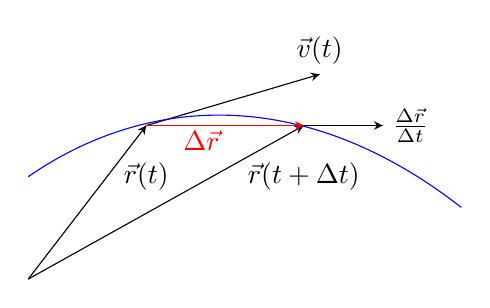
\begin{tikzpicture}[yscale=1.3]
    \draw [->] (0, 0) -- (3, 0) node [right] {$\frac{\Delta \vec{r}}{\Delta t}$};
    \draw [->] (0, 0) -- (2.2, 0.5) node [above] {$\vec{v}(t)$};
    \draw [->] (-1.5, -1.5) -- (0, 0) node at (0,-0.5) {$\vec{r}(t)$};
    \draw [->] (-1.5, -1.5) -- (2, 0) node at (2,-0.5) {$\vec{r}(t+\Delta t)$};
    \draw[color = Blue] (-1.5, -0.5) .. controls (0, 0.3) and (2, 0.4) .. (4, -0.8);
    \node[color = Red] at (0.7,-0.15) {$\Delta \vec{r}$};
	\draw[color = Red, ->] (0,0) -- (2,0);
  \end{tikzpicture}
\end{center}

\setlength{\jot}{8pt}% tweak jot length

Position: 
\[\vec{r}(t) = x(t)\hat{i} + y(t)\hat{j} + z(t)\hat{k}\]
At $\Delta t$ later
\[\vec{r}(t + \Delta t) = x(t + \Delta t)\hat{i} + y(t + \Delta t)\hat{j} + z(t + \Delta t)\hat{k}\]

\begin{definition}
Define the \textbf{Displacement Vector} $\Delta \vec{r} = \vec{r}(t + \Delta t) - \vec{r}(t)$

\end{definition}
\begin{definition}
Define the \textbf{velocity} of the particle at time $t$
\[\vec{v}(t) = \lim_{\Delta t \to 0} \frac{\Delta \vec{r}}{\Delta t} = \frac{\mathrm{d}\vec{r}}{\mathrm{d}t}\]
\end{definition}

Since $\hat{i},\hat{j},\hat{k}$ are constant in time
\[\begin{aligned}
	\vec{v}(t) = \frac{\mathrm{d}}{\mathrm{d}t}(\vec{r}(t)) &= \frac{\mathrm{d}}{\mathrm{d}t}(x \hat{i} + y\hat{j} + z\hat{k})\\
	&= \frac{\mathrm{d}x}{\mathrm{d}t}\hat{i} + \frac{\mathrm{d}y}{\mathrm{d}t}\hat{j} + \frac{\mathrm{d}z}{\mathrm{d}t}\hat{k}
\end{aligned}
\]
\textbf{Notation}

Writing $\dfrac{\mathrm{d}f}{\mathrm{d}t} \equiv \dot{f}$ (\emph{dot is shorthand for ``time derivative'' due to Newton})

We can write $\vec{v}(t)$ as \[\vec{v}(t) = \dot{x}\hat{i} + \dot{y}\hat{j} + \dot{z}\hat{k}\]

can also write \[\vec{v}(t) = v_x\hat{i} + v_y\hat{j} + v_z\hat{k}\]

\begin{definition}
\[v = |\vec{v}| = [v_x^2 + v_y^2 + v_z^2]^{1/2}\]
is the magnitude of the velocity or \textbf{speed} of the particle.

Thus, the \textbf{direction} of motion is 
\[\hat{v} = \vec{v}/v,~ |\hat{v}| = 1\]
$\hat{v}$ is also the unit tangent to the path of the object.
\end{definition}

\begin{definition}
Define the \textbf{acceleration}
\[\vec{a}(t) = \frac{d\vec{v}}{dt} = \frac{d^2\vec{r}}{dt^2} = \ddot{x}\hat{i} + \ddot{y}\hat{j} + \ddot{z}\hat{k}\]
\end{definition}

$\vec{a}(t)$ tells us how the velocity is changing at time $t$. 

Recall that we can write $\vec{v} = v(t)\hat{v}(t)$, then
\[\vec{a} = \frac{d}{dt}(v\hat{v}) = \underbrace{\frac{dv}{dt}\hat{v}}_{\substack{\text{Due to change}\\ \text{in speed}}} + \underbrace{v\frac{d\hat{v}}{dt}}_{\substack{\text{Due to change}\\ \text{in direction}}}\]

\begin{note}
This is the starting point for \textbf{intrinsic coordinates}.
\end{note}

We've started with $\vec{r}$ and we differentiated w.r.t $t$ to find $\vec{v}$ and $\vec{a}$. But, more usefully (as we often want to find $\vec{r}(t)$) we can start with $\vec{a}$ and integrate to find $\vec{v}$, then $\vec{r}$. 
\[\int_{t_0}^{t} \vec{a}dt' = \int_{t_0}^{t} \frac{d\vec{v}}{dt'}\,dt' = \vec{v}(t) - \vec{v}(t_0)
\]
\[\implies \vec{v}(t) = \vec{v}(t_0) + \int_{t_0}^t \vec{a}\,dt'\]

We can integrate this component-wise. For example 
\[v_x(t) = v_x(t_0) + \int_{t_0}^t a_x\,dt'\]
To determine $\vec{v}(t)$ uniquely, we need to know $\vec{v}(t_0)$ (constant vector). 

Similarly,
\[\vec{r}(t) = \vec{r}(t_0) + \int_{t_0}^t \vec{v}(t')\,dt'\]
Thus, starting with $\vec{a}(t)$, we need to know \emph{both} $\vec{r}(t_0)$ and $\vec{v}(t_0)$ to find $\vec{r}(t)$ uniquely! 

\begin{center}
\begin{tikzpicture}[node distance=2cm, auto]
  \node (P) {};
  \node (B) [right of=P] {$\vec{v}(t)$};
  \node (A) [below of=P] {$\vec{v}(t)$};
  \node (C) [below of=B] {$\vec{a}(t)$};
  \node (P1)[node distance=0.5cm, left of=P, above of=P] {$\vec{r}(t)$};
  %\draw[->] (P) to node {$\bar{f}$} (B);
  %\draw[->] (P) to node [swap] {$\bar{g}$} (A);
  \draw[->, bend right] (A) to node [swap] {$\dfrac{d}{dt}$} (C);
  \draw[<-, bend left] (B) to node {$\vec{v}(t_0) + \int_{t_0}^t \vec{a}\,dt'$} (C);
  \draw[->, bend right] (P1) to node [swap] {$\dfrac{d}{dt}$} (A);
  \draw[<-, bend left] (P1) to node {$\vec{r}(t_0) + \int_{t_0}^t\vec{v}\,dt'$} (B);
  %\draw[->, dashed] (P1) to node {$k$} (P);
\end{tikzpicture}
\end{center}

What allows us to connect the mathematics to the physical world is that these quantities are measurable. (\emph{e.g. ``It's cold out, it's only 5 degrees'' is meaningless. We need to specify units!})\\

\begin{definition}[SI Units]\begin{itemize}
\item \emph{Time:} Measured in seconds, s

\item \emph{Distance:} Measured in metres, m

\item \emph{Velocity:} ``Metres per second'', m/s or ms$^{-1}$
	
\item \emph{Acceleration}: ``Metres per second squared'', m/s$^2$ or ms$^{-2}$
\end{itemize}
\end{definition}\vsp

Can use units to ``maybe check'' that you've done a problem correctly.\\

\lecturemarker{3}{19 Jan}

\begin{example}[Acceleration due to Gravity]
	Near the surface of the earth, the acceleration due to gravity is \textbf{constant}
	\[g = 9.8ms^{-2}\]
	Suppose: an object is dropped \emph{from rest} at height $h$ above the ground. Find $\vec{r}(t)$:
	\vspace*{-5pt}
	\begin{center}
	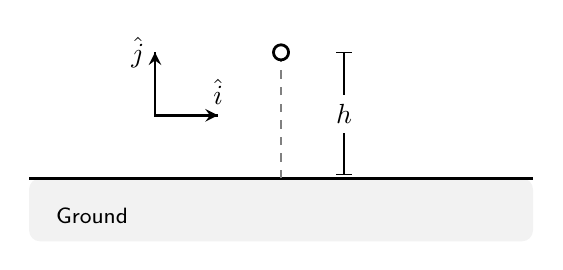
\begin{tikzpicture}[scale=.8,
    media/.style={font={\footnotesize\sffamily}},
    wave/.style={
        decorate,decoration={snake,post length=1.4mm,amplitude=2mm,
        segment length=2mm},thick},
    interface/.style={
        % The border decoration is a path replacing decorator. 
        % For the interface style we want to draw the original path.
        % The postaction option is therefore used to ensure that the
        % border decoration is drawn *after* the original path.
        postaction={draw,decorate,decoration={border,angle=-45,
                    amplitude=0.3cm,segment length=2mm}}},
    ]
    % Round rectangle
    \fill[gray!10,rounded corners] (-4,-1) rectangle (4,0);
    % Interface
    %\draw[black,line width=.5pt,interface](-4,0)--(4,0);
    \draw[-,line width=1pt] (-4,0) --(4,0);

    % Vertical dashed line
    \draw[dashed,gray](0,0)--(0,2);
    
        % Vertical dashed line
    \draw[|-|](1,0.05)--(1,2) node[midway,fill=white]{$h$};
    
        % Coordinates system
    \draw[<->,line width=1pt] (-1,1) node[above]{$\hat{i}$}-|(-2,2) node[left]{$\hat{j}$};

    % Media names
    \path[media] (-3,-.6) node {Ground};

    % $x$ axis
    \filldraw[fill=white,line width=1pt](0,2)circle(.12cm);

\end{tikzpicture}
	\end{center}

	Choose a coordinate system such that $\hat{j}$ points upwards. Then acceleration due to gravity is \[\vec{a} = -g\hat{j}\] We only have motion in the $\hat{j} \implies$ problem is 1D.
	
	We know initially ($t=0$) that $y(0) = h \implies v_y(0) = 0$. Integrate to find $v_y(t)$
    \[v_y(t) = \equalto{v_y(0)}{0} - \int_0^t g\, dt' = -gt\]

    Integrate again to find $y(t)$
    \[y(t) = \equalto{y(0)}{h} - \int_0^t gt\, dt' = h - \frac{1}{2}gt^2\]

\end{example}\vsp


\begin{example}[Projectiles]
Find $\alpha$ that maximises distance thrown ($d$).
\begin{center}
	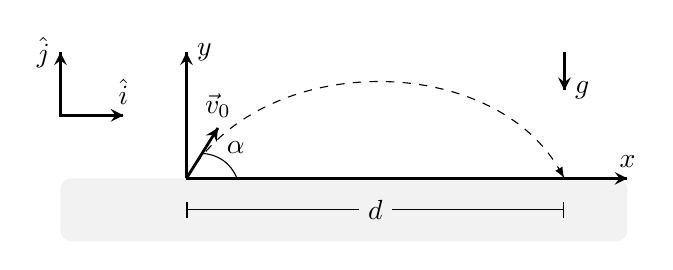
\begin{tikzpicture}[scale=.8,
    media/.style={font={\footnotesize\sffamily}},
    wave/.style={
        decorate,decoration={snake,post length=1.4mm,amplitude=2mm,
        segment length=2mm},thick},
    interface/.style={
        % The border decoration is a path replacing decorator. 
        % For the interface style we want to draw the original path.
        % The postaction option is therefore used to ensure that the
        % border decoration is drawn *after* the original path.
        postaction={draw,decorate,decoration={border,angle=-45,
                    amplitude=0.3cm,segment length=2mm}}},
    ]
    % Round rectangle
    \fill[gray!10,rounded corners] (-5,-1) rectangle (4,0);
    
    % Interface
    %\draw[blue,line width=.5pt,interface](-5,0)--(4,0);

    % Vertical dashed line
    %\draw[gray](-3,0)--(-3,2);
    
    % Coordinates system
    \draw[->,line width=1pt] (-3,0) --(4,0) node[above]{$x$};
    \draw[->,line width=1pt] (-3,0) --(-3,2) node[right]{$y$};
    
    % Coordinates system
    \draw[<->,line width=1pt] (-4,1) node[above]{$\hat{i}$}-|(-5,2) node[left]{$\hat{j}$};
    
    \draw[->,line width=1pt] (3,2)--(3,1.4) node[right]{$g$};

    \draw[->,line width=1pt] (-3,0)--(-2.5,0.8) node[above]{$\vec{v}_0$};


	 % Horizontal dashed line
    \draw[|-|](-3,-0.5)--(3,-0.5) node[midway, fill = gray!10]{$d$};


    % Media names
    %\path[media] (-3,-.6) node {Ground};
    
    
    \path (-3.2,0.3)++(11:1cm)node{$\alpha$};
    \draw[-](-2.2,0)arc(20:90:.6cm);

    
    % Interface pointer
    \draw[-latex,dashed](-3,0) to[out=60,in=120] (3,0);
    % To-paths are really useful for drawing curved lines. The above
    % to path is equal to:
    %
    % \draw[-latex,thick](3.2,0.5)node[right]{$\mathsf{S_{1,2}}$}
    %      ..controls +(180:.2cm) and +(up:0.25cm) .. (3,0);
    % Internally the to path is translated to a similar bezier curve,
    % but the to path syntax hides the complexity from the user. 

\end{tikzpicture}
	\end{center}
	
	In this coordinate system $\vec{a} = -g\hat{j}$. Choose that $t = 0$ when the object is released. Based on this \[\vec{r}(0) = \vec{0}\]

    and from the coordinate system
    \[\vec{v}(0) = v_0\cos\alpha\hat{i} + v_0\sin\alpha\hat{j} = \vec{v}_0 \implies v_0 = |\vec{v_0}|\]

    Integrate component-wise
    \[v_x(t) = v_x(0) + \int_0^t a_x(t')\,dt' = v_0\cos(\alpha)\]
    For $\hat{j}$ direction
    \[v_y(t) = v_y(0) + \int_0^t a_y(t')\,dt' = v_0\sin(\alpha) - gt\]

    \[\therefore \vec{v}(t) = v_0\cos(\alpha)\hat{i} + (v_0\sin(\alpha) - gt)\hat{j}\]

% todo finish this off
	Integrate our acceleration to find $\vec{v}(t)$
	\[\begin{aligned}\vec{v}(t) &= \vec{v}(0) + \int_0^t -g\hat{j}\,dt' = \vec{v}_0 -gt\hat{j} \\ 
	&= v_0\cos\alpha\hat{i} + (v_0\sin\alpha -gt)\hat{j}
\end{aligned}
\]
	Integrate our velocity to find the position
	\[\begin{aligned}
\vec{r}(t) &= \vec{r}(0) + 	\int_0^t \vec{v}(t)\,dt' = \vec{0} + \int_0^t\vec{v}_0 -gt'\hat{j}\,dt'\\
&= \vec{v}_0t - \textstyle{\frac{1}{2}}t^2g\hat{j} = v_0t\cos\alpha\hat{i} + [v_0t\sin\alpha - \textstyle{\frac{1}{2}}t^2g]\hat{j}
\end{aligned}
\]

Now, we want to find $d$, but first need to find the time $t_H$ that the object hits the ground.
% Maximise the \emph{range} using $\alpha$ as the control parameter. Finding the time $t_H$ when the object hits the ground.
$y(t_H) = 0$ where $y = \vec{r}\cdot\hat{j}$.
\[y = \vec{r}\cdot\hat{j}= v_0t_H\sin\alpha -\textstyle{\frac{1}{2}}t_H^2g = 0\]
Two values of $t_H$:
\[t_H = 0,~ t_H = \frac{2v_0\sin\alpha}{g}\]

To find $d = x(t_H)$:
\[d = x(t_H) = v_0\cos\alpha\left[\frac{2v_0\sin\alpha}{g}\right] = \frac{v_0^2}{g}\sin 2\alpha\]

For $0 \leq \alpha \leq \pi/2$, the max value of $d$ is achieved when $\alpha = \pi/4$.
\end{example}~\\

\begin{example}[Circular Motion]
\[\vec{r}(t) = R\sin(\Omega t)\hat{i} + R\cos(\Omega t)\hat{j}\quad (R,\Omega >0)\]

Distance from the origin 
\[r = |\vec{r}| = [R^2\sin^2\Omega t + R^2\cos^2\Omega t]^{1/2} = R\]

Path is a circle of radius $R$, centred at the origin. 

\begin{center}
  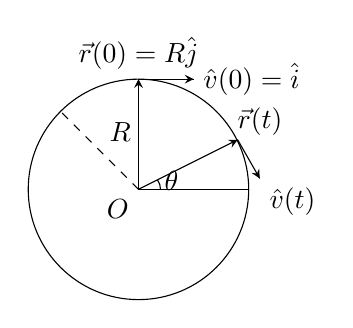
\begin{tikzpicture}[scale=.7]
    \draw circle [radius = 2];
    \node [anchor = north east] {$O$};
    \draw [->] (0, 0) -- (0, 2) node [above] {$\vec{r}(0) = R\hat{j}$};
    \draw (0, 0) -- (2, 0);
    \draw [dashed] (0, 0) -- (-1.4, 1.4) node [pos = 0.5, anchor = south west] {$R$};
    \draw [->] (0, 0) -- (1.8, 0.9) node [pos = 0.9, anchor = south west] {$\vec{r}(t)$};
    %\draw [->] (1.4, 1.4) -- (1.8, 1.8) node [anchor = south west] {$\hat{\mathbf{z}}$};
    \draw [->] (1.8, 0.9) -- (2.2, 0.2) node [anchor = north west] {$\hat{v}(t)$};
    \draw [->] (0, 2) -- (1, 2) node [anchor = west] {$\hat{v}(0) = \hat{i}$};
    \draw (0.4, 0) arc (0:35:0.3);
    \node at (0.6, 0.15) {$\theta$};
  \end{tikzpicture}
\end{center}

Differentiate $\vec{r}(t)$ to find 
\[\vec{v}(t) = R\Omega \cos \Omega t\hat{i} - R\Omega \sin \Omega t \hat{j}\]

Find the speed: $v = |\vec{v}| = R\Omega$, the speed is constant. 

\emph{Clockwise or anticlockwise?}

Direction of motion
\[\hat{v}= \vec{v}/v = \cos \Omega t\hat{i} - \sin\Omega t \hat{j}\]
At $t = 0$, $\hat{r}(0) = \hat{j}$ and $\hat{v}(0) = \hat{i}$, so it moves clockwise around the circle!\\

\emph{Interpretation of $\Omega$:} Introduce $\theta(t) = -\Omega t + \pi/2$ then $\frac{d\theta}{dt} = - \Omega$. ($\frac{\pi}{2}$ is initial angle and $-\Omega$ since we're moving clockwise at rate $\Omega$).

The parameter $\Omega$ is angular speed. Differentiate our $\vec{v}(t)$ we find
\[\begin{aligned}
\vec{a}(t) &= -R\Omega^2 \sin[\Omega t]\hat{i} - R\Omega^2\cos[\Omega t]\hat{j}\\
&= -\Omega^2 \vec{r}	
\end{aligned}
\]
Acceleration is pointing in towards the circle. i.e. in opposite direction to position vector and perpendicular to direction of motion. This is consistent with what we knew because the speed is constant.
\end{example}

\textbf{Last time:}  \lecturemarker{4}{5 Oct}
\[\vec{r}(t) = R\sin\Omega t \hat{i} + R\cos\Omega t \hat{j}\]
\begin{center}
  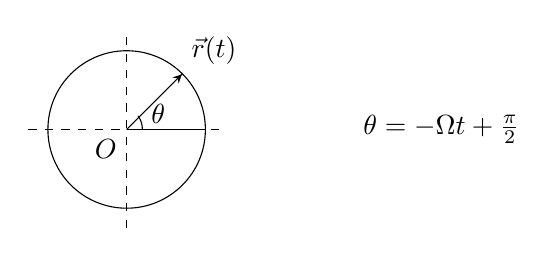
\begin{tikzpicture}
    \draw circle [radius = 1];
    \node [anchor = north east] {$O$};
    \draw [dashed, -] (0, -1.25) -- (0, 1.25);
    \draw [dashed, -] (-1.25,0) -- (1.25,0);
    \draw (0, 0) -- (1, 0);
    \draw [->] (0, 0) -- (0.7, 0.7) node [anchor = south west] {$\vec{r}(t)$};
    \draw (0.2, 0) arc (0:35:0.3);
    \node at (0.4, 0.2) {$\theta$};
    \node at (4,0) {$\theta = -\Omega t + \frac{\pi}{2}$};
  \end{tikzpicture}
\end{center}
\[\vec{r}(t) = R\cos[\theta(t)]\hat{i} +R\sin[\theta(t)]\hat{j}\]

Insert expression for $\theta$
\[\begin{aligned}
\vec{r}(t) &= R\cos[\pi/2 - \Omega t]\hat{i} + R\sin[\pi/2 - \Omega t]\hat{j} \\
&= R(\cancelto{0}{\cos\pi/2}\cos\Omega t + \cancelto{1}{\sin\pi/2}\sin\Omega t)\hat{i}\\
&+ R(\cancelto{1}{\sin\pi/2}\cos\Omega t - \cancelto{0}{\cos\pi/2}\sin\Omega t)\hat{j}\\
&= R\sin\Omega t \hat{i} + R\cos\Omega t \hat{j}
\end{aligned}
\]\vsp

\begin{example}[Wheel rolling without slipping ($\Omega, u$ constant)]

Describe the position of a point on the surface of the wheel

\[\vec{r}(t) = \equalto{\vec{r}_\Omega(t)}{\text{motion along a circle}} + \equalto{\vec{r}_c(t)}{\text{translation of the wheel}}\]
\begin{center}
  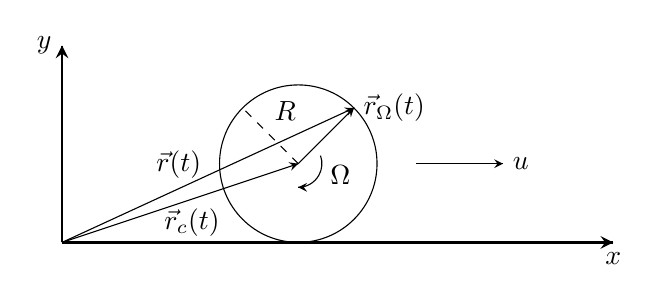
\begin{tikzpicture}
    \draw (0, 1) circle [radius=1];
    \draw [->] (0, 1) -- (0.707, 1.707) node [pos=1, anchor = west] {$\vec{r}_\Omega(t)$};
    \draw [->] (-3, 0) -- (0.707, 1.707) node [pos=0.4, above] {$\vec{r}(t)$};
    \draw [dashed] (0, 1) -- (-0.707, 1.707) node [pos=0.6, anchor = south west] {$R$};
    \draw [->] (1.5, 1) -- (2.6, 1) node [right] {$u$};
    \draw (0, 0.7) arc (270:380:0.3) node [anchor = north west] {$\Omega$};
    \draw [->] (-3,0) -- (0,1) node [pos = 0.55, below] {$\vec{r}_c(t)$};
    \draw [->] (0.01, 0.7) -- (0, 0.7);
    
    % Coordinates system
    \draw[->,line width=1pt] (-3,0) --(4,0) node[right, below]{$x$};
    \draw[->,line width=1pt] (-3,0) --(-3,2.5) node[left]{$y$};
    
  \end{tikzpicture}
\end{center}\vspace*{-5pt}
\[\begin{aligned}
\vec{r}_\Omega(t) &= R\cos\theta(t)\hat{i} + R\sin\theta(t)\hat{j}\\
\vec{r}_c(t) &= x_c(t)\hat{i} + R\hat{j}	
\end{aligned}
\]

Rolling at a constant angular speed: $\Omega$.\\
We are translating to the right with constant velocity: $u$.

Suppose initially $x_c(0) = 0,~ \theta(0) = \pi/2$. 

Then $x_c(y) = ut$ and $\theta = \pi/2 - \Omega t$. 

\[\begin{aligned}
\vec{r}_\Omega(t)f &= R\sin\Omega t \hat{i} + R\cos\Omega t \hat{j}\\
\vec{r}_c(t) &= ut\vec{i} + R\vec{j}\\
\vec{r}(t) &= [ut + R\sin(\Omega t)]\hat{i} + R[1 + \cos\Omega t]\hat{j}\\
\end{aligned}
\]

Here, $u$, and $\Omega$ are still independent of one another. We use ``rolling without slipping'' to connect them:\\

\textbf{Rolling without slipping:}
%todo fix theta to point down in these diagrams
\begin{center}
  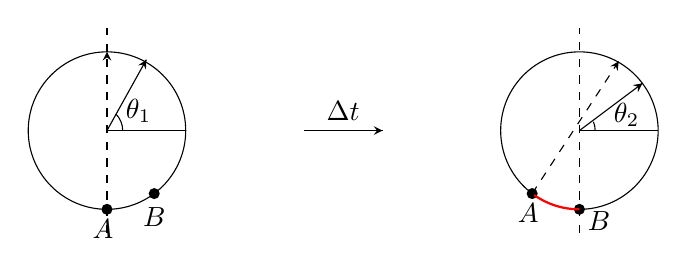
\begin{tikzpicture}
    \draw circle [radius = 1];
    \node at (-0.05,-1.25) {$A$};
    \fill (0,-1) circle (2pt);
    \node at (0.6,-1.1) {$B$};
    \fill (0.6,-0.8) circle (2pt);
    \draw [dashed, ->] (0, -1.3) -- (0, 1);
    \draw [dashed, -] (0,1) -- (0,1.3);
    \draw (0, 0) -- (1, 0);
    \draw [->] (0, 0) -- (0.5, 0.9);
    \draw (0.2, 0) arc (0:45:0.3);
    \node at (0.4, 0.25) {$\theta_1$};
    
    \draw [->] (2.5,0) -- (3.5,0) node [pos =0.5, above] {$\Delta t$};
    
    \draw (6,0) circle [radius = 1];
    \node at (5.35,-1.05) {$A$};
    \fill (5.4,-0.8) circle (2pt);
    \node at (6.25,-1.15) {$B$};
    \fill (6,-1) circle (2pt);
    \draw [dashed, -] (6, -1.3) -- (6, 1.3);
    \draw [dashed, ->] (5.4,-0.8) -- (6.5,0.88);
    \draw (6, 0) -- (7, 0);
    \draw [->] (6, 0) -- (6.8, 0.6);
    \draw (6.2, 0) arc (0:22:0.3);
    \node at (6.6, 0.2) {$\theta_2$};
    \draw [thick, red] (6,-1) arc (-90:-125:1); 
  \end{tikzpicture}
\end{center}


Rolling without slipping implies that the distance travelled equals the arc length between $A$ and $B$. 
\[\frac{|\Delta x_c|}{\Delta t} = R\frac{(\theta_2 - \theta_1)}{\Delta t}\]

Taking the limit as $\Delta t \to 0$
\[|\dot{x}_c| = R\dot{\theta}\]

By our convention, as $x$ increases, $\theta$ decreases, so
\[\dot{x}_c = -R\dot{\theta}\]
For our problem 
\[\dot{x}_c = u, \quad \dot{\theta} = -\Omega, \quad \boxed{u = R\Omega}\]

with this expression, we can eliminate $u$ and the position becomes
\[\vec{r}(t) = R[\Omega t + \sin(\Omega t)]\hat{i} + R[1 + \cos\Omega t]\hat{j}\]

Differentiate w.r.t $t$
\[\vec{v}(t) = R\Omega[1+ cos(\Omega t)]\hat{i} - R\Omega\sin(\Omega t)\hat{j}\]

Differentiating again
\[\begin{aligned}
\vec{a}(t) &= -R\Omega^2[\sin(\Omega t)\hat{i} + \cos(\Omega t)\hat{j}]\\
&= -\Omega^2\vec{r}_\Omega(t)
\end{aligned}
\]

\textbf{Sketch the path:}
\begin{center}
    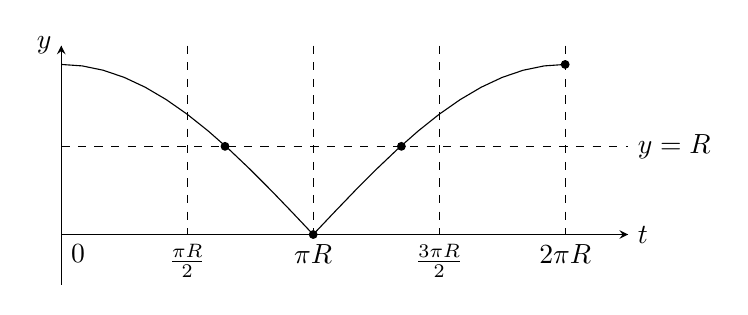
\begin{tikzpicture}[scale=.8]
      \draw [domain=0:4] plot ({2*\x}, {abs(2.7*(cos(45*\x)))});
      \draw [->] (0, 0) -- (9, 0) node [right] {$t$};
      \draw [->] (0, -0.8) -- (0, 3) node [left] {$y$};
      \draw [dashed] (0, 3) -- (0, 0) node [below right] {$0$};
      \draw [dashed] (8, 3) -- (8, 0) node [below] {$2\pi R$};
      \draw [dashed] (4, 3) -- (4, 0) node [below] {$\pi R$};
      \draw [dashed] (2, 3) -- (2, 0) node [below] {$\frac{\pi R}{2}$};
      \draw [dashed] (6, 3) -- (6, 0) node [below] {$\frac{3\pi R}{2}$};
      \draw [dashed] (0, 1.4) -- (9, 1.4) node [right] {$y = R$};  
      \fill (4,0) circle (2pt);    
      \fill (5.4,1.4) circle (2pt);  
      \fill (2.6,1.4) circle (2pt);   
      \fill (8,2.7) circle (2pt);       
    \end{tikzpicture}
  \end{center} 
At $x_c = \pi R \implies ut = \pi R$
\[y = \frac{\pi R}{u} = \frac{\pi}{\Omega}\]
\[\begin{aligned}
	\vec{v}(\pi/\Omega) &= R\Omega[1 + \cos[\Omega \pi/\Omega]]\hat{i} - R\Omega\sin[\Omega\pi/\Omega]\hat{j}\\
	&= \vec{0}
\end{aligned}
 \]
 
 Another way of expressing the condition is that the point on the wheel touching the ground has zero velocity \emph{relative} to the ground!

\end{example}


\subsektion{Vector Operations} 

Already \lecturemarker{5}{5 Oct} we have seen vector addition and subtraction are useful:

\textbf{Addition}: Rolling without slipping $\vec{r}(t) = \vec{r}_c(t) + \vec{r}_\Omega(t)$

\textbf{Subtraction}: Velocities relative to a moving observer $\vec{v}_{A,O} = \vec{v}_A - \vec{v}_O$

\begin{note}
    We can think of velocities relative to a moving observer as the concept of moving origins
\end{note}

\begin{example}
    Another way of think about ``rolling without slipping'' is the velocity of the point on the wheel touching the groud has zero velocity relative to the ground.

    \textbf{Recall}: $\vec{v}(t) = \left(u + R\Omega\cos(\Omega t)\right)\hat{i} - r\Omega\sin\Omega t\hat{j}$\\

    This point will touch the ground when $y(t) = 0$.
    \[
        y(t) = R(1 + \cos\Omega t) = 0 \implies \cos\Omega t = -1
    \]
    Can take $t = \frac{\pi}{\Omega}$
    \[
        \vec{v}(\frac{\pi}{\Omega}) = (u - R\Omega)\hat{i}
    \]
    since $\vec{v}(\frac{\pi}{\Omega})$ must be zero, $u = R\Omega$.
\end{example}

\subsubsektion{Vector Products}
 Vector products are also useful to describe mechanical phenomena: 

\textbf{(i) Scalar product (dot product)}

\begin{center}
    \begin{tikzpicture}[scale=.8]
      \draw [->] (0, 0) -- (4, 0) node [right] {$\vec{B}$};
      \draw [->] (0, 0) -- (2.5, 1.875) node [anchor = south west] {$\vec{A}$};
      \draw (0.7, 0) arc (0:36.87:0.7);
      \node at (0.9, 0.3) {$\theta$};
    \end{tikzpicture}
  \end{center}

\[\begin{aligned}
\vec{A} \cdot \vec{B} &= |\vec{A}||\vec{B}|\cos \theta\\
\vec{A} &= A_x\hat{i} + A_y\hat{j} + A_z\hat{k}\\
\vec{B} &= B_x\hat{i} + B_y\hat{j} + B_z\hat{k}\\
\vec{A}\cdot \vec{B} &= A_xB_x + A_yB_y + A_zB_z
\end{aligned}
\]

So we can write $|\vec{A}| = (\vec{A}\cdot\vec{A})^{1/2}$

The dot product can be used to pick out the component of a vector in a particular direction:
\[\hat{n},~|\hat{n}| = 1 \text{ (Direction)}\]

The component of $\vec{A}$ in $\hat{n}$-direction is 
\[A_n = \vec{A}\cdot\hat{n}\]

E.g. $\hat{n} = \hat{i}$, then 
\[\begin{aligned}
\vec{A}\cdot\hat{i} &= A_x(\hat{i}\cdot\hat{i}) + A_y\cancel{(\hat{j}\cdot{i})} + A_z\cancel{(\hat{i} \cdot\hat{k})}\\
&= A_x
\end{aligned}
\]~

\begin{example}
Acceleration tangent to the path of point on the surface of a wheel:

Recall:
\[
\begin{aligned}
\vec{v}(t) &= R\Omega[1 + \cos(\Omega t)]\hat{i} -R\Omega\sin(\Omega t)\hat{j}\\
\vec{a}(t) &= -R\Omega^2[\sin(\Omega t)\hat{i} + \cos(\Omega t)\hat{j}]
\end{aligned}
\]

Direction tangent to the path:
\[\frac{\vec{v}}{v} = \hat{v},~|\hat{v}| = 1\ \text{(by construction)}\]

Find: speed
\[\begin{aligned}
v^2 &= |\vec{v}|^2 = R^2\Omega^2(1 + 2\cos\Omega t + \cos^2\Omega t + \sin^2\Omega t)\\
v &= R\Omega\sqrt{2(1 + \cos\Omega t)}
\end{aligned}\]

The component of the acceleration tangent to the path 
\[\begin{aligned}
a_t &= \frac{\vec{a}\cdot\vec{v}}{v}\\
\vec{a} \cdot \vec{v} &= -R^2\Omega^3(\sin\Omega t + \sin\Omega t \cos\Omega t - \sin\Omega t \cos \Omega t]\\
&= -R^2\Omega^3\sin\Omega t\\
a_t &= -\frac{R\Omega^2\sin\Omega t}{\sqrt{2(1 + \cos\Omega t)}}
\end{aligned}
\]


\textbf{Recall} (intrinsic coordinates)

\begin{align*}
% todo fix
%\vec{a} &= \dfrac{d}{dt}(v(t)\hat{v}(t)) = \dfrac{dv}{dt}\hat{v} + v\dfrac{d\hat{v}}{dt}\\
%\vec{a}\dot\hat{v} &= \dfrac{dv}{dt}\ (\hat{v}\dot\dfrac{dv}{dt} = 0)
\end{align*}

\end{example}~

\textbf{(ii) Vector product (cross product)}

\[\begin{aligned}
\vec{A}\times \vec{B} &= \begin{vmatrix}
 \hat{i} & \hat{j} & \hat{k} \\
 A_x & A_y & A_z\\
 B_x & B_y & B_z	
 \end{vmatrix}\\
&= \hat{i}(A_yB_z - B_yA_z) + \hat{j}(A_zB_x - A_xB_z) + \hat{k}(A_xB_y - A_yB_x)
\end{aligned}
\]	

\begin{center}
    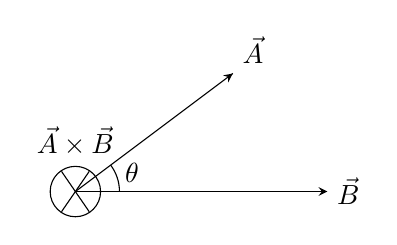
\begin{tikzpicture}[scale=.8]
      \draw [->] (0, 0) -- (4, 0) node [right] {$\vec{B}$};
      \draw [->] (0, 0) -- (2.5, 1.875) node [anchor = south west] {$\vec{A}$};
      \draw (0.7, 0) arc (0:36.87:0.7);
      \draw [-] (-0.22,-0.32) -- (0.22,0.32);
      \draw [-] (0.22, -0.32) -- (-0.22,0.32);
      \draw (0.4, 0) arc (0:360:0.4) node at (0,0.8) {$\vec{A} \times \vec{B}$};
      \node at (0.9, 0.3) {$\theta$};
    \end{tikzpicture}
  \end{center}
  \[|\vec{A} \times \vec{B} = |\vec{A}||\vec{B}|\sin\theta\]~
  
  The direction is given by the ``right hand rule'':
  \begin{center}
  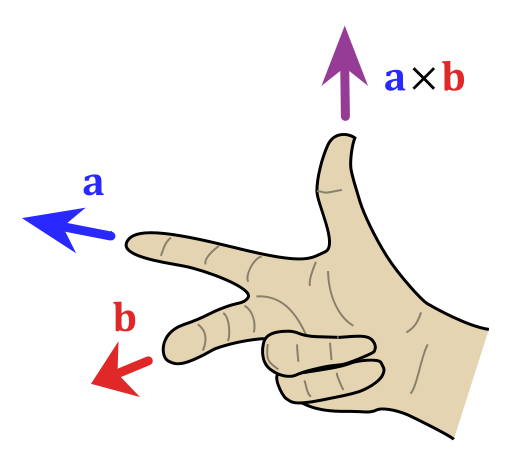
\includegraphics[width = 4cm]{right.png}	
  \end{center}

  
  \begin{example}
  Introduce $\vec{\omega} = -\Omega\hat{k},~(\Omega > 0)$
  
  \[
  \begin{aligned}
  \vec{r}_\Omega &= R\sin\Omega t\hat{i} + R\cos\Omega t\hat{j}\\
  \vec{\omega} \times \vec{r}_\Omega &= 
  \begin{vmatrix}
 \hat{i} & \hat{j} & \hat{k} \\
 0 & 0 & -\Omega \\
 R\sin\Omega t & R\cos\Omega t & 0 	
 \end{vmatrix}\\
 &= R\Omega \cos\Omega t\hat{i} -R\Omega \sin\Omega t\hat{j}\\
 &= \frac{d\vec{r}_\Omega}{dt} = \vec{v}_\Omega 
  \end{aligned}
  \]	
 

 $\Omega$: Angular speed
 
 $\vec{\omega}$: Angular velocity
 
 $-\hat{k}$ is the axis of rotation
  \end{example}
  
 What we have been doing really is thinking inside the box:
 
 
 \begin{center}
    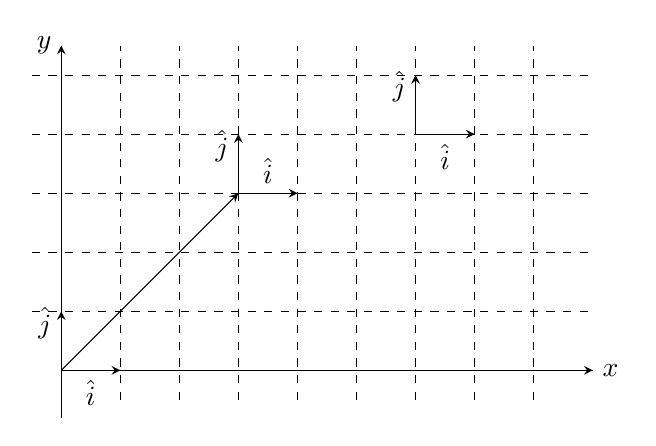
\begin{tikzpicture}[scale=.75]
      \draw [->] (0, 0) -- (9, 0) node [right] {$x$};
      \draw [->] (0, -0.8) -- (0, 5.5) node [left] {$y$};
      \foreach \x in {1,...,8}{
      \draw [dashed] (\x, -0.5) -- (\x, 5.5);}
      \foreach \y in {1,...,5}{
      \draw [dashed] (-0.5, \y) -- (9, \y);}
      \draw [->] (0,0) -- (3,3);
      \draw [->] (3,3) -- (3,4) node [pos = 0.8, left] {$\hat{j}$};
      \draw [->] (3,3) -- (4,3) node [pos = 0.5, above] {$\hat{i}$};
      \draw [->] (0,0) -- (0,1) node [pos = 0.8, left] {$\hat{j}$};
      \draw [->] (0,0) -- (1,0) node [pos = 0.5, below] {$\hat{i}$};
      \draw [->] (6,4) -- (6,5) node [pos = 0.8, left] {$\hat{j}$};
      \draw [->] (6,4) -- (7,4) node [pos = 0.5, below] {$\hat{i}$};
    \end{tikzpicture}
  \end{center} 
 
 
 $\hat{i}$: Points along lines of constant $y$ in the direction of increasing $x$
 
 $\hat{j}$: Points along lines of constant $x$ in the direction of increasing $y$
 

\subsektion{Plane Polar Coordinates}
We consider for 2D Motion. \lecturemarker{6}{5 Oct}  Certain systems simplify in these coordinates	



  \begin{center}
    \begin{tikzpicture}[scale=.75]
      \draw [->] (0, 0) -- (4, 0) node [right] {$x$};
      \draw [->] (0, 0) -- (0, 3) node [above] {$y$};
      \draw [dashed] (2.5,0) -- (2.5,2.5) node [pos = 0.5, right] {$y$};
      \node at (1.6,-0.3) {$x$};
      \draw (0, 0) -- (2.5, 2.5) node [circ]{} node [pos = 0.6, anchor = south east] {$r$};
      \draw (0.7, 0) arc (0:45:0.7);
      \node at (0.9, 0.3) {$\theta$};
    \end{tikzpicture}
  \end{center}
  
 We can relate $x$ and $y$ to $r$ and $\theta$:
 
\[\begin{aligned}
x &= r\cos\theta, \quad r = [x^2 + y^2]^{1/2}\\
y&= r\sin\theta, \quad \theta = \arctan(y/x)	
\end{aligned}
\]


 \begin{center}
 % todo should look more like a spider web with lines of constant theta drawn in
    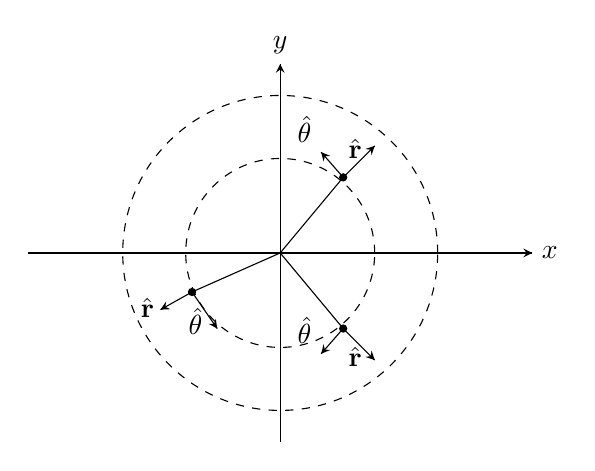
\begin{tikzpicture}[scale=.8]
      \draw [->] (-4, 0) -- (4, 0) node [right] {$x$};
      \draw [->] (0, -3) -- (0, 3) node [above] {$y$};
      \draw [dashed] circle [radius = 2.5];
      \draw [dashed] circle [radius = 1.5];
    
      \draw (0, 0) -- (1, 1.2) node [circ]{};
      \draw [->] (1, 1.2) -- (1.5, 1.7) node [pos = 0.9,left] {$\hat{\mathbf{r}}$};
      \draw [->] (1, 1.2) -- (0.65, 1.6) node [anchor = south east] {$\hat{\boldsymbol\theta}$};
      
      \draw (0, 0) -- (1, -1.2) node [circ]{};
      \draw [->] (1, -1.2) -- (1.5, -1.7) node [pos = 0.9,left] {$\hat{\mathbf{r}}$};
      \draw [->] (1, -1.2) -- (0.65, -1.6) node [anchor = south east] {$\hat{\boldsymbol\theta}$};
      
      \draw (0, 0) -- (-1.4, -0.62) node [circ]{};
      \draw [->] (-1.4, -0.62) -- (-1.9, -0.9) node [pos = 0.9,left] {$\hat{\mathbf{r}}$};
      \draw [->] (-1.4, -0.62) -- (-1, -1.2) node [pos = 0.8, left] {$\hat{\boldsymbol\theta}$};         
      
    \end{tikzpicture}
  \end{center}
$\hat{r}$: Unit vector in the direction of increasing $r$ along \textit{lines of constant $\theta$}.

$\hat{\theta}$: Points in the direction of increasing $\theta$ tangent to the \textit{circles of constant $r$}.\\

\begin{minipage}[c]{0.45\textwidth}
Consider: 

  \begin{center}
    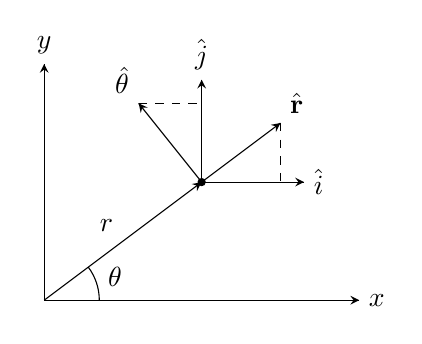
\begin{tikzpicture}
      \draw [->] (0, 0) -- (4, 0) node [right] {$x$};
      \draw [->] (0, 0) -- (0, 3) node [above] {$y$};
      \draw [->] (0, 0) -- (2, 1.5) node [circ]{} node [pos = 0.5, anchor = south east] {$r$};
      \draw [->] (2, 1.5) -- (3,2.25) node [anchor = south west] {$\hat{\mathbf{r}}$};
      \draw [->] (2,1.5) -- (2, 2.8) node [anchor = south] {$\hat{j}$}; 
      \draw [->] (2,1.5) -- (3.3, 1.5) node [anchor = west] {$\hat{i}$};
      \draw [->] (2, 1.5) -- (1.2, 2.5) node [anchor = south east] {$\hat{\boldsymbol\theta}$};
      \draw [dashed] (3,2.25) -- (3, 1.5);
      \draw [dashed] (1.2,2.5) -- (2,2.5);
      \draw (0.7, 0) arc (0:36.87:0.7);
      \node at (0.9, 0.3) {$\theta$};
    \end{tikzpicture}
  \end{center}
  \end{minipage}
 \begin{minipage}[c]{0.45\textwidth}
 ~\\
 \[\begin{aligned}
 |&\hat{r}| = |\hat{\theta}| = 1\\
	&\hat{r} = \cos\theta\hat{i} + \sin\theta\hat{j}\\
	&\hat{\theta} = -\sin\theta\hat{i} + \cos\theta\hat{j}
\end{aligned}
\]~

\begin{itemize}
\item They depend on $\theta$\\

\item $\hat{r} \cdot \hat{\theta} = 0$: \emph{orthonormal}	
\end{itemize}
\end{minipage}
\vspace*{1cm}

\begin{definition}[Kinematic Quantities in Polar Coordinates]~

\emph{Position}:
\[
\begin{aligned}
\vec{r} &= x\hat{i} + y\hat{j}\\
&= r\cos\theta\hat{i} + r\sin\theta\hat{j}\\
&= r[\underbrace{\cos\theta\hat{i} + \sin\theta\hat{j}}_{\hat{r}}]\\
\Aboxed{\vec{r} &= r(t)\hat{r}(t)}	
\end{aligned}
\]~

\emph{Velocity:}
\[
\begin{aligned}
  \vec{v} &= \frac{d}{dt}(\vec{r})\\
  &= \frac{d}{dt}(r\hat{r})\\
  &= \dot{r}\hat{r} + r\frac{d\hat{r}}{dt}\\[0.5cm]
  \frac{d}{dt}\hat{r} &= \frac{d}{dt}[\cos\theta(t)\hat{i} + \sin\theta(t)\hat{j}]\\
  &= -\sin\theta\dot{\theta}\hat{i} + \cos\theta\dot{\theta}\hat{j}\\
  &= \dot{\theta}[-\sin\theta\hat{i} + \cos\theta\hat{j}]\\
  &= \dot{\theta}\hat{\theta}\\
  \Aboxed{\vec{v} &= \dot{r}\hat{r} + r\dot{\theta}\hat{\theta}}
\end{aligned}
\]~

\emph{Acceleration}:
\[
\begin{aligned}
  \vec{a} &= \frac{d}{dt}(\vec{v})\\
  &= \frac{d}{dt}[\dot{r}\hat{r} + r\dot{\theta}\hat{\theta}]\\
  &= \ddot{r}\hat{r} + \dot{r}\frac{d\hat{r}}{dt} + \dot{r}\dot{\theta}\hat{\theta} + r\ddot{\theta}\hat{\theta} + r\dot{\theta}\frac{d\hat{\theta}}{dt}\\[0.5cm]
    \frac{d\hat{\theta}}{dt} &= \frac{d}{dt}[-\sin\theta\hat{i} + \cos\theta\hat{j}]\\
  &= -\cos\theta\dot{\theta}\hat{i} - \sin\theta\dot{\theta}\hat{j}\\
  &= -\dot{\theta}\hat{r}
\end{aligned}
\]
Thus
\[
\begin{aligned}
  \vec{a} &= (\ddot{r} - r\dot{\theta}^2)\hat{r} + (\dot{r}\dot{\theta} + \dot{r}\dot{\theta} + r\ddot{\theta})\hat{\theta} \\
 \Aboxed{\vec{a} &= (\ddot{r} - r\dot{\theta}^2)\hat{r} + (2\dot{r}\dot{\theta} + r\ddot{\theta})\hat{\theta}}
\end{aligned}
\]
\end{definition}\vsp


\begin{examples}
\begin{enumerate}
  \item Uniform Circular Motion:
  
  \[\vec{r}(t) = R\sin\Omega t\hat{i} + R\cos\Omega t \hat{j}\]
  The corresponding expression in polars:
  \[r = R \implies \dot{r} = 0,\quad \theta(t) = \frac{\pi}{2} - \Omega t \implies \dot{\theta} = -\Omega\]
  \[
\begin{aligned}
  \Aboxed{\vec{r} &= R\hat{r}}\\
  \vec{v} &= \equalto{\dot{r}}{0}\hat{r} + r\dot{\theta}\hat{\theta}\\
  \Aboxed{\vec{v} &= -R\Omega\hat{\theta}}\\
  \vec{a} &: \quad \ddot{r} = \ddot{\theta} = 0\\
  \Aboxed{\vec{a} &= -R\Omega^2\hat{r}}
\end{aligned}
\]~\\

\item (Bead on a bicycle spoke) Bead moves outwards with constant speed $u$ as the wheel turns with constant angular speed $\Omega$:
\begin{center}
  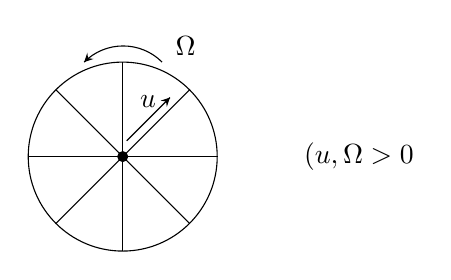
\begin{tikzpicture}
    \draw circle [radius = 1.2];
	\fill (0,0) circle (2 pt);
    \draw (0, -1.2) -- (0, 1.2);
    \draw (-1.2,0) -- (1.2,0);
    \draw (-0.85,-0.85) -- (0.85,0.85);
    \draw (-0.85,0.85) -- (0.85,-0.85);
    \draw [->] (0.05, 0.2) -- (0.6, 0.75) node [pos = 0.9, left] {$u$};
    \node at (3,0) {$(u,\Omega >0$};
    \draw [->] (0.5, 1.2) arc (45:135:0.7) node at (0.8,1.4) {$\Omega$};
  \end{tikzpicture}
\end{center}

%todo fix this - wanted to add since u... etc comments.
If at $t=0$:
\[r(0) = 0 \,\text{ \& }\, \theta(0) = 0\]
Since $u$ is outward velocity
\[\dot{r} = u\]
Since $\Omega$ is the angular speed and the wheel is rotating anti-clockwise
\[\dot{\theta} = \Omega\]
\[\implies r(t) = ut \,\text{ \& }\, \theta(t) = \Omega t	\]
\[\ddot{r} = 0, \ddot{\theta} = 0\]

\[
\begin{aligned}
  \vec{r} &= ut\hat{r}\\
  \vec{v} &= u\hat{r} + u\Omega t\hat{\theta}\\
  \vec{a} &= -u\Omega^2t\hat{r} + 2u\Omega\hat{\theta}
\end{aligned}
\]
\end{enumerate}
\end{examples}


Polar coordinates really come in handy when the forces have certain symmetries, e.g. Central forces: $\vec{F} = F(r)\hat{r}$.



\subsektion{Intrinsic Coordinates}

Coordinates \lecturemarker{7}{5 Oct}
 that are intrinsic to the path of our particle. Use ful when we know the path. Restrict our discussion to cases where the object move in one direction.
 
\begin{center}
  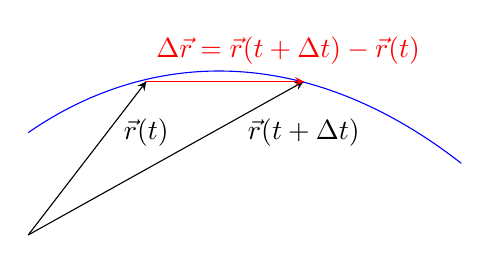
\begin{tikzpicture}[yscale=1.3]
    \draw [->] (-1.5, -1.5) -- (0, 0) node at (0,-0.5) {$\vec{r}(t)$};
    \draw [->] (-1.5, -1.5) -- (2, 0) node at (2,-0.5) {$\vec{r}(t+\Delta t)$};
    \draw[color = Blue] (-1.5, -0.5) .. controls (0, 0.3) and (2, 0.4) .. (4, -0.8);
    \node[color = Red] at (1.8,0.3) {$\Delta \vec{r} = \vec{r}(t + \Delta t) - \vec{r}(t)$};
	\draw[color = Red, ->] (0,0) -- (2,0);
  \end{tikzpicture}
\end{center}

Distance travelled between $t$ and $t + \Delta t$
:
\[\begin{aligned}\Delta s &= |\Delta \vec{r}|\\
& = \left|[x(t + \Delta t) - x(t)]\hat{i} + [y(t + \Delta t) - y(t)]\hat{j} + [z(t + \Delta t) - z(t)]\hat{k}\right|	
\end{aligned}
\]

For $\Delta t << 1$: 
\[x(t + \Delta t) = x(t) + \Delta t \frac{dx}{dt} + \cal{O}(\Delta t^2)\]
(Taylor series expansion of $x(t + \Delta t)$)

Doing the same for our other components and substituting:
\begin{align*}
\Delta s &= \left|\frac{dx}{dt}\hat{i} + \frac{dy}{dt}\hat{j} + \frac{dz}{dt}\hat{k}\right|\Delta t + \cal{O}(\Delta t^2)\\
&= \Delta t \equalto{|\vec{v}|}{\text{the speed, }v} + \cal{O}(\Delta t^2)
\end{align*}

Thus,
\[\frac{\Delta s}{\Delta t} = v + \cal{O}(\Delta t)\]

Taking $\lim \Delta t \to 0$
\[\begin{aligned}\Aboxed{\frac{ds}{dt} &= v = \dot{s}}\\ 
\implies s(t) &= \int_0^t v(t')\,dt'	
\end{aligned}
\]

Assuming $s = 0$ when $t = 0$. Both $s$ and $t$ are different parameterisations of the path. Instead of writing $\vec{r}(t)$, we can write $\vec{r}(s)$. \\

\begin{definition} $s$ is what we call the \emph{arc length}. 

\emph{Velocity}:
\[\vec{v} = \frac{d\vec{r}}{dt} = \frac{d\vec{r}}{ds}\frac{ds}{dt}\]
But $\displaystyle{\frac{ds}{dt} = v}$. Since this is the magnitude of $\hat{v}$, so it must be the case that \[\displaystyle{\frac{d\vec{r}}{ds} = \hat{v}}\] the unit tangent at evert point $s$. Thus, in intrinsic coordinates
\[\boxed{\vec{v}(s) = \dot{s}\hat{v}}\]

\emph{Acceleration}: \[\begin{aligned}
	\vec{a} &= \frac{d\vec{v}}{dt}\\ &= \frac{d}{dt}\left(\dot{s}~ \hat{v}\right)\\
	&= \ddot{s}\hat{v} + \dot{s}\dfrac{d\hat{v}}{dt}\\
% todo fix
%\intertext{But}
\dfrac{d\hat{v}}{dt} &= \dfrac{d}{dt}\left(\dfrac{d\hat{r}}{ds}\right)\\
&= \dfrac{d^2\hat{r}}{ds^2}\dfrac{ds}{dt} = \dfrac{d^2\hat{r}}{ds^2}\dot{s}\\
%\intertext{So, acceleration becomes}
	\vec{a} &= \ddot{s}\hat{v} + \dot{s}\frac{d^2\vec{r}}{ds^2}\frac{ds}{dt}\end{aligned}
\]

Writing $\displaystyle{\frac{d^2\vec{r}}{ds^2} = \kappa \hat{n}}$, where $\displaystyle{\kappa =\left|\frac{d^2\vec{r}}{ds^2}\right| }$, $\hat{n} = \displaystyle{\frac{1}{\kappa}\frac{d^2\vec{r}}{ds^2}}$, we have: 
\[\boxed{\vec{a}(s) = \ddot{s}\hat{v} + \kappa \dot{s}^2\hat{n}}\]

It turns out that $\kappa$ is the \emph{curvature} of the path. What about $\hat{n}$?

Recall: $|\hat{v}| = 1 $. So 
% todo \implies \hat{v} \dot \hat{v} = 0
\[\begin{aligned}\frac{d}{ds}(\hat{v}\cdot\hat{v} = 1)\\
 \implies 2\hat{v}\cdot\frac{d\hat{v}}{ds} = 0\\
% todo since \dfrac{d\hat{v}}{dt} = \frac{d^2\vec{r}}{ds^2} = \kappa \hat{n}
 \implies 2\kappa(\hat{v}\cdot\hat{n}) = 0	
\end{aligned}
\]

So, if $\kappa \neq 0$, then $\hat{v}\cdot \hat{n} = 0$. Thus $\hat{n}$ is the \emph{unit normal} to the path.
\end{definition}~

% todo missing from notes!
This is related to the local radius of curvature... TODO!\\

Tangential component of the acceleration $a_t = \vec{a}\cdot\hat{v} = \ddot{s}$

Normal component of the acceleration $a_n = \vec{a}\cdot\hat{n} = \kappa \dot{s}^2$, where $\kappa \approx 1/R$

\begin{center}
  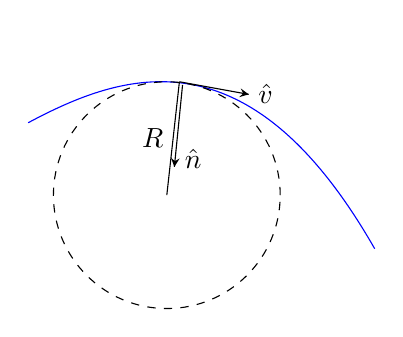
\begin{tikzpicture}[scale=.8]
    %\draw [->] (0, 0) -- (3, 0) node [right] {$\frac{\Delta \vec{r}}{\Delta t}$};
    %\draw [->] (0, 0) -- (2.2, 0.5) node [above] {$\vec{v}(t)$};
    %\draw [->] (-1.5, -1.5) -- (0, 0) node at (0,-0.5) {$\vec{r}(t)$};
    %\draw [->] (-1.5, -1.5) -- (2, 0) node at (2,-0.5) {$\vec{r}(t+\Delta t)$};
    \draw[color = blue] (-1.5, -0.5) .. controls (0, 0.3) and (2, 1) .. (4, -2.5);
    \draw [dashed] (0.7,-1.65) circle [radius = 1.8];
    \draw (0.7,-1.65) -- (0.9,0.15) node [pos = 0.5, left] {$R$};
    \draw [->] (0.95,0.1) -- (0.82,-1.2) node [pos = 0.9, right] {$\hat{n}$};
    \draw [->] (0.9,0.15) -- (2,-0.05) node [right] {$\hat{v}$};
    %\node[color = red] at (0.7,-0.15) {$\Delta \vec{r}$};
	%\draw[color = red, ->] (0,0) -- (2,0);
  \end{tikzpicture}
\end{center}


Key things to note:

\begin{enumerate}
    \item $\hat{v}, \hat{n}, \kappa$ depend only on the path (Knowing $\vec{r}(s)$, we can find these quantities)
    \item $\dot{s}$ and $\ddot{s}$ depend on how the particle is moving along the path
\end{enumerate}

\pagebreak


\begin{example}[Circular Motion]~

\emph{Cartesian:}
\[\begin{aligned}
\vec{r}(t) &= R\sin(\omega t)\hat{i} + R\cos(\omega t)\hat{j}\\
\vec{v}(t) &= \dots\\
\vec{a}(t) &= \dots
\end{aligned}
\]~\\


\emph{Polars:} 
$r = R$ and $\theta = \frac{\pi}{2} \omega t \implies \dot{r} = \ddot{r} = 0$ and $ \dot{\theta} = -\omega,~\ddot{\theta} = 0$. So 

\[\begin{aligned}
	\vec{r} &= R\hat{r}\\
 \vec{v} &= \dot{r}\hat{r} + r\dot{\theta}\hat{\theta} = -R\omega\hat{\theta}\\
\vec{a} &= (\ddot{r} - r\dot{\theta}^2)\hat{r} + (2\dot{r}\dot{\theta} + r\ddot{\theta})\hat{\theta} = -R\omega^2\hat{r}
\end{aligned}
\]~\\


\emph{Intrinsic:} ($s(0) = 0$) 

The speed is given by $v = R\omega = \dot{s} \implies \ddot{s} = 0$. Integrate to find $s$
\[s = R\omega t \implies t= \frac{s}{R\omega}\]

Substitute this into our expression for $\vec{r}(t)$
\[\vec{r}(s) = R\sin(s/R)\hat{i} + R\cos(s/R)\hat{j}\]

Tangent: 
\[\hat{v} = \dfrac{d\vec{r}}{ds} = \cos(s/R)\hat{i} - \sin(s/R)\hat{j}\]

Curvature and Normal:
\[\dfrac{d^2\vec{r}}{ds^2} = -\dfrac{1}{R}[\sin(s/R)\hat{i} + \cos(s/R)\hat{j}\]
\[ \kappa = \left|\dfrac{d^2\vec{r}}{ds^2} \right| = \dfrac{1}{R},~ \hat{n} = -\sin(s/R)\hat{i} - \cos(s/R)\hat{j}\]

Thus
\[\begin{aligned}
\vec{v}(s) &= R\omega \hat{v}\\
\vec{a}(s) &= \ddot{s}\hat{v} + \kappa \dot{s}^2\hat{n}\\
& = \frac{1}{R}(R\omega)^2\hat{n}\\ &= R\omega^2\hat{n}
\end{aligned}
\]
\end{example}

\pagebreak


\begin{example}[Helical Path]\lecturemarker{8}{5 Oct}
	\[\vec{r}(s) = b\cos(ks)\hat{i} + b\sin(ks)\hat{j} + s\sqrt{1-b^2k^2}\hat{k}\]
	
	Tangent:
	\[\hat{v} = \frac{d\vec{r}}{ds} = -bk\sin(ks)\hat{i} + bk\cos(ks)\hat{j} + \sqrt{1-b^2k^2}\hat{k}\]~
	
	Curvature and Normal:
	\[\frac{d^2\vec{r}}{ds^2} = -bk^2\cos(ks)\hat{i} -bk^2 \sin(ks)\hat{j}\]
	\[\kappa =\left|\frac{d^2\vec{r}}{ds^2}\right| = bk^2,~ \hat{n} =  -\cos(ks)\hat{i} -\sin(ks)\hat{j}\]
	
Take $s = ct$ ($c >0$) $ \implies \dot{s} =c,~ \ddot{s} = 0$. Thus
\[\vec{v} = c\hat{v},~\vec{a} = c^2bk^2\hat{n}\]	
\end{example}~

Take the case where our path lies in the $xy-$plane and we know $y(x)$
\begin{center}
\begin{tikzpicture}
\draw [->] (0,0) -- (6,0) node[pos = 1, below] {$x$}; 
\draw [->] (0,0) -- (0,4) node[pos = 0.9, left] {$y$};	
\draw[color = Blue] (0, 0.2) .. controls (1, 2) and (3, 2.2) .. (5.5, 3.8);
\fill (2,2) circle (2 pt);
\fill (3,2.5) circle (2 pt);
\draw [dashed] (2,2) -- (3,2) node [pos = 0.5,below] {$dx$};
\draw [dashed] (3,2) -- (3,2.5) node [pos = 0.5, right] {$dy$};
\draw [thick] (2,2) -- (3,2.5) node [pos = 0.5, above] {$ds$};
\end{tikzpicture}
\end{center}

Then $ds^2 = dx^2 + dy^2$. Since $dy = \dfrac{dy}{dx}dx$ 
\[\begin{aligned}
ds^2 &= \left(1 + \left(\frac{dy}{dx}\right)^2\right)dx^2\\
\implies \frac{ds}{dx} &= \sqrt{1 + y'^2}\quad y' = \frac{dy}{dx}\\
s(x) &= \int_{x_0}^x (1 + y'^2)^{1/2}dx
\end{aligned}\]

Highlights that $s$ just depends on the path. 


Position: \[\vec{r}(x) = x\hat{i} + y(x)\hat{j}\]

Tangent to the path
\[\hat{v} = \frac{d\vec{r}}{ds} = \frac{d\vec{r}}{dx}\frac{dx}{ds} = \frac{d\vec{r}}{dx}\left(\frac{ds}{dx}\right)^{-1}\]
\[\begin{aligned}
\frac{d\vec{r}}{dx} &= \hat{i} + y'\hat{j}\\
\left(\frac{ds}{dx}\right)^{-1} &= [1 + y'^2]^{-1/2}\\
\implies \Aboxed{\hat{v} &= [1+y'^2]^{-1/2}[\hat{i} + y'\hat{j}]}
\end{aligned}\]

Curvature and Normal:
\[\begin{aligned}
\frac{d^2\vec{r}}{ds^2} &= \frac{d}{dx}\left(\frac{d\vec{r}}{ds}\right)\left(\frac{ds}{dx}\right)^{-1}\\
&= \left(\frac{d}{dx}\left(\frac{d\vec{r}}{ds}\right)\frac{dx}{ds}\right)\\[0.5cm]
\frac{d}{dx}\left[\frac{d\vec{r}}{ds}\right] &= \frac{d\hat{v}}{dx}\\
 &= -\frac{1}{2}[1+y'^2]^{-3/2} \times (2y'y'')\times [\hat{i} + y'\hat{j}]\\
 &+ [1 + y'^2]^{-1/2}y''\hat{j}\\
 &= [1 + y'^2]^{-3/2}y'' \times (-y'\hat{i} + (1+y'^2 - y'^2)\hat{j})\\
 &= \frac{y''}{[1+y'^2]^{3/2}}(-y'\hat{i} + \hat{j})\\[0.5cm]
 \implies \frac{d^2\vec{r}}{ds^2} &= \frac{y''}{[1+y'^2]^{3/2}}\left(-\frac{y'}{[1+y'^2]^{1/2}}\hat{i} + \frac{1}{[1+y'^2]^{1/2}}\hat{j}\right)\\
 \Aboxed{\kappa &= \left|\frac{d^2\vec{r}}{ds^2}\right| = \frac{|y''|}{[1+y^2]^{3/2}}}\\
  \Aboxed{\hat{n} &= \frac{1}{\kappa} \frac{d^2\vec{r}}{ds^2} = \frac{y''}{|y''|}\frac{1}{[1+y'^2]^{1/2}}(-y'\hat{i} + \hat{j})}
\end{aligned}
\]~


\begin{center}
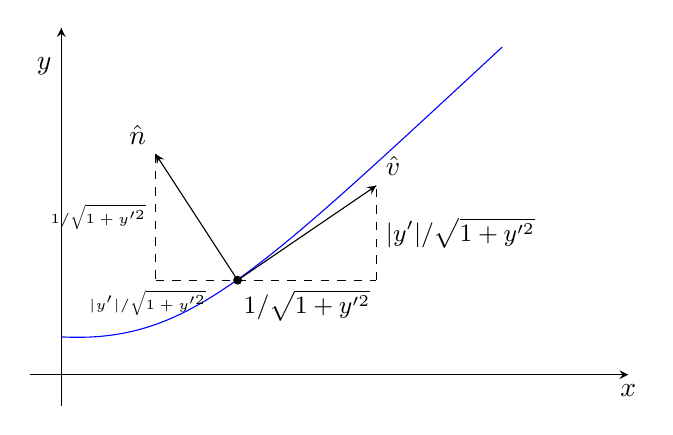
\begin{tikzpicture}[scale=.8]
\draw [->] (-0.5,0) -- (9,0) node[pos = 1, below] {$x$}; 
\draw [->] (0,-0.5) -- (0,5.5) node[pos = 0.9, left] {$y$};	
\draw[color = Blue] (0, 0.6) .. controls (2, 0.5) and (3, 1.5) .. (7, 5.2);
\fill (2.8,1.5) circle (2 pt);
\draw [dashed] (2.8,1.5) -- (5,1.5) node [pos = 0.5,below] {\small $1/\sqrt{1+y'^2}$};
\draw [dashed] (5,1.5) -- (5,3) node [pos = 0.5, right] {\small $|y'|/\sqrt{1+y'^2}$};

\draw [->] (2.8, 1.5) -- (5,3) node [anchor = south west] {$\hat{v}$};
\draw [->] (2.8, 1.5) -- (1.5, 3.5) node [anchor = south east] {$\hat{n}$};
      
\draw [dashed] (1.5,3.5) -- (1.5, 1.5) node [pos = 0.5, left] {\tiny $1/\sqrt{1+y'^2}$};
\draw [dashed] (1.5,1.5) -- (2.8,1.5) node [pos = -0.1, below] {\tiny $|y'|/\sqrt{1+y'^2}$};

\end{tikzpicture}
\end{center}
\vspace*{10pt}


\begin{example}
$y = x^2,~y' = 2x,~ y'' = 2$

\[\begin{aligned}
\frac{ds}{dx} &= [1 + y'^2]^{1/2}\\	
&= [1 + 4x^2]^{1/2}\\[0.5cm]
\hat{v} &= \frac{d\vec{r}}{dx}\left(\frac{ds}{dx}\right)^{-1}\\
&= (\hat{i} + 2x\hat{j})(1 + 4x^2)^{-1/2}\\[0.5cm]
\hat{n} &= (1 + 4x^2)^{-1/2}(-2x\hat{i} + \hat{j})\\
\kappa &= \frac{2}{[1+4x^2]^{3/2}}
\end{aligned}
\]	

Now all we need is $\dot{s}$ and $\ddot{s}$. If $\dot{s} =c,~\ddot{s} = 0$, then
\[\vec{v} = c\hat{v},~ \vec{a} = c^2\kappa\hat{n}.\]
\end{example}
%!TEX root = linear-algebra.tex

\sektion{Kinetics and Newtons Laws}
\subsektion{Newton's Laws}\vsp


\lecturemarker{9}{22 Oct}
\begin{definition}
\begin{itemize}

\item \emph{Mass, $m$} - ``Quantity of Matter'', measured in kg (scalar)

\item \emph{Momentum, $\vec{p} = m\vec{v}$} - ``Quantity of Motion'' (vector)

\item \emph{Inertia} - ``Vis Insita'' (innate force of matter). The resistance of an object to change its state of motion.

\item \emph{Force} - An action that changes an objects state of motion
\end{itemize}
\end{definition}~

\begin{theorem}[Newton's First Law]
Every body has inertia! 	
\end{theorem}

\begin{center}
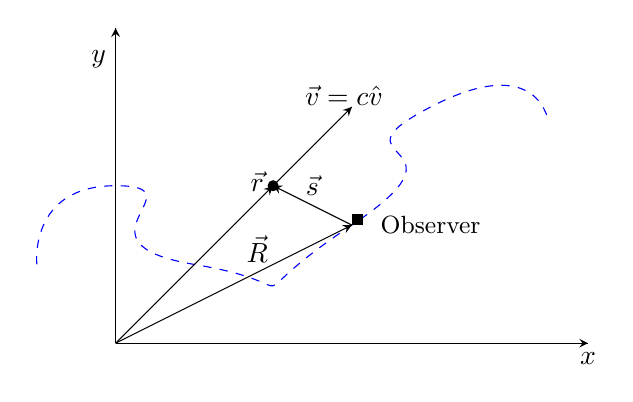
\begin{tikzpicture}
\draw [->] (0,0) -- (6,0) node[pos = 1, below] {$x$}; 
\draw [->] (0,0) -- (0,4) node[pos = 0.9, left] {$y$};	
\draw [dashed, color = Blue, yshift = -1cm] plot [smooth, tension=2] coordinates {(-1,2) (0,3) (1,2) (3,2.5) (4,4) (5.5,3.8)};
\fill (2,2) circle (2 pt);
\fill (3,1.5) rectangle ++(4pt,4pt); 
\node at (4,1.5) {\small Observer};
\draw [->] (0,0) -- (3,1.5) node[pos = 0.6,above] {$\vec{R}$};
\draw [->] (0,0) -- (2,2) node[pos = 0.9, above] {$\vec{r}$};
\draw [->] (2,2) -- (3,3) node [pos = 0.9, above] {$\vec{v} = c\hat{v}$};
\draw [->] (3,1.5) -- (2,2) node[pos = 0.5,above] {$\vec{s}$};
\end{tikzpicture}
\end{center}
\[
\begin{aligned}
  \vec{r} &= \vec{R} + \vec{s},~\vec{s} = \vec{r} - \vec{R}\\
  \frac{d\vec{s}}{dt} &= \frac{d\vec{r}}{dt} - \frac{d\vec{R}}{dt}\\
  \frac{d^2\vec{s}}{dt^2} &= \cancel{\frac{d^2\vec{r}}{dt^2}} - \frac{d^2\vec{R}}{dt^2}
\end{aligned}
\]

If $\dfrac{d^2\vec{R}}{dt^2} \neq 0$, then the object will not be maintaining its state of motion. 

Inertial frame $\dfrac{d^2\vec{R}}{dt^2} = 0$.\pagebreak




\begin{theorem}[Newton's Second Law]
The net force on an object is equal to the rate of change of momentum:

\[ \vec{F} = \frac{d\vec{p}}{dt} = \frac{d(m\vec{v})}{dt}\]
\end{theorem}

Alternatively 
\[\vec{p}(t) - \vec{p}(0) = \int_0^t \vec{F}(t')\,dt'\]

If the mass is constant we get the familiar $\vec{F} = m\vec{a}$.\\



\begin{theorem}[Newton's Third Law]
If $\vec{F}_{AB}$ is the force on object $A$ due to object $B$, then $\vec{F}_{BA} = -\vec{F}_{AB}$.
\end{theorem}

  \begin{center}
    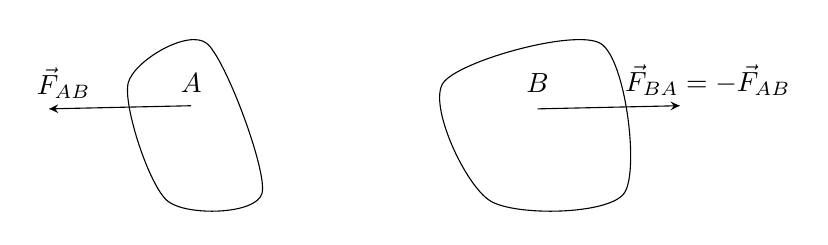
\begin{tikzpicture}
      \draw plot [smooth cycle] coordinates{(2,0.5) (4,1) (4.3,-0.9) (2.6,-1)};
      \draw plot [smooth cycle] coordinates{(-2,0.5) (-1,1) (-0.3,-0.9) (-1.5,-1)};
      \draw [<-] (-3, 0.17) -- (-1.2, 0.21) node [pos = 0.1, above] {$\vec{F}_{AB}$};
      \node at (-1.2,0.5) {$A$};
      \node at (3.2,0.5) {$B$};
      \draw [->] (3.2, 0.17) -- (5, 0.21) node [pos = 1.2, above] {$\vec{F}_{BA} = -\vec{F}_{AB}$};
    \end{tikzpicture}
  \end{center}
  

\begin{theorem}[Conservation of Linear Momentum]
	Momentum is conserved in a closed system with no external forces.
\end{theorem}

\begin{proof}
Total momentum:
\[\begin{aligned}
\vec{p}_T &= \vec{p}_A + \vec{p}_B\\
\frac{d\vec{p}_T}{dt} &= \frac{d\vec{p}_A}{dt} + \frac{d\vec{p}_B}{dt}	
\end{aligned}
\]

Assume $\vec{F}_{AB}$ is the only force on $A \implies$ only force on $B$ is $-\vec{F}_{AB}$. 

\[\frac{d\vec{p}_T}{dt} = \vec{F}_{AB} - \vec{F}_{AB} = \vec{0}\]
\end{proof}


%!TEX root = M1A1.tex
\sektion{Forces}

Kinds \lecturemarker{10}{22 Oct}
 of forces:
\begin{enumerate}
\item Constraint Forces
\item Forces can also depend on our kinematic quantities
\item Forces can depend on velocity. ``Drag Force''
\item Forces can also depend on position	
\end{enumerate}

\subsektion{Gravity}

  \begin{center}
    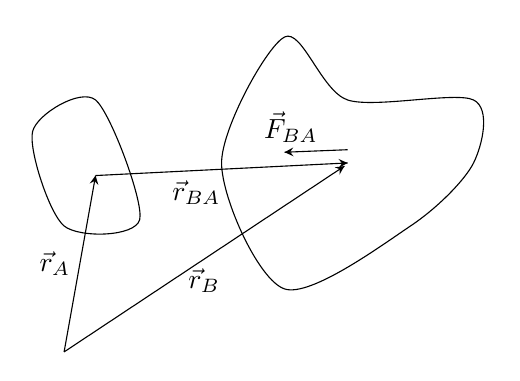
\begin{tikzpicture}[scale = 0.8]
      \draw plot [smooth cycle] coordinates{(1, 0) (2, -2)  (4, -1)  (5, 0)  (5, 1)  (3, 1)  (2, 2)};
      \draw plot [smooth cycle] coordinates{(-2,0.5) (-1,1) (-0.3,-0.9) (-1.5,-1)};
      \draw [->] (-1.5, -3) -- (-1, -0.2) node [pos =0.5, left] {$\vec{r}_A$};
      \draw [->] (-1.5, -3) -- (2.95, -0.05) node [pos = 0.5, below] {$\vec{r}_B$};
      \draw [<-] (2, 0.17) -- (3, 0.21) node [pos = 0.1, above] {$\vec{F}_{BA}$};
      \draw [->] (-1, -0.2) -- (3, 0) node [pos = 0.4, below] {$\vec{r}_{BA}$};
    \end{tikzpicture}
  \end{center}

The force on $m_b$ due to $m_A$ is 
\[
\begin{aligned}
\vec{F}_{BA} &= -\frac{Gm_Am_b}{r^2_{BA}}\hat{r}_{BA}\\
r_{BA} &= |\vec{r}_{BA}|\\
\hat{r}_{BA} &= \frac{\vec{r}_{BA}}{r_{BA}}
\end{aligned}
\]

\begin{itemize}
\item $G$ is the gravitational constant 
\[G = 6.67 \times 10^{-11} m^3/kgs^2\]	
\item $\vec{F}_{BA}$ is attractive
\item The magnitude of force decays like $1/r^2_{BA}$ 
\item This is a central force - $\vec{F} = F(r)\hat{r}$
\end{itemize}

Recall that we said that the acceleration due to gravity is constant! $\implies |\vec{F}_g| = mg$.

We can say this because the force due to gravity acts from the centre of the earth, and the change in height of our object is small compared to the radius of the earth.

And the change in height of our object be small compared to the radius of the earth.\\

\emph{How small does the height need to be? How do we show this?} 

\begin{center}
  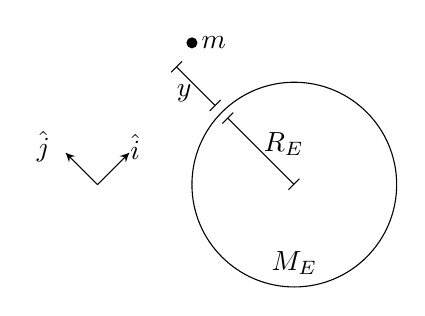
\begin{tikzpicture}
    \draw circle [radius = 1.3];
	\node at (0,-1) {$M_E$};
    \draw [|-|] (-0.85,0.85) -- (0,0) node [pos = 0.4, right] {$R_E$};
	\draw [|-|] (-1,1) -- (-1.5,1.5) node [pos = 0.8, below] {$y$};
	\fill (-1.3,1.8) circle (2pt) node [right] {$m$};	
	\draw [->] (-2.5,0) -- (-2.1,0.4) node [pos = 1.2] {$\hat{i}$};	
	\draw [->] (-2.5,0) -- (-2.9,0.4) node [pos = 1.2, left] {$\hat{j}$};
  \end{tikzpicture}
\end{center}

Using Newton's Formula:
\[\vec{F}_g = -\frac{GmM_E}{(y+R_E)^2}\hat{j}\]

If $y =0$
\[\vec{F}_g = -\frac{GmM_E}{R_E^2}\hat{j}\]

If we write 
\[\vec{F}_g = -mg\hat{j}\]

The $g = \frac{GM_E}{R^2_E} = 9.8m/s^2$. Rewrite $\vec{F}_g$:
\[\vec{F}_g = -mg[1 + y/R_E]^{-2}\hat{j}\]

We know that $y/R_E << 1$. This allows us to use a taylor series about $y/R_E = 0$ to approximate $[1 + y/R_E]^{-2}$. Taylor series about $x = 0$:
\[f(x) = f(0) + f'(0)x + \textstyle{\frac{1}{2}f''(0)x^2 + \dots }\]

In our case $x = y/R_E$
\[
\begin{aligned}
f(x) &= [1+x]^{-2} \quad f(0) = 1\\
f'(x) &= -2[1+x]^{-3} \quad f'(0) = -2\\
f''(x) &= 6[1+x]^{-4} \quad f''(0) = 6\\
\implies \vec{F}_g &= mg(1-2\frac{y}{R_E})\hat{j} + \mathcal{O}(y^2/R^2_E)
\end{aligned}
\]
So taking $\vec{F}_g = -mg\hat{j}$ is equivalent to using the first term in the taylor series.\\

\begin{example}[For Felix] $y = 39 \times 10^3m \quad R_E = 6371 \times 10^3m$.

Suppose we use the constant force 
\[\vec{F}_g = -mg\hat{j}\]
Using our linear approximation 
\[\vec{F}_g = -0.9878mg\hat{j}\]
Actual $\vec{F}_g = -0.9879mg\hat{j}$. 
\end{example}

We are interested in using the force to predict where the object will be.

Using Newton's II Law and the Newtonian Gravity
\[m\frac{d^2y}{dt^2} = -\frac{GmM_E}{(R_E + y)^2}\]

Constant approximation:
\[\begin{aligned}m\frac{d^2y}{dt^2} &= -mg\\
\implies y(t) &= y_0 + v_0t + \frac{1}{2}gt^2	
\end{aligned}
\]

Linear approximation:
\[m\frac{d^2y}{dt^2} = -mg(1-2y/R_E)\]


\subsektion{Contraint Forces}

Force \lecturemarker{11}{22 Oct} that arise only to satisfy or enforce a particular constraint on the motion of a body. These forces arise when we have 
\begin{enumerate}
\item Surfaces
\item Wires
\item Strings and Bars	
\end{enumerate}~

\begin{example}
	\begin{center}
	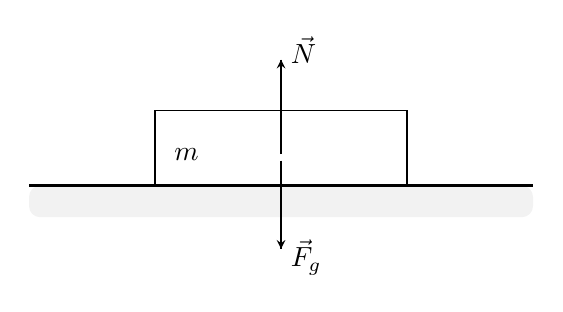
\begin{tikzpicture}[scale=.8,
    media/.style={font={\footnotesize\sffamily}},
    wave/.style={
        decorate,decoration={snake,post length=1.4mm,amplitude=2mm,
        segment length=2mm},thick},
    interface/.style={
        postaction={draw,decorate,decoration={border,angle=-45,
                    amplitude=0.3cm,segment length=2mm}}},
    ]
    % Round rectangle
    \fill[gray!10,rounded corners] (-4,-0.5) rectangle (4,0);
	
	\draw (-2,0) rectangle (2,1.2);
	\node at (-1.5,0.5) {$m$};

    %\draw[black,line width=.5pt,interface](-4,0)--(4,0);
    \draw[-,line width=1pt] (-4,0) --(4,0);

    % Vertical dashed line
    \draw[->](0,0.5)--(0,2) node [pos = 1.1, right] {$\vec{N}$};
    \draw[->](0,0.4)--(0,-1) node [pos = 1.1, right] {$\vec{F}_g$};
    

\end{tikzpicture}
	\end{center}

$\vec{N}$ exists to keep the object from going through the surface.
\end{example}

\begin{definition}
$\vec{N}$ is called the \emph{Normal} or \emph{Reaction} Force.	
\end{definition}


\begin{center}
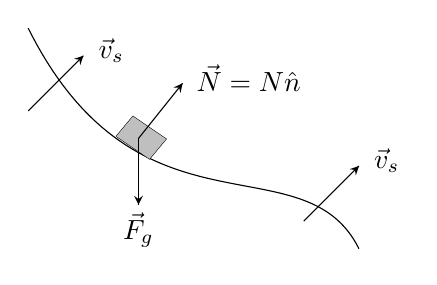
\begin{tikzpicture}[scale = 0.7]
\draw (-2,4) .. controls (0,0) and (3,2) .. (4,0);
\draw (-0.4,2.04) -- (-0.1,2.4) -- (0.5,1.99) -- (0.2,1.63) -- (-0.4,2.04);
\fill[gray!50]  (-0.4,2.04) -- (-0.1,2.4) -- (0.5,1.99) -- (0.2,1.63) -- (-0.4,2.04);
\draw [->] (0,2) -- (0,0.8) node[pos = 1.8, above] {$\vec{F}_g$};
\draw [->] (0,2) -- (0.8,3) node [pos = 1.1, right] {$\vec{N} = N\hat{n}$};
\draw [->] (-2,2.5) -- (-1,3.5) node [pos = 1.1, right] {$\vec{v}_s$};
\draw [->] (3,0.5) -- (4,1.5) node [pos = 1.1, right] {$\vec{v}_s$};
\end{tikzpicture}
\end{center}



$\vec{N}$ acts in a direction normal (or perpendicular) to the surface. 

If our surface has a velocity $\vec{v}_s$, then 
\[\vec{v} \cdot\hat{n} = \vec{v}_s \cdot\hat{n}\]

 $\vec{N}$ only exists when the object is in contact with the surface $\implies N \geq 0$. For wires, everything is more or less the same, except that $N \iR$. 

We can use different coordinate systems to find the normal force:\\

\begin{minipage}[c]{8cm}
\begin{enumerate}

  \item \leavevmode\vadjust{\vspace{-\baselineskip}}\newline
  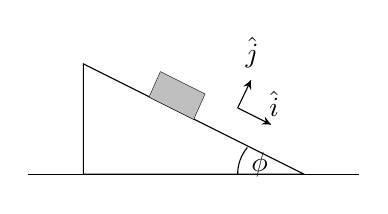
\begin{tikzpicture}[scale = 0.7]
  	\draw (0,0) -- (6,0);
  	\draw (1,0) -- (5,0) -- (1,2) -- (1,0);
  	\draw (3.8, 0) arc (180:140:0.75);
  	\node at (4.2,0.18) {$\phi$};
    \draw (2.2,1.4) -- (3,1) -- (3.2,1.45) -- (2.4, 1.85) -- (2.2,1.4);
    \fill[gray!50] (2.2,1.4) -- (3,1) -- (3.2,1.45) -- (2.4, 1.85) -- (2.2,1.4);
    \draw [->] (3.8,1.2) -- (4.04,1.7) node [pos = 1.1, above] {$\hat{j}$};
    \draw [->] (3.8,1.2) -- (4.4,0.9) node [pos = 1.1, above] {$\hat{i}$};
  \end{tikzpicture}~\\[0.5cm]
  
 

  \item \leavevmode\vadjust{\vspace{-\baselineskip}}\newline
  \hspace*{1cm}
  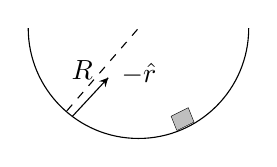
\begin{tikzpicture}[scale = 0.7]
    \draw [dashed] (0.7,-1.5) -- (2,0) node [pos = 0.5, left] {$R$};
    \draw [->] (0.8, -1.6) -- (1.45, -0.9) node [pos = 1.1, right] {$-\hat{r}$};
    \draw (2.7,-1.85) -- (3,-1.7) -- (2.9,-1.45) -- (2.6, -1.6) -- (2.7,-1.85);
    \fill[gray!50] (2.7,-1.85) -- (3,-1.7) -- (2.9,-1.45) -- (2.6, -1.6) -- (2.7,-1.85);
    \draw (0,0) arc (180:360:2);
  \end{tikzpicture}~\\[0.5cm]

 
\item \leavevmode\vadjust{\vspace{-\baselineskip}}\newline
\hspace*{1cm}
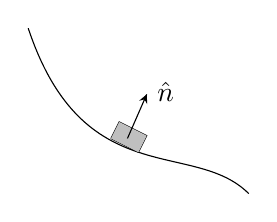
\begin{tikzpicture}[scale = 0.7]
\draw (-1,3) .. controls (0,0) and (2,1) .. (3,0);
\draw (0.5,1) -- (0.65,1.3) -- (1.15,1.05) -- (1,0.75) -- (0.5,1);
\fill[gray!50] (0.5,1) -- (0.65,1.3) -- (1.15,1.05) -- (1,0.75) -- (0.5,1);
\draw [->] (0.8,1) -- (1.15,1.8) node [pos = 1.05, right] {$\hat{n}$};
\end{tikzpicture}

\end{enumerate}~

\end{minipage}
\begin{minipage}[c]{6cm}
  $\vec{N} = N\hat{j}$. 
  
  Constraint: $\dot{y} = 0$ ($\vec{v}_s = 0$)\\[2cm]
  
  $\vec{N} = -N\hat{r}$.
  
  Constraint: $\dot{r} = 0$.\\[1.5cm]
  
  (In 2D) $\hat{n} = \frac{1}{\kappa}\frac{d^2\vec{r}}{ds^2}$.\\[0.1cm]
  
  $\vec{N} = N\hat{n}$.
  
  Constraint: $\vec{v} \cdot \hat{n} = 0$.\\[1cm] 
 \end{minipage}
 
 \begin{example}\vspace*{-20pt}
 \begin{center}
 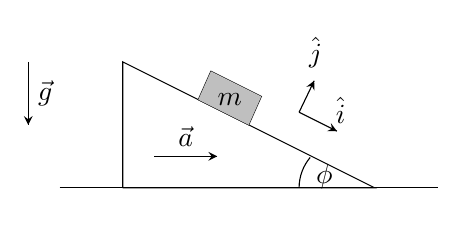
\begin{tikzpicture}[scale = 0.8]
  	\draw (0,0) -- (6,0);
  	\draw (1,0) -- (5,0) -- (1,2) -- (1,0);
  	\draw (3.8, 0) arc (180:140:0.75);
  	\node at (4.2,0.18) {$\phi$};
    \draw (2.2,1.4) -- (3,1) -- (3.2,1.45) -- (2.4, 1.85) -- (2.2,1.4);
    \fill[gray!50] (2.2,1.4) -- (3,1) -- (3.2,1.45) -- (2.4, 1.85) -- (2.2,1.4);
    \draw [->] (3.8,1.2) -- (4.04,1.7) node [pos = 1.1, above] {$\hat{j}$};
    \draw [->] (3.8,1.2) -- (4.4,0.9) node [pos = 1.1, above] {$\hat{i}$};
    \node at (2.7,1.4) {$m$};
    \draw [->] (-0.5,2) -- (-0.5,1) node [pos = 0.5, right] {$\vec{g}$};
    \draw [->] (1.5,0.5) -- (2.5,0.5) node [pos = 0.5, above] {$\vec{a}$};
  \end{tikzpicture}
  \end{center}
  
 $\vec{a}$ is constant. Find: $\vec{a}_m$ (acceleration of $m$) and $\vec{N}$. 
 
 Setting up the equations is important! [See: Kleppner \& Kolenkow \S 2.4]


Force diagram: \vspace*{-10pt} 
\begin{center}
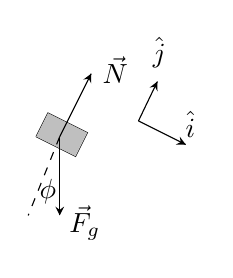
\begin{tikzpicture}
\draw (0.5,1) -- (0.65,1.3) -- (1.15,1.05) -- (1,0.75) -- (0.5,1);
\fill[gray!50] (0.5,1) -- (0.65,1.3) -- (1.15,1.05) -- (1,0.75) -- (0.5,1);
\draw [->] (0.8,1) -- (0.8,0) node [pos = 1.1, right] {$\vec{F}_g$};
\draw [dashed] (0.8,1) -- (0.4,0);
\draw [->] (0.8,1) -- (1.2,1.8) node [pos = 1.05, right] {$\vec{N}$};
\draw [->] (1.8,1.2) -- (2.04,1.7) node [pos = 1.1, above] {$\hat{j}$};
\draw [->] (1.8,1.2) -- (2.4,0.9) node [pos = 1.1, above] {$\hat{i}$};
\node at (0.65,0.3) {$\phi$};
\end{tikzpicture}	
\end{center}

Constraints: 
 \[
\begin{aligned}
  \vec{v}_s\cdot \hat{n} &= \vec{v}\cdot\hat{n}\\
  \hat{n} = \hat{j} &\implies \dot{y}_s = \dot{y}_m\\
  &\implies \ddot{y}_s = \ddot{y}_m
\end{aligned}
\]

Express forces in the coordinate system: 
\[
\begin{aligned}
  \vec{N} &= N\hat{j}\\
  \vec{F}_g &= mg[\sin\phi \hat{i} - \cos\phi \hat{j}]\\
  \vec{a} &= a[\cos\phi\hat{i} + \sin\phi\hat{j}]
\end{aligned}
\]

Use Newton's Laws:
\[
\begin{aligned}
  m\vec{a}_m &= \vec{F}_g + \vec{N}\\
  ma_{mx} &= mg\sin\phi\\
  ma_{my} &= -mg\cos\phi + N
\end{aligned}
\]

From our constraint: 
\[\implies a\sin\phi = a_{my}\]

Substitute this into Newton's Second Law: 
\[
\begin{aligned}
  ma\sin\phi &= -mg\cos\phi + N\\
  \implies \Aboxed{N &= m[a\sin\phi + g\cos\phi]}
\end{aligned}
\]

Our final unknown is given directly by Newton's II: $a_{mx} = g\sin\phi$, so
\[\boxed{\vec{a}_m = g\sin\phi \hat{i} + a\sin\phi\hat{j}}\]
The mass will not move relative to the surface if: 
\[
\begin{aligned}
  \vec{a}_m &= \vec{a}\\
  \implies \vec{a}_m\cdot\hat{i} &= \vec{a}\cdot\hat{i}\\
  \implies g\sin\phi &= a\cos\phi\\
  a/g &= \tan\phi 
\end{aligned}
\]

If $g\sin\phi < a\cos\phi$ the block slides off the top. 

If $g\sin\phi > a\cos\phi$ the block slides down the ramp. 

\end{example}\vsp



\begin{example}[\href{https://www.youtube.com/watch?v=qybUFnY7Y8w}{OK Go Video}]
\lecturemarker{12}{22 Oct}
\begin{center}
\begin{tikzpicture}
	\draw [dashed] (0,0) arc (270:140:2);
	\draw (-0.5,-0.5) rectangle (0.5,0.5);
	\draw [dashed] (0,0) -- (0,4); 
	\draw (-1.6,3.5) -- (-1.1,3.8) -- (-0.9,3.55) -- (-1.4,3.25) -- (-1.6,3.5);
	\draw (-1.2,3.38) -- (-0.1,1.82) -- (0,1.9)-- (-1.05,3.45);
	\draw [->] (-3,3) -- (-3,2) node [pos = 1.6, above] {$\vec{g}$};
	\draw[<->,line width=1pt] (2,2) node[above]{$\hat{j}$}-|(3,3) node[left]{$\hat{i}$};
	\node at (-0.15,2.5) {$\theta$};
	\draw (0,2.8) arc (90:130:0.8); 
	\draw [->] (-0.8, 3.45) -- (-0.4, 2.9) node at (0.5,3.2) {$\vec{T} = -T\hat{r}$};
	\node at (-1, 2.4) {$R$};
\end{tikzpicture}	
\end{center}


We know that the distance between $m$ and a point in space remains constant. We can use polar coordinates to solve the problem because we have information about  $r, (\dot{r}, \ddot{r})$ or $\theta, \dot{\theta}, \ddot{\theta}$. In this case we know $r = R$ (constant) $\implies \dot{r} = \ddot{r} =0$. This will be enforced by $\vec{T}$, the \emph{tension}. In our coordinate system:
\[
  \vec{T} = -T\hat{r}
\]

Find: $T$ and also $\vec{v}$ at $\theta = \pi$. 

Force diagram: 
\begin{center}
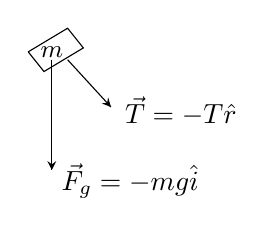
\begin{tikzpicture}
	\draw (-1.6,3.5) -- (-1.1,3.8) -- (-0.9,3.55) -- (-1.4,3.25) -- (-1.6,3.5);
\node at (-1.3,3.5) {\small $m$};
\draw [->] (-1.3,3.4) -- (-1.3,2) node [pos = 1.1, right] {$\vec{F}_g = -mg\hat{i}$};
\draw [->] (-1.1,3.4) -- (-0.55,2.8) node [pos = 1.1, right] {$\vec{T} = -T\hat{r}$};
\end{tikzpicture}	
\end{center}


\[
\begin{aligned}
  (\hat{r} &= \cos\theta \hat{i} + \sin\theta\hat{j})\times \cos\theta\\
  + (\hat{\theta} &= -\sin\theta\hat{i} + \cos\hat{j})\times -\sin\theta
\end{aligned}
\]
\[
  \cos\theta\hat{r} - \sin\theta\hat{\theta} = \hat{i}
\]
\[
  \implies \vec{F}_g = -mg[\cos\theta\hat{r} - \sin\theta\hat{\theta}]
\]

Newton's Laws:
\[
\begin{aligned}
  m\vec{a} &= \vec{T} + \vec{F}_g\\
  \implies m[(\ddot{r} - r\dot{\theta}^2)\hat{r} + (r\ddot{\theta} + 2\dot{r}\dot{\theta})\hat{\theta}] &= -T\hat{r} -mg\cos\theta\hat{r} + mg\sin\theta\hat{\theta}
\end{aligned}
\]

$\hat{r}$ component: 
\[
  m(\ddot{r} - r\dot{\theta}^2) = -T-mg\cos\theta \tag{i}
\]

$\hat{\theta}$ component:
\[
  m(r\ddot{r} + 2\dot{r}\dot{\theta}) = mg\sin\theta \tag{ii}
\]

Use the constraint in Newton's II Law: $r = R$, $\dot{r} = \ddot{r} = 0$. 
\[
\begin{aligned}
  \mathrm{(i)} &\implies -mR\dot{\theta}^2 = -T-mg\cos\theta \\
  \mathrm{(ii)} &\implies mR\ddot{\theta} = mg\sin\theta
\end{aligned}
\]

Take (ii) $\times \dot{\theta} \implies mR\ddot{\theta}\dot{\theta} = mg\sin\theta\dot{\theta}$. 

Notice 
\[
\begin{aligned}
  \ddot{\theta}\dot{\theta} &= \frac{1}{2}\frac{d}{dt}(\dot{\theta}^2)\\
  \sin\theta\dot{\theta} &= \frac{d}{dt}(-\cos\theta)
\end{aligned}
\]
\[
\begin{aligned}
    \frac{d}{dt}(\frac{1}{2}\dot{\theta}^2 + \frac{g}{R}\cos\theta) &= 0\\
  \implies \frac{1}{2}\dot{\theta}^2 + \frac{g}{R}\cos\theta &= K \text{ (constant!)}
\end{aligned}
\]

Take $t = 0, \theta = \theta_0, \dot{\theta} = 0$

\[
\begin{aligned}
\implies K &= \frac{g}{R}\cos\theta_0\\
\implies \dot{\theta}^2 &= \frac{2g}{R}[\cos\theta_0 - \cos\theta]  
\end{aligned}
\]

In polar coordinates: 
\[
\begin{aligned}
  \vec{v} &= \dot{r}\hat{r} + r\dot{\theta}\hat{\theta}\\
  \vec{v} &= R\dot{\theta}\hat{\theta}
\end{aligned}
\]~

At the bottom when the hammer hits the TV, $\theta = \pi$

\[
\begin{aligned}
  \implies \dot{\theta}^2 &= \frac{2g}{R}[\cos\theta_0 + 1]\\
  \vec{v} &= R\sqrt{\frac{2g}{R}[\cos\theta_0 + 1]}\hat{\theta}
\end{aligned}
\]

At $\theta = \pi, \hat{\theta} = -\hat{j}$. We can find the tension from (i): 
\[-mR\dot{\theta}^2 = -T - mg\cos\theta\]

Using our expression for $\dot{\theta}^2$
\[
\begin{aligned}
  +mR[\frac{2g}{R}[\cos\theta_0 -\cos\theta]] &= +T + mg\cos\theta\\
  \implies \Aboxed{T = 2mg\cos\theta_0 &-3mg\cos\theta} 
\end{aligned}
\]
\end{example}\vsp


\begin{example}[Strings]  \lecturemarker{13}{22 Oct}\vspace*{-20 pt}
\begin{center}
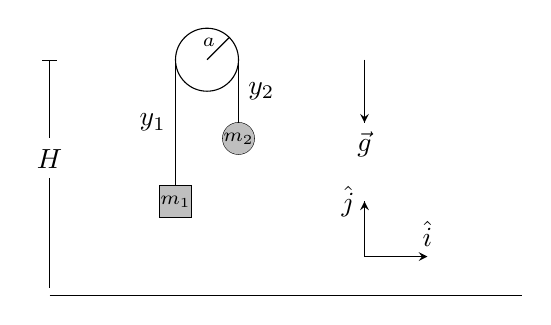
\begin{tikzpicture}
\draw (1.4,1) rectangle (1.8,1.4);
\draw (2,3) circle (0.4cm);
\draw (0,0) -- (6,0);
\draw (2.4,2) circle (0.2cm);
\fill[gray!50] (2.4,2) circle (0.2cm);
\fill[gray!50] (1.4,1) rectangle (1.8,1.4);
\node at (1.6, 1.2) {\scriptsize $m_1$};
\node at (2.4,2) {\scriptsize $m_2$};
\draw (1.6,1.4) -- (1.6,3) node [pos = 0.5, left] {$y_1$};
\draw (2.4,2.2) -- (2.4,3) node [pos = 0.5, right] {$y_2$};	
\draw [|-] (0,3) -- (0,2) node [pos = 1.5, above] {$H$};
\draw (0,1.5) -- (0,0.1);
\draw [->] (4,3) -- (4,2.2) node [pos = 1.7, above] {$\vec{g}$};
\draw [->] (4,0.5) -- (4,1.2) node [pos = 1, left] {$\hat{j}$};
\draw [->] (4,0.5) -- (4.8,0.5) node [pos = 1, above] {$\hat{i}$};
\draw (2,3) -- (2.28,3.28) node [pos = 0.8, left] {\scriptsize $a$};
\end{tikzpicture}	
\end{center}

$l$ is the length of the string. This is fixed $\implies \dot l = 0 \implies \ddot l = 0$.
\[l = (H-y_1) + (H-y_2) + \pi a\]	

$\dot l = 0$, so if $\dot H = 0$ (fixed pulley height), 
\[
\begin{aligned}
  0 = \dot l &= -\dot y_1 - \dot y_2\\
  \implies \dot y_1 &= -\dot y_2 \\
  \implies \ddot y_1 &= \ddot y_2
\end{aligned}
\]

Force diagram: \vspace*{-20pt}
\begin{center}
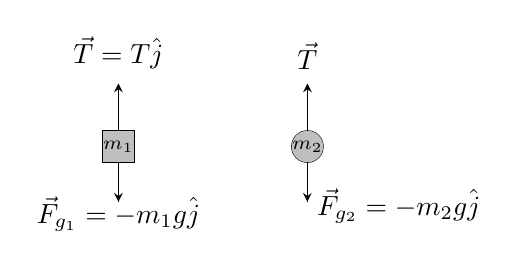
\begin{tikzpicture}
\draw (1.4,1) rectangle (1.8,1.4);
\draw (4,1.2) circle (0.2cm);
\fill[gray!50] (4,1.2) circle (0.2cm);
\fill[gray!50] (1.4,1) rectangle (1.8,1.4);
\node at (1.6, 1.2) {\scriptsize $m_1$};
\node at (4,1.2) {\scriptsize $m_2$};
\draw [->] (1.6,1.4) -- (1.6,2) node [pos = 1.1, above] {$\vec{T} = T\hat{j}$};
\draw [->] (4,1.4) -- (4,2) node [pos = 1.1, above] {$\vec{T}$};
\draw [->] (1.6, 1) -- (1.6,0.5) node [pos = 2, above] {$\vec{F}_{g_1} = -m_1g\hat{j}$};
\draw [->] (4, 1) -- (4,0.5) node [pos = 1.1, right] {$\vec{F}_{g_2} = -m_2g\hat{j}$};
\end{tikzpicture}
\end{center}

Newton's Second Law: 

1D Problem in the $\hat{j}$ direction:
\begin{align*}
  m_1\ddot y_1 &= -m_1g + T \tag{i}\\
  m_s\ddot y_2 &= -m_2g + T \tag{ii}
\end{align*}

Using the constraint 
\[\text{(i) } \implies -m_1 \ddot{y_2} = -m_1g + T\]

Subtract (ii)
\[
\begin{aligned}
  -(m_1 + m_2)\ddot{y_2} &= (m_2 - m_1)g\\
  \implies \Aboxed{\ddot{y_2} &= \frac{m_1 - m_2}{m_1 + m_2}g}
\end{aligned}
\]

We can also find $T$: (i) $\times m_2 + $ (ii) $ \times m_1 \implies$
\[
\begin{aligned}
  0 &= -2m_1m_2g + T(m_1+m_2)\\
  \Aboxed{T &= \frac{2m_1m_2}{(m_1+m_2)}g}
\end{aligned}
\]
\end{example}





\subsubsektion{Use of Intrinsic Coordinates}
We know  $\vec{r}(s)$ or $\vec{r} = x\hat{i} + y(x)\hat{j}$
\begin{enumerate}
  \item $\hat{v} = \frac{d\vec{r}}{ds}$
  \item $\frac{d^2\vec{r}}{ds^2} = \kappa\hat{n}, \kappa = \left|\frac{d^2\vec{r}}{ds^2}\right|, \hat{n} = \frac{1}{\kappa}\frac{d^2\vec{r}}{ds^2}$
\end{enumerate}

Describe acceleration:
\[
  \vec{a} = \ddot{s}\hat{v} + \kappa \dot{s}^2\hat{n}
\]

\begin{center}
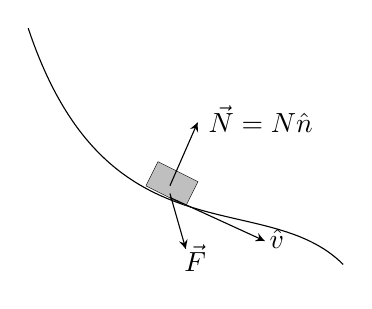
\begin{tikzpicture}
\draw (-1,3) .. controls (0,0) and (2,1) .. (3,0);
\draw (0.5,1) -- (0.65,1.3) -- (1.15,1.05) -- (1,0.75) -- (0.5,1);
\fill[gray!50] (0.5,1) -- (0.65,1.3) -- (1.15,1.05) -- (1,0.75) -- (0.5,1);
\draw [->] (0.8,1) -- (1.15,1.8) node [pos = 1.05, right] {$\vec{N} = N\hat{n}$};
\draw [->] (0.8,0.9) -- (1, 0.2) node [pos = 1.6, above] {$\vec{F}$};
\draw [->] (0.8,0.85) -- (2, 0.3) node [pos = 0.95, right] {$\hat{v}$};
\end{tikzpicture}
\end{center}



From Newton's Second Law:
\[
\begin{aligned}
  m\ddot{s} &= \vec{F}\cdot\hat{v}\\
  m\kappa\dot{s}^2 &= \vec{F}\cdot\hat{n} + N
\end{aligned}
\]~\\

\begin{example}
\begin{center}
	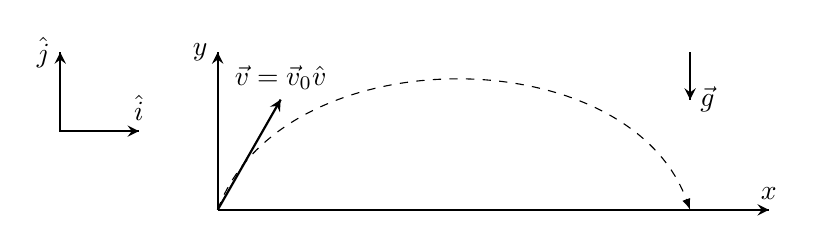
\begin{tikzpicture}[
    media/.style={font={\footnotesize\sffamily}},
    wave/.style={
        decorate,decoration={snake,post length=1.4mm,amplitude=2mm,
        segment length=2mm},thick},
    interface/.style={
        % The border decoration is a path replacing decorator. 
        % For the interface style we want to draw the original path.
        % The postaction option is therefore used to ensure that the
        % border decoration is drawn *after* the original path.
        postaction={draw,decorate,decoration={border,angle=-45,
                    amplitude=0.3cm,segment length=2mm}}},
    ]

    % Interface
    %\draw[blue,line width=.5pt,interface](-5,0)--(4,0);

    % Vertical dashed line
    %\draw[gray](-3,0)--(-3,2);
    
    % Coordinates system
    \draw[->,thick] (-3,0) --(4,0) node[above]{$x$};
    \draw[->,thick] (-3,0) --(-3,2) node[left]{$y$};
    
    % Coordinates system
    \draw[<->,thick] (-4,1) node[above]{$\hat{i}$}-|(-5,2) node[left]{$\hat{j}$};
    
        % Coordinates system
    \draw[->,thick] (3,2)--(3,1.4) node[right]{$\vec{g}$};

        % Coordinates system
    \draw[->,thick] (-3,0)--(-2.2,1.4) node[above]{$\vec{v} = \vec{v}_0\hat{v}$};



    % Interface pointer
    \draw[-latex,dashed](-3,0) to[out=70,in=110] (3,0);
    % To-paths are really useful for drawing curved lines. The above
    % to path is equal to:
    %
    % \draw[-latex,thick](3.2,0.5)node[right]{$\mathsf{S_{1,2}}$}
    %      ..controls +(180:.2cm) and +(up:0.25cm) .. (3,0);
    % Internally the to path is translated to a similar bezier curve,
    % but the to path syntax hides the complexity from the user. 

\end{tikzpicture}
	\end{center}
	
At $t = 0$, $v = \dot{s} = v_0 > 0$ and $x = 0$. 

\emph{For what values of $v_0$ does the object leave the surface before reaching $x = \pi/2$?}

$\implies$ we need to see if the normal force goes to zero. 

\[
\begin{aligned}
  y'(x) &= \cos x, \quad y''(x) = -\sin x\\[0.2cm]
  \hat{v} &= [1+y'^2]^{-1/2}(\hat{i} + y'\hat{j})\\
  &= [1+\cos^2x]^{-1/2}(\hat{i} + \cos x\hat{j})\\[0.2cm]
  \kappa &= \frac{|y''|}{[1+y'^2]^{3/2}} = \frac{\sin x}{[1 + \cos^2x]^{3/2}}\\[0.2cm]
  \hat{n} &= \frac{y''}{|y''|}[1 + y'^2]^{-1/2}[-y'\hat{i} + \hat{j}]\\
  &= -[1+\cos^2x]^{-1/2}[-\cos x \hat{i} + \hat{j}]
\end{aligned}
\]

Force diagram: 
\begin{center}
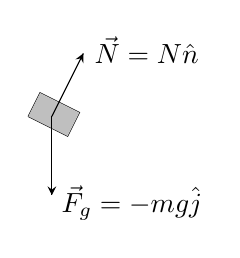
\begin{tikzpicture}
\draw (0.5,1) -- (0.65,1.3) -- (1.15,1.05) -- (1,0.75) -- (0.5,1);
\fill[gray!50] (0.5,1) -- (0.65,1.3) -- (1.15,1.05) -- (1,0.75) -- (0.5,1);
\draw [->] (0.8,1) -- (0.8,0) node [pos = 1.1, right] {$\vec{F}_g = -mg\hat{j}$};
\draw [->] (0.8,1) -- (1.2,1.8) node [pos = 1.05, right] {$\vec{N} = N\hat{n}$};
\end{tikzpicture}	
\end{center}


Newton's Laws: 
\begin{align*}
  m\ddot{s} &= \vec{F}_g \cdot\hat{v}\\
  &= -mg\cos x [1+\cos^2x]^{-1/2} \tag{i}\\
  m\kappa \dot{s}^2 &= \vec{F}_g\cdot\hat{n} + N\\
  &= mg[1 + \cos^2x]^{-1/2} + N \tag{ii}
\end{align*}

Multiply (i) $\times \dot{s}$:

\[
\begin{aligned}
  m\ddot{s}\dot{s} &= -mg[1+\cos^2x]^{-1/2}\cos x \dot{s}\\
  \ddot{s}\dot{s} &= \frac{d}{dt}\left(\frac{\dot{s}^2}{2}\right)\\
  \dot{s} &= \frac{ds}{dx}\dot{x} = [1 + \cos^2x]^{1/2}\dot{x}
\end{aligned}
\]

Substitute these in: 
\[
\begin{aligned}
  m\frac{d}{dt}\left(\frac{\dot{s}^2}{2}\right) &= -mg\cos x \dot{x}\\
  &= -\frac{d}{dt}(g\sin x)\\
  \implies \frac{d}{dt}\left(\frac{\dot{s}^2}{2} + g\sin x\right) &= 0\\
  \implies \frac{\dot{s}^2}{2} + g\sin x &= K
\end{aligned}
\]

Initial conditions: $t = 0, \dot{s} = v_0, x = 0$

$\implies K = v_0^2/2$, $\implies \dot{s}^2 = v_0^2 - 2g\sin x$

Substitute this into $(ii)$
\[
  m \times \frac{\sin x}{[1 + \cos^2x]^{3/2}}(v_0^2 - 2g\sin x) =
  mg[1+\cos^2x]^{-1/2} + N
\]
\[
\begin{aligned}
  N &= \frac{m}{[1+\cos^2x]^{3/2}}(v_0^2\sin x -2g\sin^2x - g(1 + \cos^2x))\\
  N &= \frac{m}{[1+\cos^2x]^{3/2}}[v_0^2\sin x - g(2 + \sin^2x)]
  \end{aligned}
\]~

Set $N = 0$
\[
\begin{aligned}
  \implies &v_0^2\sin x - g(2 + \sin^2x) = 0\\
  &v_0^2 = \frac{g(2 + \sin^2x)}{\sin x}
\end{aligned}
\]

We can show that this has a minimum at $x = \pi/2 \implies v_0^2 = 3g \implies v_0 = \sqrt{3g}$ .

If $v_0 > \sqrt{3g}$ it will leave the surface before reaching $x = \pi/2$. 
\end{example}~

\subsektion{Friction}
  Friction arises  \lecturemarker{14}{22 Oct} when one object is in contact with another: 
  
  \begin{center}
    \begin{tikzpicture}
	\draw (-1,0) -- (6,0); 
	\draw (1.8,2.45) circle (0.3cm);
	\draw (1.8,2.1) -- (1.3,0.8);
	\draw (1.3,0.8) -- (1,0);
	\draw (1.3,0.8) -- (1.6,0);
	\draw (1.7,1.9) -- (2.3,2);
	\draw (2.3,0) rectangle (2.8,2.1);
	\draw [->] (2.5,1.8) -- (4.5,1.8) node [pos = 1.1, right] {$\vec{F}$};
	\draw [->] (2.5,1) -- (1,1) node [pos = 1.1, left] {$\vec{\F}$};    
    \end{tikzpicture}
  \end{center}
 

$\vec{\F}$ is the force due to friction. $|\vec{\F}| < \F_{max}$, friction acts like a constraint force. 

If $|\vec{F}| < \F_{max} \implies \vec{\F} = -\vec{F}$. 

$\F_{max}$ depends on:
\begin{enumerate}
  \item[(a)] The materials of the objects. 
  \item[(b)] The normal force.  
\end{enumerate}

It is independent of the area of contact and velocity. 
\[\F_{max} = \mu|\vec{N}| ~(\mu >0)\]

\begin{definition}
$\mu$ is the \emph{coefficient of friction.}
\end{definition}

Typically $0 < \mu \leq 1$.\\

Once $|\vec{F}| > \F_{max}$: 
\begin{itemize}
  \item The object moves.
  \item $|\vec{\F} = \mu|\vec{N}| = \F_{max}$
  \item Friction opposes the motion of the object.
\end{itemize}\vsp

Before reaching $\F_{max}$ the direction opposes the ``would be'' motion.
Graphically: \vspace*{-20pt}

\begin{center}
\begin{tikzpicture}[scale=.8]
\draw [->] (0,0) -- (6,0) node [pos = 1, right] {$|\vec{F}|$};
\draw [->] (0,0) -- (0,4) node [pos = 1, left] {$|\vec{\F}|$};	
\draw [dashed] (0,3) -- (6,3) node [pos = 1,right] {$\F_{max}$};
\draw (3,3) -- (6,3);
\draw [dashed] (3,3) -- (3,0) node [pos = 1.3,above] {$\F_{max}$};
\draw (0,0) -- (3,3);
\end{tikzpicture}
\end{center}

More generally, $0 \leq |\vec{\F}| \leq \mu|\vec{N}|$. 

\begin{center}
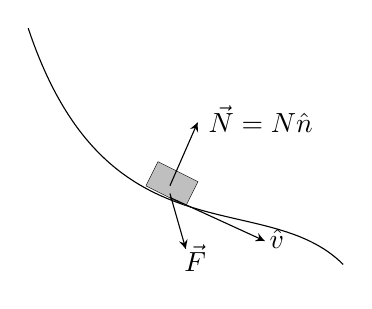
\begin{tikzpicture}
\draw (-1,3) .. controls (0,0) and (2,1) .. (3,0);
\draw (0.5,1) -- (0.65,1.3) -- (1.15,1.05) -- (1,0.75) -- (0.5,1);
\fill[gray!50] (0.5,1) -- (0.65,1.3) -- (1.15,1.05) -- (1,0.75) -- (0.5,1);
\draw [->] (0.8,1) -- (1.15,1.8) node [pos = 1.05, right] {$\vec{N} = N\hat{n}$};
\draw [->] (0.8,0.9) -- (1, 0.2) node [pos = 1.6, above] {$\vec{F}$};
\draw [->] (0.8,0.85) -- (2, 0.3) node [pos = 0.95, right] {$\hat{v}$};
\end{tikzpicture}
\end{center}

There is no relative motion then 
\[\vec{v} = \vec{v}_s \tag{i}\]

Friction works to satisfy (i). 

If there is relative motion, $\vec{v} \neq \vec{v}_s$ and $|\vec{\F}| = \mu|\vec{N}|$ acts to restore (i).

This is an example of a ``mathematical model'' - we can describe the phenomena using mathematics, then use this description to predict other phenomena.\\

 
\begin{example}\vspace*{-10pt}

 \begin{center}
 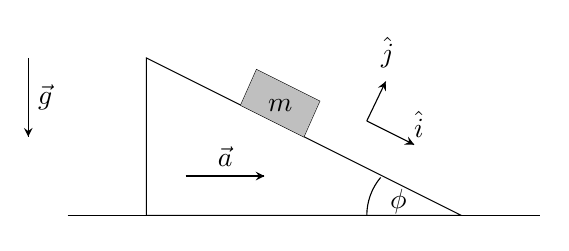
\begin{tikzpicture}
  	\draw (0,0) -- (6,0);
  	\draw (1,0) -- (5,0) -- (1,2) -- (1,0);
  	\draw (3.8, 0) arc (180:140:0.75);
  	\node at (4.2,0.18) {$\phi$};
    \draw (2.2,1.4) -- (3,1) -- (3.2,1.45) -- (2.4, 1.85) -- (2.2,1.4);
    \fill[gray!50] (2.2,1.4) -- (3,1) -- (3.2,1.45) -- (2.4, 1.85) -- (2.2,1.4);
    \draw [->] (3.8,1.2) -- (4.04,1.7) node [pos = 1.1, above] {$\hat{j}$};
    \draw [->] (3.8,1.2) -- (4.4,0.9) node [pos = 1.1, above] {$\hat{i}$};
    \node at (2.7,1.4) {$m$};
    \draw [->] (-0.5,2) -- (-0.5,1) node [pos = 0.5, right] {$\vec{g}$};
    \draw [->] (1.5,0.5) -- (2.5,0.5) node [pos = 0.5, above] {$\vec{a}$};
  \end{tikzpicture}
  \end{center}
  
  
\emph{At what value of $\phi$ does the block begin to slide?}
$\implies$ Friction acting like a constraint. 

Force diagram:\vspace*{-10pt}
\begin{center}
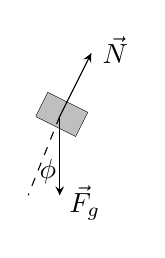
\begin{tikzpicture}
\draw (0.5,1) -- (0.65,1.3) -- (1.15,1.05) -- (1,0.75) -- (0.5,1);
\fill[gray!50] (0.5,1) -- (0.65,1.3) -- (1.15,1.05) -- (1,0.75) -- (0.5,1);
\draw [->] (0.8,1) -- (0.8,0) node [pos = 1.1, right] {$\vec{F}_g$};
\draw [dashed] (0.8,1) -- (0.4,0);
\draw [->] (0.8,1) -- (1.2,1.8) node [pos = 1.05, right] {$\vec{N}$};
\node at (0.65,0.3) {$\phi$};
\end{tikzpicture}	
\end{center}


Since there is no relative motion $\vec{v} = \vec{v}_s = 0$, $\dot{y} = \ddot{y} = \dot{x} = \ddot{x} = 0$

No acceleration, we have static equilibrium. Newton's Second Law;
\begin{align*}
m\ddot{x} &= 0 = mg\sin\phi - \mathfrak{F} \tag{i}\\	
m\ddot{y} &= 0 = -mg\cos\phi + N \tag{ii}\\
\implies N &= mg\cos\phi\\
 \mathfrak{F} &= mg\sin\phi 
\end{align*}

We also know 
\[\mathfrak{F} \leq \mu N = \mu mg\cos\phi\]
Also have 
\[\mathfrak{F} = mg\sin\phi \leq \mu mg \cos\phi\]
or 
\[\mu \geq \tan\phi\] 
Thanks Euler!

So when $\mathfrak{F} = \mathfrak{F}_{max}$
\[\implies \mu = \tan\phi\]
For $\mu < \tan\phi$ the object is moving in the $\hat{i}$ direction and $\ddot{x} \neq 0$. 

Newton's Second Law
\[
\begin{aligned}
m\ddot{x} &= mg\sin\phi - \mathfrak{F}_{max}\\
&= mg\sin\phi - \mu mg\cos\phi \\
\implies \ddot{x} &= g[\sin\phi - \mu\cos\phi]	
\end{aligned}
\]
\end{example}

\subsektion{Drag Force}

Example \lecturemarker{15}{22 Oct} of a force that depends on the velocity of an object. 

Motion of bodies through fluid. 
\begin{center}
\begin{tikzpicture}[scale = 0.7]
	\draw (0,0) circle (1.5cm);
	\draw [->] (0,0) -- (3,2) node [pos = 1.05, right] {$\vec{v} = v\hat{v}$};
	\draw [->] (2,2.5) to[out=240,in=0] (1,2);
	\draw [->] (-1,2) to[out=210,in=70]  (-2,1.5);
	\draw [<-] (1,-2) to[out=20, in=180] (2,-1.5);
	\draw [->] (-1,-2) to[out =200, in = 100] (-1.5,-2.8);
	\draw [->] (-2.2,0) to[out = 270, in = 10] (-2.6,-1);
\end{tikzpicture}	
\end{center}

Fluid has: $\rho$: density and $\eta$: viscosity

To move through the fluid, the body exerts a force on the fluid: $\vec{F}_{FB}$

By Newton's III Law
\[\vec{F}_{BF} = -\vec{F}_{FB}\]
The drag force \[\vec{F}_D = (\vec{F}_{BF}\cdot \hat{v})\hat{v}\]

In general to find $\vec{F}_{D}$ is a challenging problem! To find $\vec{u}$ we need to solve the Navier-Stokes Equations. From $\vec{u}$ we can obtain $\vec{F}_D$. Fortunately this calculation can be done for two limiting cases; at low and at high speeds:

\subsubsektion{Low Speeds}
At low speeds $|\vec{v}| << 1$, then 
\[\vec{F}_D = -C_D\vec{v}\]
Where $C_D$ is the \emph{drag co-efficient}

\begin{itemize}
\item This depends linearly on $\vec{v}$.
\item Always opposite the direction of motion
\item For a sphere $C_D = 6\pi R\eta$
\item $C_D$ depends on (i) the size of the object, (ii) the viscosity of the fluid
\end{itemize}
If $\vec{u} \neq 0$ meaning there is a background flow:
\[\vec{F}_D = -C_D(\vec{v} - \vec{u})\]
only a drag force if there's relative motion to the fluid.\\

\subsubsektion{High Speeds}
\[\vec{F}_D = -C_D|\vec{v}|\vec{v}\]
\begin{itemize}
\item Opposes the motion
\item Depends quadratically on the speed
\item Changes $C_D = \frac{1}{2}\rho R^2K$
\item Drag Force is not all of $\vec{F}_{BF}$
\begin{center}
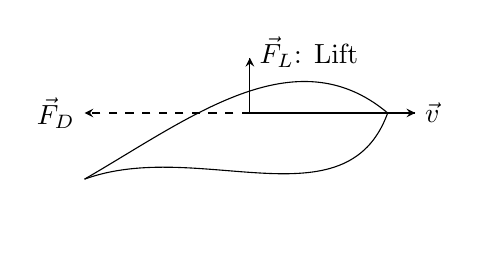
\begin{tikzpicture}[scale=.7]
\draw [->] (0,0) -- (3,0) node [pos = 1, right] {$\vec{v}$};
\draw [->] (0,0) -- (0,1) node [pos = 1.1, right] {$\vec{F}_L$: Lift};
\draw [->, dashed] (0,0) -- (-3,0) node [pos = 1,left] {$\vec{F}_D$};
\draw (-3,-1.2) to[out=30,in=140] (2.5,0); 
\draw (-3,-1.2) to[out=20, in=250] (2.5,0);
\end{tikzpicture}
	
\end{center}
\end{itemize}


\begin{example}
\begin{center}
\begin{tikzpicture}
\draw[<->,line width=1pt] (5,0) node[above]{$\hat{i}$}-|(4,1) node[left]{$\hat{j}$};
\fill (0,0) circle (2pt);
\draw[->] (0,0) -- (1,1) node [pos = 1,right] {$\vec{v}$};
\draw[->] (2,1) -- (2,0) node [pos = 1,right] {$\vec{g}$};
\end{tikzpicture}
\end{center}

$\vec{F}_D = -C_D\vec{v}$

Force Diagram:

\begin{center}
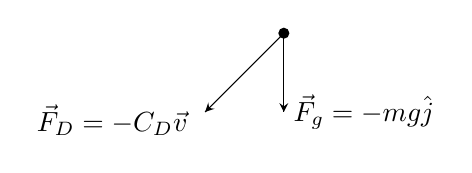
\begin{tikzpicture}
	\fill (0,0) circle (2pt);
	\draw [->] (0,0) -- (-1,-1) node [pos = 1.1,left] {$\vec{F}_D = -C_D\vec{v}$};
	\draw [->] (0,0) -- (0,-1) node [pos = 1, right] {$\vec{F}_g = -mg\hat{j}$};
\end{tikzpicture}	
\end{center}


Newton's Second Law:
\[m\frac{d\vec{v}}{dt} = \vec{F}_D + \vec{F}_g = -C_D\vec{v} - mg\hat{j}\]

First, seek the solution, $\vec{v}_{\infty}$, where $\dfrac{d\vec{v}}{dt} = 0$, the \emph{steady state solution}

\[
\begin{aligned}
\implies 0 &=  -C_D\vec{v} - mg\\
\implies \vec{v}_{\infty} &= -\frac{mg}{C_D}\hat{j}
\end{aligned}\]

Using linearity of the equation
\[\vec{v} = \vec{v}_{\infty} + \vec{w}\]

Substitute this into Newton's Second Law:
\[\begin{aligned}
m\frac{d}{dt}(\vec{v}_{\infty} + \vec{w}) &= -C_D(\vec{v}_{\infty} + \vec{W}) - mg\hat{j}\\
m\frac{d\vec{w}}{dt} &= mg\hat{j} -C_D\vec{w} - mg\hat{j}\\
\implies \frac{d\vec{w}}{dt} &= -\frac{C_D}{m}\vec{w} \\
\implies \vec{w} &= \vec{w}_0e^{-C_Dt/m}
\end{aligned}\]

Thus 
\[\vec{v} = -\frac{mg}{C_D}\hat{j} + \vec{w}_0e^{-C_Dt/m}\]

Initial condition: $t= 0$, $\vec{v} = \vec{v}_0 \implies \vec{w}_0 = \vec{v}_0 + \frac{mg}{C_D}\hat{j}$. So
\[\vec{v} = \vec{v}_0e^{-C_Dt/m} - \frac{mg}{C_D}\hat{j}[1-e^{-C_Dt/m}]\]

As $t \to \infty$, $\vec{v} \to -\frac{mg}{C_D}\hat{j} = \vec{v}_{\infty}$ as expected.

The ratio $C_D/m$ controls how quickly this limit is reached. 

Taking $\vec{v}_0 = 0$
\[\vec{v} = -\frac{mg}{C_D}\hat{j}[1 - e^{-C_Dt/m}]\]
\begin{center}
\begin{tikzpicture}[scale=.8]
\draw [->] (0,0) -- (7,0) node [pos = 1,right] {$t$};
\draw [->] (0,-2) -- (0,2) node [pos = 1,left] {$v_y$};	
\draw [dashed] (0,-1.2) -- (7,-1.2) node [pos = 1, right] {$mg/C_D$};
\draw (0,0) to[out = 300, in = 180] (2,-1.18);
\draw (2,-1.18) -- (7,-1.19);
\end{tikzpicture}
	
\end{center}


Integrating our general expression to find the position:
\[\vec{r}(t) = \vec{r}_0 - \frac{mgt}{C_D}\hat{j} + \frac{m}{C_D}[\vec{v}_0 + \frac{mg}{C_D}\hat{j}]\times(1-e^{-C_Dt/m})\]
\end{example}


\textbf{Projectiles:} $\vec{r}_0 = 0$, $\vec{v}_0 = v_0\cos\alpha\hat{i} + v_0\sin\alpha\hat{j}$\\[4cm]

\begin{center}
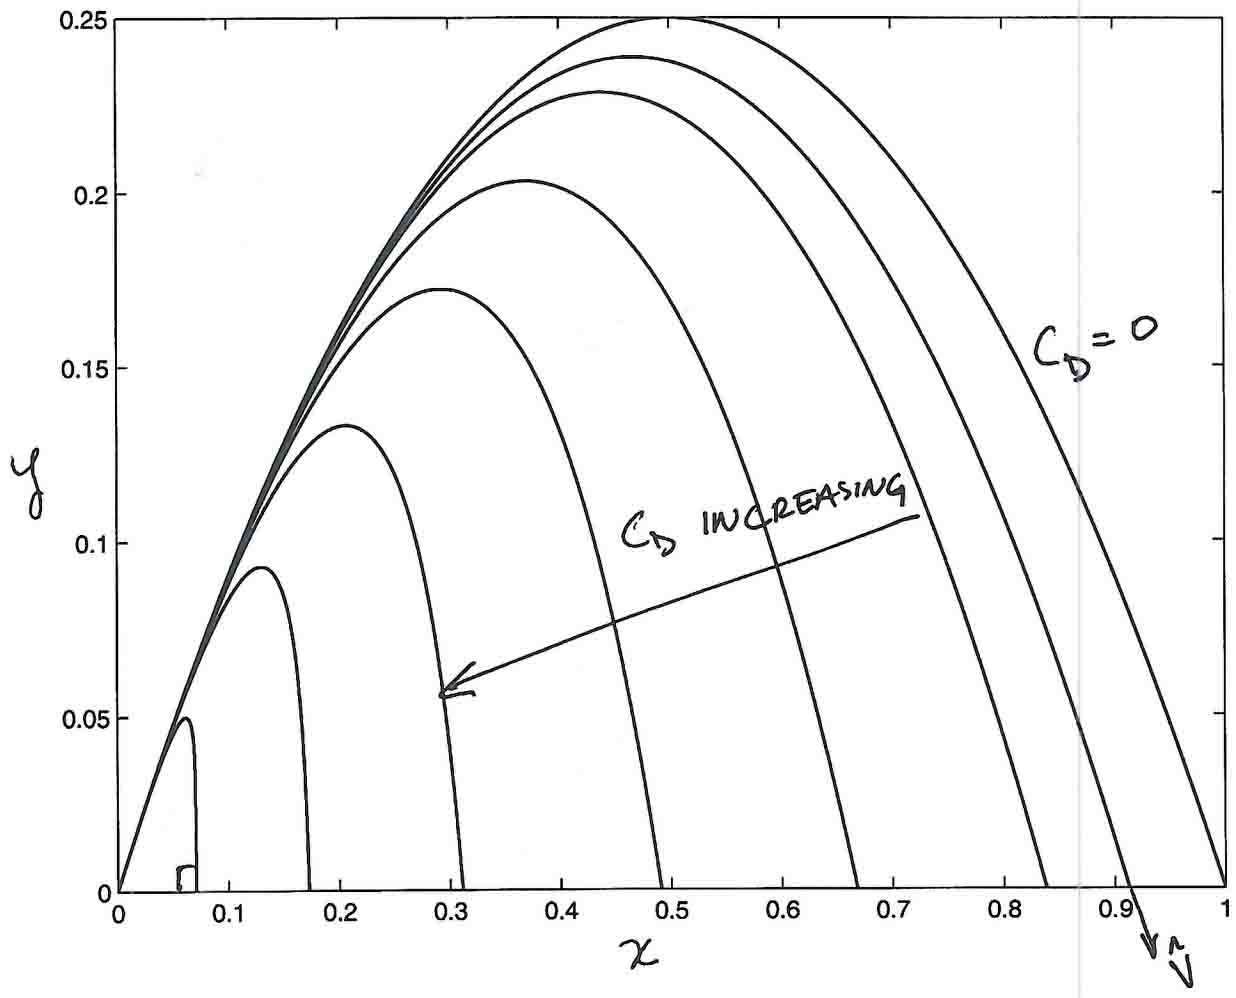
\includegraphics[width=4cm]{drag.jpg}
\end{center}




\sektion{Oscillators}

1660: Ceiiinosssttuv \lecturemarker{16}{22 Oct}

1678: ``Ut tensio sic vis'', ``As is the extension, so the force'' - Robert Hooke

\subsektion{Spring Force}

\begin{itemize}
  \item Example of a force that depends on position
  \item Spring forces are related to the deformations of solids
\end{itemize}



\begin{center}
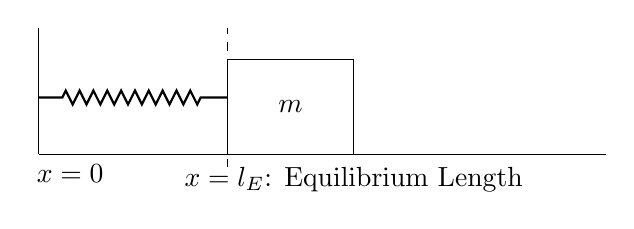
\begin{tikzpicture}[scale=.8]
 \tikzstyle{spring}=[thick,decorate,decoration={zigzag,pre length=0.3cm,post
 length=0.3cm,segment length=5}]
 \tikzstyle{ground}=[fill,pattern=north east lines,draw=none,minimum
 width=0.75cm,minimum height=0.3cm]
\draw (0,0) -- (9,0);
\draw (3,0) rectangle (5,1.5) node [pos = 0.5] {$m$};
\draw (0,0) -- (0,2);
\draw[spring] (0,0.9) -- (3,0.9);
\node at (0.5,-0.3) {$x = 0$};
\draw [dashed] (3,-0.2) -- (3,2) node at (5,-0.4) {$x = l_E$: Equilibrium Length};
\end{tikzpicture}
\end{center}

\begin{center}
\begin{tikzpicture}[scale=.8]
 \tikzstyle{spring}=[thick,decorate,decoration={zigzag,pre length=0.3cm,post
 length=0.3cm,segment length=6}]
 \tikzstyle{ground}=[fill,pattern=north east lines,draw=none,minimum
 width=0.75cm,minimum height=0.3cm]
\draw (0,0) -- (9,0);
\draw (4.5,0) rectangle (6.5,1.5) node [pos = 0.5] {$m$};
\draw (0,0) -- (0,2);
\draw[spring] (0,0.9) -- (4.5,0.9);
\draw [dashed] (3,-0.2) -- (3,2) node at (3.8,2) {$\Delta x$};
\draw [->] (6,0.6) -- (7.5,0.6) node [pos = 1,right] {$\vec{F}$};
\end{tikzpicture}
\end{center}

\begin{center}
\hspace*{0.6cm}
\begin{tikzpicture}[scale=.8]
 \tikzstyle{spring}=[thick,decorate,decoration={zigzag,pre length=0.3cm,post
 length=0.3cm,segment length=7}]
 \tikzstyle{ground}=[fill,pattern=north east lines,draw=none,minimum
 width=0.75cm,minimum height=0.3cm]
\draw (0,0) -- (9,0);
\draw (6,0) rectangle (8,1.5) node [pos = 0.5] {$m$};
\draw (0,0) -- (0,2);
\draw[spring] (0,0.9) -- (6,0.9);
\draw [dashed] (3,-0.2) -- (3,2) node at (3.8,2) {$\Delta x$};
\draw [dashed] (4.5,-0.2) -- (4.5,2) node at (5.2,2)  {$\Delta x$};
\draw [->] (7.5,0.6) -- (9,0.6) node [pos = 1,right] {$2\vec{F}$};
\end{tikzpicture}
\end{center}

There is a linear relationship between $|\vec{F}|$ and $\Delta x$:

\begin{center}
\begin{tikzpicture}[scale=.8]
\draw [->] (0,0) -- (6,0) node [pos = 1, right] {$\Delta x$};
\draw [->] (0,0) -- (0,4) node [pos = 1, left] {$|\vec{F}|$};	
\draw [dashed] (3,3) -- (3,2) node [pos = 0.5,right] {$k$};
\draw [dashed] (3,2) -- (2,2) node [pos = 0.5, below] {$1$};
\draw (0,0) -- (3.5,3.5);
\node at (5,2) {$|\vec{F}| = k\Delta x$};
\end{tikzpicture}
\end{center}

 
\begin{definition}
$k$ is the \emph{spring constant}. 
\end{definition}

$k$ depends on:
\begin{enumerate}
  \item Material
  \item Geometry of the spring 
\end{enumerate}

The spring acts in a way to restore its equilibrium length.

\begin{center}
\hspace*{0.6cm}
\begin{tikzpicture}[scale=.8]
 \tikzstyle{spring}=[thick,decorate,decoration={zigzag,pre length=0.3cm,post
 length=0.3cm,segment length=6}]
 \tikzstyle{ground}=[fill,pattern=north east lines,draw=none,minimum
 width=0.75cm,minimum height=0.3cm]
\draw (0,0) -- (9,0);
\draw (6,0) rectangle (8,1.5) node [pos = 0.5] {$m$};
\node at (6,-0.4) {$x$};
\draw (0,0) -- (0,2);
\draw[spring] (0,0.9) -- (6,0.9);
\draw [dashed] (3,-0.2) -- (3,2) node [pos = 0,below] {$l_E$};
\draw [->] (6.5,1.8) -- (5,1.8) node [pos = 0.5, above] {$\vec{F}_s$ in $\hat{i}$ direction};
\end{tikzpicture}
$|\vec{F}_s| = k(x-l_E)$
\end{center}



\begin{center}
\hspace*{0.6cm}
\begin{tikzpicture}[scale=.8]
 \tikzstyle{spring}=[thick,decorate,decoration={zigzag,pre length=0.1cm,post
 length=0.1cm,segment length=3}]
 \tikzstyle{ground}=[fill,pattern=north east lines,draw=none,minimum
 width=0.75cm,minimum height=0.3cm]
\draw (0,0) -- (9,0);
\draw (2,0) rectangle (4,1.5) node [pos = 0.5] {$m$};
\node at (2,-0.3) {$x$};
\draw (0,0) -- (0,2);
\draw[spring] (0,0.9) -- (2,0.9);
\draw [dashed] (5.5,-0.2) -- (5.5,2) node [pos = 0,below] {$l_E$};
\draw [->] (3.5,0.6) -- (4.5,0.6) node [pos = 1,right] {$\vec{F}_s$ in $\hat{i}$};
\end{tikzpicture}
$|\vec{F}_s| = k(l_E-x)$
\end{center}



The spring force
\[\vec{F}_s = -k(x-l_E)\hat{i}\]

If $l_E = 0$
\[\vec{F}_s = -kx\hat{i}\]

In 3D: 
\[\vec{F}_s = -k(\vec{r} - \vec{r}_E)\]

If $\vec{r}_E = 0$
\[\vec{F}_s = -k\vec{r}\]

\begin{center}
\hspace*{0.6cm}
\begin{tikzpicture}[scale=.8]
 \tikzstyle{spring}=[thick,decorate,decoration={zigzag,pre length=0.3cm,post
 length=0.3cm,segment length=6}]
 \tikzstyle{ground}=[fill,pattern=north east lines,draw=none,minimum
 width=0.75cm,minimum height=0.3cm]
\draw (0,0) -- (9,0);
\draw (6,0) rectangle (8,1.5) node [pos = 0.5] {$m$};
\node at (6,-0.4) {$x_0$};
\node at (1.5,0.3) {Frictionless};
\draw (0,0) -- (0,2);
\draw[spring] (0,0.9) -- (6,0.9);
\draw [dashed] (3.5,-0.2) -- (3.5,2) node [pos = 0,below] {$x = 0$};
\draw [->] (6.5,1.8) -- (5,1.8) node [pos = 1, above] {$\vec{F}_s$};
\end{tikzpicture}
\end{center}

We only need to worry about the spring force (other forces balance). Newton's Second Law 
\[m\ddot{x} = -kx ~(*)\]
We seek a solution of the form $x = Ce^{\alpha t}$, $\dot{x} = C\alpha e^{\alpha t}$, $\ddot{x} = C\alpha^2 e^{\alpha t}$. Substituting this into $(*)$
\[
\begin{aligned}
  m[C\alpha^2e^{\alpha t}] &= -kCe^{\alpha t}\\
  Ce^{\alpha t}[m\alpha^2 + k] &= 0\\
  \implies \alpha^2 &= -\frac{k}{m}\\
  \alpha &= \pm i\sqrt{\frac{k}{m}}
\end{aligned}
\]
The general solution is 
\[x(t) = C_1e^{i\sqrt{k/m}t} + C_2e^{-i\sqrt{k/m}t}\]

$x$ is real but $C_1$ and $C_2$ are complex. The equivalent general solution is 

\[
\begin{aligned}
  x(t) &= C_3\cos\sqrt{k/m}t + C_4\sin\sqrt{k/m}t\\
  \dot{x}(t) &= -C_3\sqrt{k/m}\sin\sqrt{k/m}t + C_4\sqrt{k/m}\cos\sqrt{k/m}t
\end{aligned}
\]

Initial conditions:
\[t = 0,~\dot{x} = 0 \implies C_4 = 0\]
\[t = 0,~x - x_0 \implies C_3 = x_0\]

So the solution is 
\[x(t) = x_0\cos\sqrt{\frac{k}{m}}t\vspace*{-10pt}\]
  \begin{center}
    \begin{tikzpicture}[scale=.7]
      \draw [domain=-2:2] plot ({2*\x}, {-2 * cos(90 * \x)});
      \draw [->] (-4, 0) -- (4.5, 0) node [right] {$t$};
      \draw [->] (-4, -2.5) -- (-4, 2.5) node [above] {$x(t)$};
      \draw [dashed] (-4,2) -- (4,2) node [pos =0,left] {$x_0$}; 
      \draw [dashed] (-4,-2) -- (4,-2) node [pos=0,left] {$-x_0$};
      \draw [dashed] (-2, 2) -- (-2, -2) node [below] {$T_0/4$};
      \draw [dashed] (2, 2) -- (2, -2) node [below] {$3T_0/4$};
      \draw [dashed] (0, 2) -- (0, -2) node [below] {$T_0/2$};
      \draw [dashed] (4, 2) -- (4, -2) node [below] {$T_0$};
    \end{tikzpicture}
  \end{center}
  
$x(t)$ has:
\begin{itemize}
  \item Amplitude of oscillation $A = x_0$
  \item Period $T_0 = 2\pi\sqrt{\frac{m}{k}}$
  \item Frequency: $\omega_0 = \sqrt{\frac{k}{m}} \implies \omega_0 = \frac{2\pi}{T_0}$
\end{itemize}

Amplitude just depends on the initial conditions. The frequency depends solely on $k$ \& $m$. This system is an example of a \emph{simple harmonic oscillator}.\\

 Similar equations arises with a pendulum:
\begin{center}
\begin{tikzpicture}
      \draw (-1, 0) -- (1, 0);
      \draw [ultra thick] (0, 0) -- (1, -2) node [anchor = south west, pos = 0.5] {$\ell$};
      \draw [dashed] (0, 0) -- (0, -2.5);
      \draw [->] (0.5, -1) -- (0.5, -2) node [below] {$Mg$};
      \draw[<->,line width=1pt] (5,-1) node[above]{$\hat{i}$}-|(4,-2) node[left]{$\hat{j}$};
\end{tikzpicture}
\end{center}

Newton's Second Law:
\[
\begin{aligned}
  m(\ddot{r} - r\dot{\theta}) &= mg\cos\theta - T\\
  m(r\ddot{\theta} + 2\dot{r}\dot{\theta}) &= -mg\sin\theta\\
\end{aligned}
\]

Since $r = l$, $\dot{r} = \ddot{r} = 0$:
\[
\begin{aligned}
  \implies -ml\dot{\theta}^2 &= mg\cos\theta - T\\
  ml\ddot{\theta} &= -mg\sin\theta 
\end{aligned}
\]

If the angle $\theta$ remains small, $\theta << 1$, $\sin\theta \approx \theta$. When we do this 
\[
\begin{aligned}
  ml\ddot{\theta} &= -mg\theta\\
  \implies \ddot{\theta} + \frac{g}{l}\theta &= 0 
\end{aligned}
\]

This is the same as our equation for the spring with 
\[
\begin{aligned}
  x &\longrightarrow \theta\\
  \frac{k}{m} &\longrightarrow \frac{g}{l}
\end{aligned}
\]

For a pendulum $\omega_0 = \sqrt{\frac{g}{l}}$. 


\subsektion{Damped Harmonic Oscillator} 

\begin{center}\lecturemarker{17}{22 Oct}
\begin{tikzpicture}[scale=.8]
 \tikzstyle{spring}=[thick,decorate,decoration={zigzag,pre length=0.3cm,post
 length=0.3cm,segment length=6}]
 \tikzstyle{ground}=[fill,pattern=north east lines,draw=none,minimum
 width=0.75cm,minimum height=0.3cm]

\draw (0,0) -- (8,0);
\draw (5,0) rectangle (7,1.5) node [pos = 0.5] {$m$};
\draw (0,0) -- (0,2.5);
\draw[spring] (0,0.9) -- (5,0.9)node [midway,above] {$k$};
\draw [dashed] (3.5,0) -- (3.5,2.5) node [pos = 0,below] {$x = 0$};
\draw [->] (5.5,0.6) -- (4,0.6) node [pos = 0.9, below] {$\vec{v}$};
\draw [->] (6.5,0.6) -- (8,0.6) node [pos = 1,right] {$\vec{F}_D$};
\draw [->] (5.5,1.9) -- (4,1.9) node [pos = 0.9, above] {$\vec{F}_s$};
\end{tikzpicture}
\end{center}

Take: $\vec{F}_D = -C_D\vec{v}$. Motion is still 1D! 

Newton's Second Law:
\[
\begin{aligned}
  m\ddot{x} &= -kx -C_D\dot{x}\\
  \ddot{x} + \frac{C_D}{m}\dot{x} + \frac{k}{m}x &= 0
\end{aligned}
\]

Recall: $\omega_0^2 = \frac{k}{m}$, $\mu= \frac{C_D}{2m}$
\[\ddot{x} + 2\mu\dot{x} + \omega_0^2x = 0 \tag{$*$}\]

Look for a solution of the form $x = Ce^{\alpha t}$. Plug this into ($*$):
\[Ce^{\alpha t}[\alpha^2 + 2\mu\alpha + \omega_0^2] = 0\]

Solving our quadratic equation for $\alpha$
\[\alpha = \frac{-2\mu \pm \sqrt{4\mu^2 -4\omega_0^2}}{2}\]

Two solutions:
\[
\begin{aligned}
  \alpha_1 = -\mu + \sqrt{\mu^2 -\omega_0^2}\\
  \alpha_2 = -\mu -\sqrt{\mu^2 -\omega_0^2}
\end{aligned}
\]

The general solution is
\[x(t) = C_1e^{\alpha_1t} + C_2e^{\alpha_2t}\]

We know that both $\mu, \omega_0 >0$, but there are three cases to consider:

\begin{enumerate}
  \item $\mu > \omega_0$: Over damped
  \item $\mu < \omega_0$: Under damped
  \item $\mu = \omega_0$: Critically damped
\end{enumerate}~

\textbf{Case (i):}

$\mu^2 - \omega_0^2 > 0$

$\implies \alpha_1$ and $\alpha_2$ are real. We also know $\mu > \sqrt{\mu^2 - \omega_0^2} \implies$ both $\alpha_1,\alpha_2 < 0$. 

Our solutions decay exponentially to zero.\\

\textbf{Case (ii):}
\[
\begin{aligned}
\mu < \omega_0
  \implies \mu^2 &- \omega_0^2 < 0\\
  \implies \alpha_1 &= -\mu + i\sqrt{\omega_0^2 -\mu^2}\\
  \alpha_2 &= -\mu -i\sqrt{\omega_0^2 - \mu^2}
\end{aligned}
\]
$\implies \alpha_1$ and $\alpha_2$ are complex and in fact complex conjugates of one another. 

General solution:
\[
\begin{aligned}
  x(t) &= C_1e^{-\mu + i\omega_D)t} + C_2e^{-\mu-i\omega_D)t}\\
  \omega_D &= \sqrt{\omega_0^2 - \mu^2}\\
  x(t) &= e^{-\mu t}[C_1e^{i\omega_Dt} + C_2e^{-\omega_Dt}]
\end{aligned}
\]

\begin{itemize}
  \item Drag force modifies the frequency: $\omega_D < \omega_0$
  \item Amplitude decays with time. 
  \item $x(t)$ still goes to zero at $t \to \infty$.
\end{itemize}~


\textbf{Case (iii):}
\[\mu = \omega_0 \implies \alpha_1 = \alpha_2 = -\mu\]

Rethink the general solution:
\[x(t) = C_1e^{-\mu t} + C_2te^{-\mu t}\]

\begin{itemize}
  \item No oscillations
  \item $x \to 0$ as $t \to \infty$. This happens more rapidly than any solution in case (i). 
\end{itemize}~


\begin{example}

$\dot{x} = 0, x(0) = L$. $\mu < \omega_0 \implies$ under damped.

The general solution:
\[
\begin{aligned}
  x(t) &= e^{-\mu t}[K_1\cos\omega_Dt + K_2\sin\omega_Dt]\\
  \dot{x}(t) &= \mu e^{-\mu t}[K_1\cos\omega_Dt + K_2\sin\omega_Dt] + \omega_De^{-\mu t}[-K_1\sin\omega_Dt + K_2\cos\omega_Dt]
\end{aligned}
\]

Apply the initial conditions:
\[
\begin{aligned}
  x(0) &= L = K_1\\
  \dot{x}(0) &= 0\\
  \implies &-\mu L  + \omega_DK_2 = 0\\
 \implies K_2 &= \frac{\mu L}{\omega_D}
\end{aligned}
\]

Solution: 
\[x(t) = Le^{-\mu t}\left[\cos\omega_Dt + \frac{\mu}{\omega_D}[\sin\omega_Dt\right]\]	
\end{example}

We can also express the general solution using an \emph{amplitude} and a \emph{phase}:
\[
\begin{aligned}
  x(t) &= \underbrace{A(t)}_{\text{Amplitude}}\cos(\omega_Dt - \underbrace{\phi)}_{\text{Phase}}\\
  x(t) &= A(t)[\cos\omega_Dt\cos\phi + \sin\omega_Dt\sin\phi]\\
  &= [A(t)\cos\phi]\cos\omega_Dt + [A(t)\sin\phi]\sin\omega_Dt
\end{aligned}
\]

By comparing with our previous expression for the general solution:
\[
\begin{aligned}
  A(t)\cos\phi &= K_1e^{-\mu t}\\
  A(t)\sin\phi &= K_2e^{-\mu t}\\
  \implies \tan\phi &= K_2/K_1\\
  A &= e^{-\mu t}[K_1^2 + K_2^2]^{1/2}
\end{aligned}
\]

For our example $K_1 = L, K_2 = \frac{\mu L}{\omega_D}$
\[
\begin{aligned}
  \tan\phi &= \mu/\omega_D\\
  A &= e^{-\mu t}\left[L^2 + \frac{\mu^2L^2}{\omega_D^2}\right]^{1/2}
\end{aligned}
\]

As $t \to \infty, A \to 0$. 

We see in this case \emph{without} any external forcing that the amplitude and phase depend on the initial conditions.




\subsektion{Forced, Damped Oscillator} 
\begin{center}\lecturemarker{18}{22 Oct}
\begin{tikzpicture}[scale=.8]
 \tikzstyle{spring}=[thick,decorate,decoration={zigzag,pre length=0.3cm,post
 length=0.3cm,segment length=6}]
 \tikzstyle{ground}=[fill,pattern=north east lines,draw=none,minimum
 width=0.75cm,minimum height=0.3cm]

\draw (0,0) -- (8,0);
\draw (5,0) rectangle (7,1.5) node [pos = 0.5] {$m$};
\draw (0,0) -- (0,2.2);
\draw[spring] (0,0.9) -- (5,0.9)node [midway,above] {$k$};
\draw [->] (6.5,0.6) -- (8,0.6) node [pos = 1,right] {$\vec{F}(t)$};
\node at (6,1.8) {$C_D$};
\end{tikzpicture}
\end{center}
\[F(t) = F_0\cos\omega t\]

In general  $\omega \neq \omega_0 \neq \omega_D$. 

Newton's Laws
\[m\ddot{x} = -kx - C_D\dot{x} + F_0\cos\omega t\] 

Using $\mu = C_D/2m$, $\omega^2 = k/m$
\[\ddot{x} + 2\mu\dot{x} + \omega_0^2x = \frac{F_0}{m}\cos\omega t \tag{*}\]

Inhomogeneous equation
\[x(t) = x_{CF}(t) + x_{PI}(t)\]

We know $x_{CF}$ from looking at the damped harmonic oscillator. To find $x_{PI}(t)$ let's look for solutions of the form
\[
\begin{aligned}
  x_{PI}(t) &= K_3\cos\omega t + K_4\sin\omega t\\
  \dot{x}_{PI} &= -K_3\omega\sin\omega t + K_4\omega\cos\omega t\\
  \ddot{x}_{PI} &= -K_3\omega^2\cos\omega t -K_4\omega^2\sin\omega t
\end{aligned}
\]

Plus this all into $(*)$
\[
\begin{aligned}
  &[-K_3\omega^2 + 2\mu\omega K_4 + K_3\omega_0^2 - \frac{F_0}{m}]\cos\omega t\\
  + &[-K_4\omega^2 - 2\mu\omega K_4 + K_4\omega_0^2]\sin\omega t = 0
\end{aligned}
\]

Only possible if everything in the brackets is zero! 
\[
\begin{aligned}
  \implies 2\mu\omega K_4 &= K_3(\omega^2 - \omega_0^2) + \frac{F_0}{m}\\
  2\mu\omega K_3 &= -K_4(\omega^2 - \omega_0^2)
\end{aligned}
\]

Solving for $K_3$ \& $K_4$

\[
\begin{aligned}
   K_3 &= -\frac{F_0}{m}\frac{\omega^2 - \omega_0^2}{4\mu^2\omega^2 + (\omega^2 - \omega_0^2)^2}\\
   K_4 &= \frac{F_0}{m}\frac{2\mu\omega}{4\mu^2\omega^2 + (\omega^2 - \omega_0^2)^2}  
\end{aligned}
\]

The complete general solution:
\[x(t) = K_1e^{\alpha_1t} + K_2e^{\alpha_2t} + K_3\cos\omega t + K_4\sin\omega t\]

As $t \to \infty$, $x_{CF}(t) \to 0$, but $x_{PI}(t)$ does not. 

\[x(t) \to K_3\cos\omega t + K_4\sin\omega t\]

Write the steady state solution as 

\[x(t) \to A\cos[\omega t - \phi]\]

We know from yesterday 

\[A = [K_3^2 + K_4^2]^{1/2},~\tan\phi = K_4/K_3\]

\[
\begin{aligned}
A &= [K_3^2 + K_4^2]^{1/2}\\
\tan\phi &= K_4/K_3\\
  A &= \frac{F_0}{m} \frac{1}{[4\mu^2\omega^2 + (\omega^2 - \omega_0^2)^2]^{1/2}}\\
  \tan\phi &= -\frac{2\mu\omega}{\omega^2-\omega_0^2}
\end{aligned}
\]

Since this is the steady state, for this case $A$ \& $\phi$ are independent of the initial conditions.\\

\textbf{Amplitude:}
\begin{itemize}
  \item $\omega = 0$
  
  $ \implies A(\omega = 0) = \dfrac{F_0}{m}\dfrac{1}{\omega_0^2} = A_0$
  \item $\omega \to \infty$. 
  
  A decays like $\omega^{-2} \implies A \to 0$
\end{itemize}

\emph{What happens in between?} Look at $\dfrac{dA}{d\omega}$

\[\frac{dA}{d\omega} = -\frac{F_0}{m}\frac{8\mu^2\omega + 4(\omega^2-\omega_0^2)\omega}{[4\mu^2\omega^2 + (\omega^2-\omega_0^2)^2]^{3/2}}\]

Find where $\dfrac{dA}{d\omega} = 0$
\begin{itemize}
  \item $\dfrac{dA}{d\omega} \to 0$ as $\omega \to \infty$
  \item Consider the numerator:
  \[
\begin{aligned}
  4\omega[2\mu^2 + (\omega^2 - \omega_0^2)] = 0\\
  \implies \omega = 0 \text{ \& } \omega^2 = \omega_0^2 - 2\mu^2 \equiv \omega_R^2
\end{aligned}
\]

\end{itemize}

\begin{center}
\begin{tikzpicture}
\draw [->] (0,0) -- (8,0) node [pos = 1, right] {$\omega$};
\draw [->] (0,0) -- (0,6) node [pos = 1, left] {$A$};	
\draw [dashed] (0,4.5) -- (8,4.5) node [pos = 0,left] {$A(\omega_R)$};
\draw [dashed] (0,2.5) -- (8,2.5) node [pos = 0,left] {$A_0$};
\draw [dashed] (3,6) -- (3,0) node [pos = 1.1,above] {$\omega_R$};
\draw [dashed] (5,6) -- (5,0) node [pos = 1.1,above] {$\omega_0$};
\end{tikzpicture}
\end{center}


\begin{definition}
\emph{Resonance}: When the system responds dramatically when forced at a particular frequency. 	
\end{definition}

\textbf{Phase:} ($0 \leq \phi < \pi$)

\[\tan\phi = -\frac{2\mu\omega}{\omega^2-\omega_0^2}\]

For $\omega = 0 \implies \tan\phi = 0 \implies \phi = 0$. 

\[
\begin{aligned}
  \frac{d\tan\phi}{d\omega}  &= -\frac{2\mu}{\omega^2-\omega_0^2} + 2\mu\omega(\omega^2-\omega_0^2)^{-2}2\omega\\
  &= \frac{2\mu(\omega^2+\omega_0^2)}{(\omega^2-\omega_0^2)^2}\\
  & > 0 \mbox{ For $0 \leq \omega < \omega_0$}\\
  &\implies \tan\phi \text{ is increasing.}
\end{aligned}
\]

As $\omega \to \omega_0$, $\tan\phi \to \infty \implies \phi \to \pi/2$. 

As $\omega \to \infty, \tan\phi \to 0 \implies \phi \to \pi$.

\begin{center}
\begin{tikzpicture}[scale=.8]
\draw [->] (0,0) -- (6,0) node [pos = 1, right] {$\omega$};
\draw [->] (0,0) -- (0,4) node [pos = 1, left] {$\phi$};	
\draw [dashed] (3,3) -- (3,2) node [pos = 0.5,right] {$k$};
\draw [dashed] (3,2) -- (2,2) node [pos = 0.5, below] {$1$};
\draw (0,0) -- (3.5,3.5);
\node at (5,2) {$|\vec{F}| = k\Delta x$};
\end{tikzpicture}
\end{center}







 
  
  
  
%!TEX root = M1A1.tex


\sektion{Energy}


Energy \lecturemarker{19}{22 Oct} gives us another viewpoint on mechanical systems. 

1D: From Newton's 2nd Law
\[\begin{aligned}
m\ddot{x} &= F(x,\dot{x},t)\\
 \implies m\ddot{x}\dot{x} &= F\dot{x}
\end{aligned}\]
Since $\ddot{x}\dot{x} = \frac{d}{dt}\left(\frac{1}{2}\dot{x}^2\right)$ \begin{equation}\implies \boxed{ \frac{d}{dt}\left(\frac{1}{2}m\dot{x}^2\right) = F\dot{x}}\end{equation}


Call $T = \frac{1}{2}m\dot{x}^2$ and integrate (5.1) with respect to time
\[\begin{aligned}\int_{t_1}^{t_2}\frac{\mathrm{d}}{\mathrm{d}t}T\,\mathrm{d}t &= \int_{t_1}^{t_2}F\dot{x}\,\mathrm{d}t\\ 
\implies T(t_2) - T(t_1) &= \int_{x(t_1)}^{x(t_2)}F\,\mathrm{d}x	
\end{aligned}
\]

\begin{definition}
\begin{itemize}
\item $T = \frac{1}{2}m\dot{x}^2$ is the \emph{kinetic energy}.
\item  $F\dot{x}$ is the \emph{rate of work}.	
\item $\displaystyle{W_{12} = \int_{x(t_1)}^{x(t_2)}F\,\mathrm{d}x	}$ is the \emph{work done} on $m$ by $F$.
\item $\displaystyle{V(x) = -\int F\,dx + C}$ is the \emph{potential energy}.
\item $T + V = E$ is the \emph{total energy}. 
\item A force that can be written in terms of a potential ($\vec{F} = -\vec{\nabla}V$) is \emph{conservative}.
\end{itemize}
\end{definition}


\begin{theorem}[Conservation of Energy]
Under conservative forces, the total energy of a system is constant.
\end{theorem}
\begin{proof}

Suppose that $F = F(x)$ is a conservative force. 

Then $V(x) = -\int F\,dx + C$ or $F = -\dfrac{dV}{dx}$. Integrating:

\[\begin{aligned}  \int_{x(t_1)}^{x(t_2)}F\,\mathrm{d}x	 &= \int_{x(t_1)}^{x(t_2)} - \frac{\mathrm{d}V}{\mathrm{d}x}\,\mathrm{d}x\\[0.1cm]
\implies T(t_2) + V(t_2) &= T(t_1) + V(t_1) = E
\end{aligned}
\] \end{proof}

\begin{proof}[Proof 2] We also have from (5.1)
\[\frac{d}{dt}\left(\frac{1}{2}m\dot{x}^2\right) - F\dot(x) = 0\]

Since $F\dot(x) = \dfrac{dV}{dx}\dfrac{dx}{dt} = \dfrac{dV}{dt}$
\[\frac{d}{dt}\left(\frac{1}{2}m\dot{x}^2 - V\right) = 0
\]
\[\implies T + V = E, \text{ a constant}\qedhere\]
\end{proof}



Not all forces are conservative!\\

\begin{example}
$F_D = -C_D\dot{x}$	is not conservative. 

Suppose that 
\begin{center}
\begin{tikzpicture}
\fill (0,0) circle (3pt);
\draw [->] (0,0) -- (-1.5,0) node[pos = 1,above] {$\vec{F}_D = -C_D\dot{x}$};
\draw [->] (0,0) -- (1.5,0) node[pos = 1,below] {$\vec{F}_{CON} = -\dfrac{dV}{dx}$};	
\end{tikzpicture}
	
\end{center}

Newton's Second Law:
\[m\ddot{x} = F_{CON} + F_D\]
\[\implies m\ddot{x} + \frac{dV}{dx} = -C_D\dot{x}\]

Multiplying by $\dot{x}$ and rearranging the terms:
\[\begin{aligned}&\frac{d}{dt}(\underbrace{T + V}_{E}) = -C_D\dot{x}^2 \leq 0\\
&\implies \frac{dE}{dt} \leq 0 \\
&\implies \text{ Energy decreases with time}
\end{aligned}\]
\end{example}

Examples of Conservative Forces:
\begin{itemize}
\item Gravity: $F = -mg \implies V = mgx + C$	
\item Spring Force: $F = -kx \implies V = \frac{1}{2}kx^2 + C$
\end{itemize}
We can choose $C$ for our convenience.\\


Recall \lecturemarker{20}{22 Oct}that forces that are related to a potential are called \emph{conservative forces}. Another way to think about conservative forces is through the \emph{work done}:
\[W_{12} = \int_{x(t_1)}^{x(t_2)}F\,\mathrm{d}x	\]
If the forces is conservative $F = -\dfrac{dV}{dx} \implies W_{12} = -V(x_2) + V(x_1)$. 

Hence the work done just depends on the initial and final position. It is path independent! We also saw that as a result:
\[T(t_1) + V(t_1) = T(t_2) + V(t_2) = E, \text{ the total energy}\]

\subsektion{Potential Wells} 


\begin{center}
\begin{tikzpicture}
\draw [->] (0,0) -- (8,0) node [pos = 1, right] {$\omega$};
\draw [->] (0,0) -- (0,6) node [pos = 1, left] {$A$};	
\draw [dashed] (0,4.5) -- (8,4.5) node [pos = 0,left] {$A(\omega_R)$};
\draw [dashed] (0,2.5) -- (8,2.5) node [pos = 0,left] {$A_0$};
\draw [dashed] (3,6) -- (3,0) node [pos = 1.1,above] {$\omega_R$};
\draw [dashed] (5,6) -- (5,0) node [pos = 1.1,above] {$\omega_0$};
\end{tikzpicture}
\end{center}



Suppose we know $\dot{x}$ and $x$ at $t = 0$. With this, we can find
\[E = \frac{1}{2}m\dot{x}^2(0) + V(x(0))\]
And we know this for all times.~\\

\begin{definition} The points $x_0,x_1$ and $x_2$ are where $V = E$. These points are called \emph{turning points}.
	
\end{definition}
\subsubsektion{Oscillations between Turning Points}
At the turning points, for example $V(x_1) = E$, we know that $T(x_1) = 0 \implies \dot{x_1} = 0$. 

We know that if the particle is between $x_0$ and $x_1$, it will oscillate between these points forever! We say that this particle is \emph{trapped}!

Period of oscillation between $x_0$ and $x_1$:
\[E = \frac{1}{2}m\dot{x}^2 + V(x)\]
Solve for $\dot{x}$
\begin{equation}\frac{dx}{dt} = \dot{x} = \pm\left[\frac{2}{m}(E-V(x))\right]^{1/2}\end{equation}

We need to choose the correct root based on $\dot{x}$ at a particular point in time. Suppose we know going from $x_0$ to $x_1$, $\dot{x} >0$. 

We need to integrate (5.5) to find the time it takes to go from $x_0$ to $x_1$
\[\begin{aligned}\int_{x_0}^{x_1}\frac{dx}{\left[\frac{2}{m}(E-V(x))\right]^{1/2}} &= \int_{t_0}^{t_1} \,dt\\
&= T_{osc}/2	
\end{aligned}
 \]
 Thus
 \begin{equation}
 T_{osc} = 2\int_{x_0}^{x_1}\frac{dx}{\left[\frac{2}{m}(E-V(x))\right]^{1/2}}
\end{equation}
	
\begin{example}[Spring]

Spring: $V = \frac{1}{2}kx^2$
\begin{center}
\begin{tikzpicture}[scale=.8]
\draw [->] (0,0) -- (6,0) node [pos = 1, right] {$\omega$};
\draw [->] (0,0) -- (0,4) node [pos = 1, left] {$\phi$};	
\draw [dashed] (3,3) -- (3,2) node [pos = 0.5,right] {$k$};
\draw [dashed] (3,2) -- (2,2) node [pos = 0.5, below] {$1$};
\draw (0,0) -- (3.5,3.5);
\node at (5,2) {$|\vec{F}| = k\Delta x$};
\end{tikzpicture}
\end{center}

Initially $x(0) = L$, $\dot{x}(0) = 0$
\[E = \frac{1}{2}m\dot{x}(0) + V(L) = \frac{1}{2}kL^2\]
Then 
\setlength{\jot}{10pt}
\begin{align*}T_{osc} &= 2\int_{-L}^L \frac{dx}{[\frac{2}{m}(\frac{1}{2}kL^2 - \frac{1}{2}kx^2)]^{1/2}}\\
&= 2\sqrt{\frac{m}{k}} \int_{-L}^{L} \frac{dx}{[L^2-x^2]^{1/2}}\\
&= 2\sqrt{\frac{m}{k}} \int_{-L}^{L} \frac{dx}{L[1-(x/L)^2]^{1/2}}
\end{align*}

Let $u = x/L$, then we have 
\begin{align*}
 T_{osc} &= 2\sqrt{\frac{m}{k}} \int_{-1}^{1} \frac{du}{[1-u^2]^{1/2}}\\
&= 2\sqrt{\frac{m}{k}}  \arcsin u\bigg|_{-1}^1 =  2\pi \sqrt{\frac{m}{k}} 
\end{align*}


So $T_{osc} =  2\pi \sqrt{\dfrac{m}{k}},~ \omega_0 = \sqrt{\dfrac{k}{m}}$
	
\end{example}

\subsubsektion{Escape}
Suppose\lecturemarker{21}{22 Oct} the particle is at $x_A$. What speed does is need to not be trapped, i.e. $x\to \infty$ as $t \to \infty$?

Initial speed: $u$
\[E = \frac{1}{2}mu^2 + V(x_A)\]

We want $E > E^*$ to allow our particle to escape. $E* = V(X_1)$. We require then 
\[V(X_1) < \frac{1}{2}mu^2 + V(x_A)\]
\[\implies u > \sqrt{\frac{2}{m}(V(X_1)-V(x_A))}\] 
  \begin{center}
    \begin{tikzpicture}
      \draw [->] (-3, 0) -- (3, 0) node [right] {$x$};
      \draw [domain=-2.2:2.2, samples=50] plot (\x, {0.5*(\x*\x*\x - 3*\x)});
      \draw [->] (0, -2) -- (0, 2) node [above] {$M$};
      \node [anchor = north east] {$O$};
      \draw (1, 0) -- (1, -0.1) node [below] {$1$};
      \draw (2, 0) -- (2, -0.1) node [below] {$2$};
      \draw (-1, 0) -- (-1, -0.1) node [below] {$-1$};
      \draw (-2, 0) -- (-2, -0.1) node [below] {$-2$};
    \end{tikzpicture}
  \end{center}~


\subsektion{Stability}\vsp

\begin{definition}
\emph{Equilibrium Points} are where $\dfrac{dV}{dx} = 0 \implies F = 0 \implies m\ddot{x} = 0$

We say that an equilibrium point is 
\begin{itemize}
\item  \emph{stable} if $\dfrac{d^2V}{dx^2} > 0$ (Minimum) e.g. $X_0$ 
\item \emph{unstable} if $\dfrac{d^2V}{dx^2} < 0$ (Maximum) e.g. $X_1$
 \end{itemize}

\end{definition}

\subsubsektion{Oscillations near Equilibrium Point}
Suppose we are near and very close to a stable equilibrium point, $X_0$, so $|x - X_0| << 1$. 

Taylor expansion of $V(x)$ about $X_0$:
\begin{equation}V(x) = V(X_0) + V'(X_0)(X-X_0) + \frac{1}{2}V''(X_0)(X-X_0)^2 + \dots	
\end{equation}
Since $X_0$ is an equilibrium point, we know $V'(X_0) = 0$
\[V(x) = V(X_0)+ \frac{1}{2}V''(X_0)(X-X_0)^2 \]
Since $X_0$ is a stable equilibrium point $V''(X_0) >0$
\[F = \frac{-dV}{dx} = -(x-X_0)V''(X_0)\]
From Newton's 2nd Law
\[m\ddot{x} = -(x-X_0)V''(X_0)\]
Taking $X = x-X_0$
\[m\ddot{X} + V''(X_0)X = 0\]
This looks like the simple harmonic oscillator with $k = V''(X_0)$.

 Since $\omega_0 = \sqrt{\dfrac{k}{m}}$, the frequency of small oscillation is $\omega_0 = \sqrt{\dfrac{V''(X_0)}{m}}$
\[\implies T_{osc} = \frac{2\pi}{\omega_0} = 2\pi \sqrt{\dfrac{m}{V''(X_0)}}\]~

\begin{example}[Lennard-Jones Potential]

Used to model interactions between neutral atoms or molecules and Molecular dynamics simulations.
\[V(x) = \epsilon\left[\left(\frac{r_0}{x})\right)^{12} -2\left(\frac{r_0}{x}\right)^6\right]\]
\[\underbrace{\epsilon >0,~r_0 > 0}_{\text{constants}}\quad (x>0)\]

As $x \to 0, V \to \infty$. As $x \to \infty, V \to 0$. 

\[\frac{dV}{dx} = \epsilon[-12r_0^{12}x^{-13} + 12r_0^6x^{-7}\]

Set $\dfrac{dV}{dx} = 0$:
\[\implies 0 = 1-r_0^6x^{-6}\]

Equilibrium point as $x = r_0$. 

\textbf{Stability:} 

\[
\begin{aligned}
  \frac{d^2V}{dx^2} &= \epsilon[156r_0^{12}x^{-14} -84r_0^6x^{-8}]\\
  V''(r_0) &= 72\epsilon r_0^{-2} > 0\\
  \implies &\text{stable.}
\end{aligned}
\]
In fact $V(r_0) = -\epsilon$: 
  \begin{center}
    \begin{tikzpicture}[xscale=0.5]
      \draw (0, 0) -- (8, 0) node [right] {$r$};
      \draw (0, -2) -- (0, 2) node [above] {$V_{\text{eff}}$};
      \draw [samples=70, domain=0.5:7.8] plot (\x, {-3/\x + 2/(\x*\x)});

      \draw [dashed] (1.33, -1.125) -- (0, -1.125) node [left] {$E_{\min}$};
      \draw [dashed] (1.33, -1.125) -- (1.33, 0) node [above] {$r_*$};
    \end{tikzpicture}
  \end{center}
  
  	 
\emph{What occurs for different values of $E = T + V$?}

If $E >0 \implies$ single turning point at $x = x_0 \implies x \geq x_0$. Our particle won't be trapped by the potential. 

If $-\epsilon < E < 0$ the particle is trapped. 

Suppose that 
\[|x-r_0| << 1\]

We can find the period of small oscillations: 

\[
\begin{aligned}
  T_{OSC} &= 2\pi\sqrt{\frac{m}{V''(r_0)}}\\
  &= \frac{\pi r_0}{3}\sqrt{\frac{m}{2\epsilon}}
\end{aligned}
\]

\end{example}~


\emph{What about energy when the motion is not restricted to a line?}\lecturemarker{22}{22 Oct}
\[m\frac{d\vec{v}}{dt} = \vec{F}\]

Take the dot product with $\vec{v}$:
\[m\frac{d\vec{v}}{dt}\cdot{\vec{v}} = \vec{F}\cdot\vec{v}\]

Since $v^2 = \vec{v}\cdot\vec{v}$
\[2v\frac{dv}{dt} = 2\vec{v}\cdot\frac{d\vec{v}}{dt}\]






%!TEX root = linear-algebra.tex


\sektion{Angular Momentum}

\subsektion{Central Forces}
We \lecturemarker{23}{22 Oct} will consider forces of the form
\[\vec{F} = F(r)\hat{r}\]
Magnitude depends on the distance from the origin. 

Direction $\hat{r}$ is repulsive; away from the origin. $-\hat{r}:$ attractive; towards the origin.\\ 

\begin{example}[Gravity]
\[\vec{F} = -\frac{GMm}{r^2}\hat{r}\]


\def\iangle{35} % Angle of the inclined plane

\def\down{-90}
\def\arcr{0.5cm} % Radius of the arc used to indicate angles

\begin{center}
\begin{tikzpicture}[
    force/.style={>=latex,draw=blue,fill=blue},
    axis/.style={densely dashed,gray,font=\small},
    M/.style={rectangle,draw,fill=lightgray,minimum size=0.5cm,thin},
    m/.style={rectangle,draw=black,fill=lightgray,minimum size=0.3cm,thin},
    plane/.style={draw=black,fill=blue!10},
]

\matrix[column sep=1cm] {

    %% Free body diagram of M
    \begin{scope}[rotate=\iangle]
        \node[M,transform shape] (M) {};
        % Draw axes and help lines

        {[axis,->]
            \draw (0,-1) -- (0,2) node[right] {$+y$};
            \draw (M) -- ++(2,0) node[right] {$+x$};
            % Indicate angle. The code is a bit awkward.

            \draw[solid,shorten >=0.5pt] (\down-\iangle:\arcr)
                arc(\down-\iangle:\down:\arcr);
            \node at (\down-0.5*\iangle:1.3*\arcr) {$\alpha$};
        }

        % Forces
        {[force,->]
            % Assuming that Mg = 1. The normal force will therefore be cos(alpha)
            \draw (M.center) -- ++(0,{cos(\iangle)}) node[above right] {$N$};
            \draw (M.west) -- ++(-1,0) node[left] {$f_R$};
            \draw (M.east) -- ++(1,0) node[above] {$T$};
        }

    \end{scope}
    % Draw gravity force. The code is put outside the rotated
    % scope for simplicity. No need to do any angle calculations. 
    \draw[force,->] (M.center) -- ++(0,-1) node[below] {$Mg$};
    %%


\\
};
\end{tikzpicture}
\end{center}



\end{example}

Suppose that 

\def\iangle{35} % Angle of the inclined plane

\def\down{-90}
\def\arcr{0.5cm} % Radius of the arc used to indicate angles

\begin{center}
\begin{tikzpicture}[
    force/.style={>=latex,draw=blue,fill=blue},
    axis/.style={densely dashed,gray,font=\small},
    M/.style={rectangle,draw,fill=lightgray,minimum size=0.5cm,thin},
    m/.style={rectangle,draw=black,fill=lightgray,minimum size=0.3cm,thin},
    plane/.style={draw=black,fill=blue!10},
]

\matrix[column sep=1cm] {

    %% Free body diagram of M
    \begin{scope}[rotate=\iangle]
        \node[M,transform shape] (M) {};
        % Draw axes and help lines

        {[axis,->]
            \draw (0,-1) -- (0,2) node[right] {$+y$};
            \draw (M) -- ++(2,0) node[right] {$+x$};
            % Indicate angle. The code is a bit awkward.

            \draw[solid,shorten >=0.5pt] (\down-\iangle:\arcr)
                arc(\down-\iangle:\down:\arcr);
            \node at (\down-0.5*\iangle:1.3*\arcr) {$\alpha$};
        }

        % Forces
        {[force,->]
            % Assuming that Mg = 1. The normal force will therefore be cos(alpha)
            \draw (M.center) -- ++(0,{cos(\iangle)}) node[above right] {$N$};
            \draw (M.west) -- ++(-1,0) node[left] {$f_R$};
            \draw (M.east) -- ++(1,0) node[above] {$T$};
        }

    \end{scope}
    % Draw gravity force. The code is put outside the rotated
    % scope for simplicity. No need to do any angle calculations. 
    \draw[force,->] (M.center) -- ++(0,-1) node[below] {$Mg$};
    %%

\\
};
\end{tikzpicture}
\end{center}



Polar coordinates are perfect for these problems

Newton's Second Law:
\begin{equation}m(\ddot{r}-r\dot{\theta}^2) = F\end{equation}
\vspace*{-10pt}
\begin{equation}m(r\ddot{\theta} + 2\dot{r}\dot{\theta}) = 0\end{equation}

Multiply (6.3) by $r$
\[m(r^2\ddot{\theta} + 2\dot{r}r\dot{\theta}) = 0\]
\[\frac{d}{dt}(mr^2\dot{\theta}) = 0 \implies mr^2\dot{\theta} = mh = \text{constant}\]
\begin{definition}
$h = r^2\dot{\theta}$ - \emph{angular momentum per unit mass}

\emph{Angular momentum}, $\vec{J} = \vec{r} \times \vec{p} = \vec{r} \times m \vec{v}$
\end{definition}
\begin{theorem}[Conservation of Angular Momentum]
	Under a central force (no torque), the total angular momentum is conserved.
\end{theorem}

\begin{proof}
In polars, $\vec{r} = r\hat{r}$,~$\vec{v} = \dot{r}\hat{r} + r\dot{\theta}\hat{\theta}$
\[\vec{J} = \vec{r} \times m\vec{v} = (r\hat{r}) \times m(\dot{r}\hat{r} + r\dot{\theta}\hat{\theta}) = mr\dot{r}(\hat{r}\times\hat{r}) + mr^2\dot{\theta}(\hat{r} \times \hat{\theta}) \]
\[\implies \vec{J} =  mr^2\dot{\theta}\hat{k} = mh\hat{k} = \text{ constant }\qedhere\]
\end{proof}


\subsubsektion{Energy}

For a force to be conservative $\vec{F} = -\vec{\nabla}V$. In 2D

\begin{equation}\vec{F} = -\frac{\partial V}{\partial x}\hat{i} - \frac{\partial V}{\partial y}\hat{j}\end{equation}
Since $\vec{F} = \vec{F}(r)\hat{r}$ we need $V = V(r)$
\[\frac{\partial V}{\partial x} = \frac{dV}{dr}\frac{\partial r}{\partial x}\]
Since $r = (x^2 + y^2)^{1/2}$, $\dfrac{\partial r}{\partial x} = \frac{1}{2}[x^2 + y^2]^{1/2}\times(2x) = x/r = \cos(\theta)$.
Thus 
\[\frac{\partial V}{\partial x} = \frac{dV}{dr}\cos\theta\]

Similarly \[\frac{\partial V}{\partial y} = \frac{dV}{dr}\frac{\partial r}{\partial y} = \frac{dV}{dr}\sin\theta\]~\\

Thus the force, by (6.5), is
\[\begin{aligned}\vec{F} &= -\frac{dV}{dx}\cos\theta\hat{i} - \frac{dV}{dy}\sin\theta\hat{j}\\
 &= -\frac{dV}{dr}\hat{r}
\end{aligned}
\]

So for a central force to be conservative
\[\vec{F}(r) = -\frac{dV}{dr}\]

From the Conservation of Energy
\[\frac{1}{2}mv^2 + V(r) = E\]
Since $\vec{v} = \dot{r}\hat{r} + r\dot{\theta}\hat{\theta}$
\begin{equation}\boxed{E = \frac{1}{2}m[\dot{r}^2 + r^2\dot{\theta}^2] + V(r)}\end{equation}


\subsektion{Orbital Equation}
Find the trajectories or shapes or orbits as a function of $\theta$. It's solution is $u(\theta) = 1/r(\theta)$. 


We know $h = r^2\dot{\theta} = \dot{\theta}u^{-2} \implies \dot{\theta} = hu^2$. Thus
\[\begin{aligned}
\dot{r} &= \frac{d}{dt}(u^{-1})\\
&= -u^{-2}\frac{du}{d\theta}\frac{d\theta}{dt} = -h\frac{du}{d\theta}\\[0.8cm]
\ddot{r} &= -h\frac{d}{dt}\left(\frac{du}{d\theta}\right)\\
&= -h\frac{d^2u}{d\theta^2}\dot{\theta} = h^2u^2\frac{d^2u}{d\theta^2}
\end{aligned}
\]

Also 
\[r\dot{\theta}^2 = u^{-1}(hu^2)^2 = h^2u^3\]


Write $F(r) = F(u^{-1})$ and substitute into (6.2) from Newton's 2nd Law:
\[m\left(h^2u^2\frac{d^2u}{d\theta^2} - h^2u^3\right) = F(u^{-1})\]

Giving our orbital equation:
\begin{equation} \boxed{\frac{d^2u}{d\theta^2} + u = -\frac{1}{mh^2u^2}F(u^{-1})} \end{equation}~

\begin{example}
	$r(\theta) = c\theta^2 ~(c > 0)$. Find $F(r)$:
\[\begin{aligned}
u &= c^{-1}\theta^{-2}\\
\dfrac{du}{d\theta} &= -2c^{-1}\theta^{-3}\\
\dfrac{d^2u}{d\theta^2} &= 6c^{-1}\theta^{-4} = 6u^2
\end{aligned}
\]
	
	From the Orbital Equation (6.7)
	\[\begin{aligned} F(u^{-1}) &= -mh^2u^2(u + 6cu^2)\\ &= -mh^2(u^3 + 6cu^4)\\
	\implies F(r) &= -mh^2(r^{-3} + 6cr^{-4})\end{aligned}\] 
\end{example}
 


\subsektion{Kepler's Laws}
\lecturemarker{24}{22 Oct}
\begin{theorem}[Kepler's Laws]
	\begin{enumerate}
	\item[I] Orbits of Planets are Ellipses	
	\item[II]Law of Equal Areas: If $\Delta t_1 = \Delta t_2$ then $A_1 = A_2$

	\begin{center}
	\begin{tikzpicture}[scale=.8]
      \draw [rotate around={0:(1.5,0)}] (1.5,0) ellipse (2.5cm and 2cm);
%
      \fill (0,0) coordinate (O) circle (2.5pt) node[below =7pt] {sun};
      \fill (0,0) coordinate (O) circle (0pt) node[left =5pt] {$A_1$};
      \fill (1.1,1.8) coordinate (blah) circle (0pt) node[right =6pt] {$A_2$};
      %
      \coordinate (A1) at (1.62,2) ;%%
      \coordinate (A2) at (2.15,1.93);%%
      \coordinate (B1) at (-0.81,0.77);%%
      \coordinate (B2) at (-0.9,0.56);%%
      \coordinate (B3) at (-0.95,0.39);%%
      \coordinate (B4) at (-0.99,0.14);%%
      \coordinate (B5) at (-1,-0.05);%%
      \coordinate (B6) at (-0.97,-0.31);%%
      \coordinate (B7) at (-0.92,-0.52);%%
    %
%
      \coordinate (C1) at (3.25,-1.43);%%
      \coordinate (C2) at (3.51,-1.18);%%
%
      \coordinate (P) at (3.42,1.28) ;%%
      \fill (P) circle (1.5pt) node[above right] {planet};%
%
%
      \filldraw[fill=blue,opacity=0.2] (O) -- (A1) -- (A2) --cycle;%
      \filldraw[fill=blue,opacity=0.2] (O) -- (B1) -- (B2) -- (B3) -- (B4) -- (B5) -- (B6) -- (B7)
      --cycle;%
%

      \draw (1.5,0) coordinate (M) --node[above]{\footnotesize $a$}
      (4,0);%
      
      \fill (M) circle (1pt);
   \end{tikzpicture}
	\end{center}



	\item[III] The time period of orbit, $T \propto a^3$
	

	\end{enumerate}

\end{theorem}



\begin{proof}[Proof of Kepler's First Law]
Inverse square law:
\[F(r) = -k/r^2 \implies F(u^{-1}) = -ku^2\]
Substituting into our orbital equation (6.6)
\[\frac{d^2u}{d\theta^2} + u = \frac{k}{mh^2u^2} ~(*)\]

This resembles \[m\frac{d^2x}{dt^2} + kx = F_0\]
The general solution to $(*)$ is $u = A\cos(\theta-\theta_0) + \dfrac{k}{mh^2}$;
 wlog take $\theta_0 = 0$ so
\[u(\theta) = A\cos(\theta) + \dfrac{k}{mh^2}\]

\begin{equation}\implies r(\theta) = \frac{(mh^2/k)}{1 + \frac{Amh^2}{k}\cos\theta}\end{equation}

This is the form of an ellipse in polar coordinates (see Problem 10, P.S. 1)
\[r(\theta) = \frac{l}{1 + e\cos\theta}\]
Where $l = \dfrac{mh^2}{k}$, $e = \dfrac{Amh^2}{k}$. $e = [1-b^2/a^2]^{1/2}$,~$l = a(1-e^2)$ \end{proof}

    \begin{center}
      \begin{tikzpicture}
        \draw [gray] (-3, 0) -- (3, 0);
        \draw [gray] (0, -1.6) -- (0, 1.6);
        \draw [gray, ->] (0.7, -0.2) -- (0, -0.2) node [gray!50!black, pos = 0.5, below] {$ae$};
        \draw [gray, ->] (0, -0.2) -- (0.7, -0.2);
        \draw [gray, ->] (-0.2, 0) -- (-0.2, 1.6) node [gray!50!black, pos = 0.5, left] {$b$};
        \draw [gray, ->] (-0.2, 1.6) -- (-0.2, 0);

        \draw [gray, ->] (0, -0.2) -- (-3, -0.2) node [gray!50!black, pos = 0.5, below] {$a$};
        \draw [gray, ->] (-3, -0.2) -- (0, -0.2);
        \draw [gray, dashed] (0.7, 0) -- (0.7, 1.5) node [gray!50!black, pos = 0.5, right] {$l$};

        \draw (.7, 0) node [anchor = south west] {$O$} node [circ] {};
        \draw [->-=0.1] (0, 0) circle [x radius = 3, y radius = 1.6];
      \end{tikzpicture}
    \end{center}

We see that $E$ is related to $A$.
 
We can get the family of orbits by considering the energy; equation (6.5) gives
\[E = \frac{1}{2}m[\dot{r}^2 + r^2\dot{\theta}^2] + V(r)\]
 
 
 $F(r) =-kr^{-2} = -\dfrac{dV}{dr}$, so $ V(r) = -kr^{-1} \implies V(u^{-1}) = -ku$. 

Also $\dot{r} = -h\dfrac{du}{d\theta}$, and $r^2\dot{\theta}^2 = h^2r^{-2} = h^2u^2$. So the energy is
\[E = \frac{1}{2}mh^2\left[\left(\frac{du}{d\theta}\right)^2 + u^2\right]-ku\]
Using the fact $u(\theta) = A\cos(\theta) + \dfrac{k}{mh^2}$, $\dfrac{du}{d\theta} = -A\sin\theta$ and simplifying the trig we get
\[E = \frac{1}{2}mh^2A^2 - \frac{1}{2}\frac{k^2}{mh^2}\]
\[\implies A = \sqrt{\frac{2E}{mh^2} + \frac{k^2}{(mh^2)^2} }\]~


From (6.9), the eccentricity of the orbit, $e = (1-b^2/a^2)^{1/2}$, is
\[
\begin{aligned}
e &= \frac{Amh^2}{k}\\ 
&= \frac{mh^2}{k}\sqrt{\frac{2E}{mh^2} + \frac{k^2}{(mh^2)^2} }\\
&= \sqrt{1 + \frac{2Emh^2}{k^2}}	
\end{aligned}
\]
	

This parameter $e$ actually allows our solution $r(\theta)$ to describe a whole family of orbits. 
\begin{examples}
\begin{enumerate}
\item Bounded Trajectories
\begin{itemize}
\item $E = -k^2/2mh^2 \implies e = 0$ [Circle] 	
\item $E < 0 \implies 0 < e < 1$ [Ellipse]
\end{itemize}

\item Unbounded Trajectories
\begin{itemize}
\item $E = 0 \implies e = 1$ [Parabola]
\item $E > 0 \implies e > 1$ [Hyperbola]	
\end{itemize}

\end{enumerate}
\end{examples}


\subsektion{Effective Potential}
Consider \lecturemarker{25}{22 Oct} the energy 
\[E = \frac{1}{2}m\dot{r}^2 + \frac{1}{2}mr^2\dot{\theta}^2 + V(r)\]

Since $h = r^2\dot{\theta},~ h^2 = r^4\dot{\theta}^2 \implies r^2\dot{\theta}^2 = h^2/r^2$
\[E = \frac{1}{2}m\dot{r}^2 + \frac{1}{2}\frac{mh^2}{r^2} + V(r)\]

\begin{definition}
The \emph{Effective Potential}, $V_{EFF} =\dfrac{1}{2}\dfrac{mh^2}{r^2} + V(r)$	
\end{definition}
\[\implies E = \frac{1}{2}m\dot{r}^2 + V_{EFF}\]
What we've done is written our energy in such a way that it looks like what we had with 1D motion! 
\[\begin{aligned}x &\longrightarrow r \\
V(x) &\longrightarrow V_{EFF}(r)
\end{aligned}
\]

\begin{definition} \emph{Turning points} occur when $V_{EFF} = E$. This tells us where $\frac{1}{2}m\dot{r}^2 = 0 \implies \dot{r} = 0$. This tells us about the boundedness of our orbit. 

\end{definition}


\subsubsektion{Equilibria}
In 1D: $V'(x_0) = 0 \implies F(x_0) = 0$, where $x_0$ is the equilibrium point

If $\dot{x} = 0$ and $x = x_0$ at $t = 0$, then $m\ddot{x} = 0$ and $x = x_0~\forall t$

\[V_{EFF} =\dfrac{1}{2}\dfrac{mh^2}{r^2} + V(r)\]
\[\implies \frac{dV_{EFF}}{dr} = -mh^2r^{-3} + \underbrace{V'(r)}_{-F(r)}\]

Newton's 2nd Law's $\hat{r}$ component (equation (6.2))
\[m(\ddot{r} - r\dot{\theta}^2) = F(r)\]
\[\implies m\ddot{r} = F(r) + \frac{mh^2}{r^3} = \frac{dV_{EFF}}{dr}\]

Suppose that $V'_{EFF}(r_0) = 0$. If $r = r_0$ and $\dot{r} = 0$ at $t = 0$, then $m\ddot{r} = 0 \implies r = r_0~\forall t$. So we have a constant $r\implies $ Circular Trajectory

\subsubsektion{Stability}
$R = r-r_0$, $|R| << 1$, then the Taylor expansion about $r_0$:
\begin{equation}V_{EFF}(r) = V_{EFF}(r_0) + RV'_{EFF}(r_0) + \frac{1}{2}R^2V''_{EFF}(r_0) + \dots	
\end{equation}


Since at $r_0$, $V'_{EFF}(r_0) = 0$
\[V_{EFF}(r) = V_{EFF}(r_0) + \frac{1}{2}R^2V''_{EFF}(r_0)\]
Differentiating
\[V'_{EFF}(r) = RV''_{EFF}(r)\]

Using this in Newton's Second Law: 
\[m\ddot{r} = -RV''_{EFF}(r_0)\]
or 
\[m\ddot{R} + RV''_{EFF}(r_0)= 0\]

\begin{itemize}
\item If $V''_{EFF}(r_0)>0 \implies$ a minimum, so the circular orbit is stable.

\item If $V''_{EFF}(r_0) < 0 \implies$ a maximum, so the circular orbit is unstable. 
\end{itemize}~


\begin{example}
	$F(r) = -kr^{-2} ~(k > 0) \implies V(r) = -kr^{-1}$
	
	 \[\implies V_{EFF}(r) = -kr^{-1} + \frac{1}{2}mh^2r^{-2}\] 
	 \[\implies V'_{EFF}(r) = kr^{-2} - mh^2r^{-3}\]
	 
	 Setting this equal to zero 
	 \[r^{-3}(kr -mh^2) = 0\]
	 This is satisfied as $r \to \infty$ or at $r_0 = mh^2/k$
	 
	 \[V''_{EFF}(r) = -2kr^{-3} + 3mh^2r^{-4}\]
	 
	 So at the equilibria point
	 \[V''_{EFF}(mh^2/k) = \left(\frac{k}{mh^2}\right)^4(3mh^2 - 2k(mh^2/k)) = \left(\frac{k}{mh^2}\right)^4(mh^2)  > 0\]
	 This is a stable circular trajectory.
	 
  \begin{center}
    \begin{tikzpicture}[xscale=0.5]
      \draw (0, 0) -- (8, 0) node [right] {$r$};
      \draw (0, -2) -- (0, 2) node [above] {$V_{\text{eff}}$};
      \draw [samples=70, domain=0.5:7.8] plot (\x, {-3/\x + 2/(\x*\x)});

      \draw [dashed] (1.33, -1.125) -- (0, -1.125) node [left] {$E_{\min}$};
      \draw [dashed] (1.33, -1.125) -- (1.33, 0) node [above] {$r_*$};
    \end{tikzpicture}
  \end{center}
  
  	 
\[ V'_{EFF}(\frac{mh^2}{k}) = -k\left(\frac{k}{mh^2}\right) + \frac{1}{2}mh^2\left(\frac{k^2}{(mh^2)^2}\right) = -\frac{k^2}{2mh^2}\] 

Thus \[E_{MIN} = -\frac{k^2}{2mh^2}.\]


We reach the same family of orbits as Example 6.10 by differing values of $E$:
\begin{enumerate}
\item Bounded Trajectories
\begin{itemize}
\item $E = E_{MIN} = -k^2/2mh^2 \implies r = \frac{mh^2}{k} \implies$ Circular Orbit
\item $E_{MIN} < E < 0 \implies $ two turning points $\implies$ Bounded Orbit [Ellipse]

\end{itemize}

\item Unbounded Trajectories when $E \geq 0$ since we have only a single turning point. In particular
\begin{itemize}
\item $E = 0 \implies $ Parabola
\item $E > 0 \implies $ Hyperbola
\end{itemize}

\end{enumerate}
\end{example}



%!TEX root = M1A1.tex


\sektion{Systems of Particles}
\lecturemarker{26}{22 Oct}

\begin{definition}
\begin{itemize}
\item N: Total number of particles
\item $\vec{r}_i$: Position of particle $i$
\item $\vec{v}_i$: Velocity of particle $i$
\item $\vec{F}_i$: Force on particle $i$
 \item $m_i$: Mass of particle $i$
\end{itemize}	
\end{definition}

\vspace*{60pt}

Consider the average motion of the system:

\begin{definition}
\emph{Centre of Mass}, $\vec{r}_{cm}$:
\[\vec{r}_{cm} = \frac{\sum_{i=1}^Nm_i\vec{r}_i}{\sum_{i=1}^Nm_i} =\frac{\sum_{i=1}^Nm_i\vec{r}_i}{M}  \]
Where $M = \sum_{i=1}^Nm_i$ is the \emph{total mass}. 	
\end{definition}

\subsubsektion{Momentum}

The total momentum $\vec{p}$ is
\[\begin{aligned}\vec{p} = \sum_i\vec{p}_i = \sum_im_i\vec{v}_i &= \sum_i m_i\frac{d\vec{r}_i}{dt} \\
 &= \frac{d}{dt}(\sum_i m_i\vec{r}_i) \\
 &= \frac{d}{dt}(M\vec{r}_{cm}) \\
 &= M\frac{d\vec{r}_{cm}}{dt} = M\vec{v}_{cm}
\end{aligned}
\]

Where $\vec{v}_{cm}$ is the velocity of the centre of mass.


\[\vec{F}_i = \vec{F}_i^{EXT} + \sum_{j=1}^N \vec{F}_{ij}\]
where $\vec{F}_i^{EXT}$ is the external forces on particle $i$, $\vec{F}_{ij}$ is the force on $i$ due to $j$
\begin{example}
\vspace*{45pt}

Here $\vec{F}_{gi}$(Force due to gravity on $i$) is the only external force on $i \implies \vec{F}_i^{EXT} = \vec{F}_{gi}$
	
\end{example}

Note that
\begin{enumerate}
\item $\vec{F}_{ii} = \vec{0}$
\item $\vec{F}_{ij} = -\vec{F}_{ji}$ By Newton's Third Law
\end{enumerate}

\begin{theorem}[Newton's Second Law for a System]
The external force is equal to the rate of change of momentum of the centre of mass
	\[M\frac{d\vec{v}_{cm}}{dt} = \vec{F}^{EXT}\]
	Where the total external force on the system $\vec{F}^{EXT} = \sum_i\vec{F}_i^{EXT}$.
\end{theorem}
\begin{proof}

For particle $i$, \[\dfrac{d\vec{p}_i}{dt} = \vec{F}_i = \vec{F}_i^{EXT} + \sum_{j=1}^N\vec{F}_{ij}\] 
\[\implies \sum_i \dfrac{d\vec{p}_i}{dt} = \sum_i\vec{F}_i = \sum_i\vec{F}_i^{EXT} + \sum_i\sum_j\vec{F}_{ij} \]
Due to Newton's Third Law $\sum_i\sum_j\vec{F}_{ij} = \vec{0}$. We are then left with 
\[\begin{aligned}\sum_i\dfrac{d\vec{p}_i}{dt} &= \sum_i\vec{F}_i^{EXT}\\
\implies \dfrac{d}{dt}(\sum_i \vec{p}_i) &= \vec{F}^{EXT}\end{aligned}
\]
\[\implies M\frac{d\vec{v}_{cm}}{dt} = \vec{F}^{EXT}\qedhere\]
\end{proof}

\begin{enumerate}
\item If there is no external forces then 
\[M \frac{d\vec{v}_{cm}}{dt} = 0 = \frac{d\vec{p}}{dt}\]
(The conservation of momentum)
\item	If there are external forces then the centre of mass moves as though it were a point particle of mass $m$ subject to force $\vec{F}^{EXT}$
\end{enumerate}


\pagebreak

\subsektion{Two Body Problems}
\begin{center}
  \begin{tikzpicture}[rotate=30]
    \node [circ] {};
    \node [anchor = south east] {$\mathbf{r}_2$};

    \node at (3, 0) [circ, minimum size = 4] {};
    \node at (3, 0) [anchor = south east] {$\mathbf{r}_1$};

    \node at (2, 0) [circ, minimum size = 3] {};
    \node at (2, 0) [anchor = south east] {$\mathbf{R}$};
    \draw [->-=0.5] (0, 0) -- (3, 0) node [pos =0.5, anchor = south east] {$\mathbf{r}$};
  \end{tikzpicture}
\end{center}


$\vec{F}_1 = m_1g \hat{i} + \vec{F}_{12}$

$\vec{F}_2 = m_2g \hat{i} + \vec{F}_{21}$

The total external force:
\[\vec{F}^{EXT} = m_1g\hat{i} + m_2g\hat{i} = Mg\hat{i} ~(M = m_1 + m+2)\]
Thus
\[M\frac{d\vec{v}_{cm}}{dt} = Mg\hat{i} \implies \frac{d\vec{v}_{cm}}{dt} = g\hat{i}\]

For two body problems this is half of the information.

\begin{equation}
m_1\frac{d^2\vec{r}_1}{dt^2} = \vec{F}_1^{EXT} + \vec{F}_{12}	
\end{equation}

\begin{equation}
m_2\frac{d^2\vec{r}_2}{dt^2} = \vec{F}_2^{EXT} + \vec{F}_{21}	
\end{equation}
Calling $\dfrac{m_1\vec{r}_1 + m_2\vec{r}_2}{m_1 + m_2}$, and adding the equations
\setlength{\jot}{10pt}
\[\begin{aligned}m_1\frac{d^2\vec{r}_1}{dt^2} + m_2\frac{d^2\vec{r}_2}{dt^2} &= \vec{F}_1^{EXT} + \vec{F}_{2}^{EXT}\\
M \frac{d}{dt}\left(\frac{m_1\vec{v}_1 + m_2\vec{v}_2}{M}\right) &=  \vec{F}_1^{EXT} + \vec{F}_{2}^{EXT}\\
M\frac{d\vec{v}_{cm}}{dt} &=  \vec{F}_1^{EXT} + \vec{F}_{2}^{EXT}
\end{aligned}\]

\lecturemarker{27}{22 Oct}
Consider: $m_2 \times (7.4) - m_1\times(7.3)$
\[m_1m_2\frac{d^2}{dt^2}(\vec{r}_1-\vec{r}_2) = m_2\vec{F}_1^{EXT} + m_1\vec{F}_2^{EXT} + m_2\vec{F}_{12} - m_1\vec{F}_{21}\]
Call $\vec{r}_{12} = (\vec{r}_1 - \vec{r}_2)$. Since $\vec{F}_{12} = -\vec{F}_{21}$
\[m_1m_2\frac{d^2\vec{r}_{12}}{dt^2} = m_2\vec{F}_1^{EXT} + m_1\vec{F}_2^{EXT} + (m_1 + m_2)\vec{F}_{12}\]
Divide through by $M$
\[\frac{m_1m_2}{M}\frac{d^2\vec{r}_{12}}{dt^2} = \frac{m_2\vec{F}_1^{EXT} + m_1\vec{F}_2^{EXT}}{M} + \vec{F}_{12}\]
\begin{definition} Introduce $\mu = \dfrac{m_1m_2}{M}$, the \emph{reduced mass}.
\end{definition}
Then for our two body system we have:
\begin{equation}
M\frac{d\vec{v}_{cm}}{dt} =  \vec{F}_1^{EXT} + \vec{F}_{2}^{EXT}
\end{equation}
\begin{equation}
\mu\frac{d^2\vec{r}_{12}}{dt^2} = \frac{m_2\vec{F}_1^{EXT} + m_1\vec{F}_2^{EXT}}{M} + \vec{F}_{12}
\end{equation}~

If $\vec{F}_1^{EXT} = \vec{F}^{EXT}_2 = 0$, then: \[M\dfrac{d\vec{v}_{cm}}{dt} = 0\text{, and }\mu\dfrac{d^2\vec{r}_{12}}{dt^2}  = \vec{F}_{12}\]

If $\vec{F}_1^{EXT} = -m_1g\hat{j}$ and $\vec{F}^{EXT}_2 = -m_2g\hat{j}$, then: \[M\dfrac{d\vec{v}_{cm}}{dt} = -Mg\hat{j}\text{, and }\mu\dfrac{d^2\vec{r}_{12}}{dt^2}  = \vec{F}_{12}\]\vsp

\begin{example}[Spring]
\vspace*{50pt}

Spring has a spring constant $k$ and equilibrium length $l$. 
\[\vec{F}_{12} = -k(x_1 - x_2 - l)\hat{i}\]

Initially $x_1(0) = k,~ \dot{x}_1 = v_0$. $x_2(0) = \dot{x}_2(0) = 0$.

$\vec{F}_{12}$ is the only force in the $\hat{i}$ direction. No external forces in the $\hat{i}$ direction. 
\[\implies M\ddot{x}_{cm} = 0 \implies \dot{x}_{cm} = C\]
We can find $C$ using the conservation of momentum
\[\vec{p} = m\dot{x}_1 + m\dot{x}_2 = M\dot{x}_{cm}\]
At $t = 0, \dot{x}_1 = v_0$ and $\dot{x}_2 = 0$. Then $p = mv_0$. Since $M = 2m$:
\[\dot{x}_{cm} = v_0/2\]

For $x_{12} = x_1 - x_2$
\[\mu = \frac{m_1m_2}{m_1 + m_2} = \frac{m^2}{2m} = \frac{m}{2}\]
\[\vec{F}_{12} = -k(x_1 - x_2 - l) = -k(x_{12} - l)\]

Using the equation for $\vec{r}_{12}$
\[\begin{aligned}\mu\ddot{x}_{12} &= \vec{F}_{12}\\
\frac{m}{2}\ddot{x}_{12} &= -k(x_{12} - l)\\
\ddot{x}_{12} + \frac{2k}{m}x_{12} &= \frac{2kl}{m}	
\end{aligned}
\]

The general solution is 
\[x_{12} = A\cos\omega t + B\sin\omega t + l\]
where $\omega^2 = \frac{2k}{m}$. 

From our initial conditions $x_{12}(0) = x_1(0) - x_2(0) = l$ and $\dot{x}_{12} = v_0$. 
\[\implies A = 0,~B = v_0/\omega\]Thus
\[x_{12} = \frac{v_0}{\omega}\sin\omega t + l\]
\[\dot{x}_{12} = v_0\cos\omega t\]

We can show that (in general)
\[\vec{r}_1 = \vec{r}_{cm} + \vec{m_2}{M}\vec{r}_{12}\]
\[\vec{r}_2 = \vec{r}_{cm} + \vec{m_1}{M}\vec{r}_{12}\]

Thus
\[x_1 = x_{cm} + \frac{1}{2}x_{12}\]
\[\dot{x}_1 = \dot{x}_{cm} + \frac{1}{2}\dot{x}_{12} = \frac{v_0}{2} + \frac{1}{2}v_0\cos\omega t = \frac{v_0}{2}(1+\cos\omega t)\]
Similarly 
\[\dot{x}_2 =  \frac{v_0}{2}(1 - \cos\omega t)\]
This is a push-me-pull-you system.
\end{example}

\emph{What about more than two particles?}\\

\begin{definition}[Centre of Mass Coordinates]
\[\vec{R}_i = \vec{r}_i - \vec{r}_{cm}\]	
This is the position of particle $i$ relative to the position of the centre of mass
\end{definition}

\[\sum_im_i\vec{R}_i = \underbrace{\sum_im_i\vec{r}_i}_{M\vec{r}_{cm}}- \vec{r}_{cm}\underbrace{\sum_im_i}_{M} = 0\]





\subsubsektion{Kinetic Energy}

\[T = \sum_i \frac{1}{2}m_iv_i^2\]\lecturemarker{28}{22 Oct}
We can write $\vec{v}_i = \vec{v}_{cm} + \dfrac{d\vec{R}_i}{dt},~\vec{u}_i = \dfrac{d\vec{R}_i}{dt}$, so $\vec{v}_i = \vec{v}_{cm} + \vec{u}_i$

\[\begin{aligned}T &= \sum_i \frac{1}{2}m_i(\vec{v}_{cm}+\vec{u}_i) \cdot(\vec{v}_{cm}+\vec{u}_i)\\
&= \sum_i \frac{1}{2}[v_{cm}^2 + 2\vec{u}_i\cdot\vec{v}_{cm} + u_i^2\\
&= 	\frac{1}{2}v_{cm}^2\sum_i m_i + \vec{v}_{cm}\cdot\sum_im_i\vec{u}_i + \frac{1}{2}\sum_im_iu_i^2\\
&= \frac{1}{2}Mv_{cm}^2 + \frac{1}{2}\sum_im_iu_i^2 + \vec{v}_{cm}\cdot\sum_im_i\vec{u}_i
\end{aligned}
\]
Consider $\sum_i m_i\vec{u}_i = \sum_im_i\dfrac{d\vec{R}_i}{dt} = \dfrac{d}{dt}(\sum_i m_i\vec{R}_i) = 0$. Then 
\begin{equation}\boxed{T = \frac{1}{2}Mv_{cm}^2 + \sum_i\frac{1}{2}m_iu_i^2}\end{equation}

\subsektion{Angular Momentum}

\[\vec{J} = \vec{r} \times \vec{p} = \vec{r} \times m\vec{v}\]
For central forces where the motion was restricted to a plane $\vec{J} = mh\hat{k} =$ constant vector. 

\emph{What causes $\vec{J}$ to change?}

\[\begin{aligned}\frac{d\vec{J}}{dt} &= \frac{d\vec{r}}{dt} \times m \vec{v} + \vec{r}\times \frac{d\vec{v}}{dt}\\ &= m\cancelto{0}{[\vec{v} \times \vec{v}]} + \vec{r} \times \vec{F} = \vec{\tau}\end{aligned}
\]

\begin{definition}
$\vec{\tau} = \vec{r} \times \vec{F}$ is the \emph{Torque} or the \emph{Moment}. 
\vspace*{50pt}
\begin{itemize}
\item $\vec{\tau}$ is in the direction out of the screen
\item $|\vec{\tau}| = |\vec{F}||\vec{r}|\sin\phi$ 	
\end{itemize}
\end{definition}

For central forces 
\vspace*{50pt}

Since $\phi = 0 \implies \vec{\tau} = 0$. 

For a system, the total angular momentum
\[\vec{J} = \sum_{i}\vec{J}_i = \sum_i\vec{r}_i \times m_i \vec{v}_i\]
\[\implies \vec{\tau} = \frac{d\vec{J}}{dt} = \sum_i\dfrac{d\vec{J}_i}{dt} = \sum_i\vec{r}_i\times\vec{F}_i\]
Write $\vec{F}_i = \vec{F}_i^{EXT} + \sum_j\vec{F}_{ij}$. Then we have
\begin{equation} \vec{\tau} \frac{d\vec{J}}{dt} = \sum_i\vec{r}_i\times\vec{F}_i^{EXT} + \sum_i\sum_j\vec{r}_i\times\vec{F}_{ij}\end{equation}


\begin{theorem}[Conservation of Angular Momentum (System)]
If there is no net torque, the angular momentum is conserved.
\end{theorem}

\begin{proof}[Proof (for two body system)]

Suppose we have two particles. Then the double sum is 
\[\vec{r}_1 \times\vec{F}_{12} +\vec{r}_2 \times\vec{F}_{21} \]

By Newton's Third Law $\vec{F}_{12} = -\vec{F}_{21}$. Thus
\[\vec{r}_1 \times\vec{F}_{12} +\vec{r}_2 \times\vec{F}_{21} = (\vec{r}_1 - \vec{r}_2) \times \vec{F}_{12}\]

If $\vec{F}_{12}$ is parallel to $\vec{r}_1 - \vec{r}_2$, then $(\vec{r}_1 - \vec{r}_2) \times \vec{F}_{12} = 0$. 

This is the case if $\vec{F}_{12}$ is a central force, i.e. no torque. 

Thus if $\vec{F}_{ij}$ is a central force for all $i$ and $j$. Then 
\[\sum_i\sum_j \vec{r}_i \times \vec{F}_{ij} = \vec{0}\]

Then 
\[\frac{d\vec{J}}{dt} = \sum_i\vec{r}_i \times \vec{F}_i^{EXT} = \vec{\tau}^{EXT}\]
where $\vec{\tau}^{EXT}$ is the total external torque on the system.

So if $\vec{\tau}^{EXT} = \vec{0}$ then $\dfrac{d\vec{J}}{dt} = \vec{0}$, hence the angular momentum is conserved.
\end{proof}

\begin{example}
\vspace*{50pt}

Each particle has mass $m$. Each mass has velocity $\vec{v}_i = \vec{\omega} \times \vec{r}_i$, with $\vec{\omega} = \omega\hat{k}$	

The angular momentum of particle $i$ is:
\[\vec{J}_i = \vec{r}_i \times m_i\vec{v}_i = m[\vec{r}_i \times (\vec{\omega} \times \vec{r}_i)]\]

Recall that $\vec{A} \times (\vec{B} \times \vec{C}) = (\vec{A}\cdot\vec{C})\vec{B} - (\vec{A}\cdot\vec{B})\vec{C}$
\[\vec{r}_i \times (\vec{\omega} \times \vec{r}_i) = (\vec{r}_i \cdot \vec{r}_i)\vec{\omega} - \cancelto{0}{(\vec{r}_i \cdot \vec{\omega})}\vec{r}_i = r^2\omega\hat{k}\]

Thus 
\[\vec{J}_i = mr^2\omega\hat{k}\]
\[\implies \vec{J} = \sum_i \vec{J}_i = 4mr^2\omega\hat{k} = 2ml^2\omega\hat{k}\]

Suppose that 
\vspace*{50pt}

$\vec{v}_i = \vec{\omega} \times \vec{r}_i \longrightarrow \vec{v}_i = \vec{\Omega} \times\vec{r}_i$. What's $\vec{\Omega}$?

Single the configuration changed to to internal, central forces, $\dfrac{d\vec{J}}{dt} = 0$

For our new configuration
\[\vec{J}_i = 2m[\vec{r}_i \times (\vec{\Omega} \times \vec{r}_i)] = 2mr_i^2\Omega\hat{k} = \frac{ml^2\Omega}{2}\hat{k}\]
The total angular momentum
\[\vec{J} = 2\vec{J}_i = ml^2\Omega\hat{k}\]

Since $\dfrac{d\vec{J}}{dt} = 0 \implies \vec{J}_{before} = \vec{J}_{after}$

\[\implies 2ml^2\omega\hat{k}= ml^2\Omega\hat{k}\]
\[\implies \Omega = 2\omega\]

The angular speed doubles as a result of the change. 
\end{example}

\pagebreak

\subsubsektion{Centre of Mass Coordinates} \lecturemarker{29}{22 Oct}


\[\vec{r}_i = \vec{r}_{cm} + \vec{R}_i\]
\[\vec{v}_i = \vec{v}_{cm} + \vec{u}_i,~\left(\vec{u}_i = \frac{d\vec{R}_i}{dt}\right)\]
Thus
\[\begin{aligned}
\vec{J} &= \sum_i (\vec{r}_{cm} + \vec{R}_i) \times m_i(\vec{v}_{cm} + \vec{u}_i)\\
&= \sum_i \vec{r}_{cm} \times m_i\vec{v}_{cm} + \sum_i \vec{r}_{cm} \times m_i\vec{u}_i + \sum_i \vec{R}_i \times m_i\vec{v}_{cm} + \sum_i \vec{R}_i \times m_i\vec{u}_i\\
&= \vec{r}_{cm}\times \vec{v}_{cm}(\sum_i m_i) + \vec{r}_{cm} \times (\sum_i m_i\vec{u}_i) + (\sum_im_iR_i)\times\vec{v}_{cm} + \sum_iR_i\times m_i\vec{u}_i
\end{aligned}
\]

We know that $\sum_i m_i = M$, $\sum_i m_i\vec{R}_i = \sum_i m_i \vec{u}_i = 0$. Thus
\[\vec{J} = \vec{r}_{cm} \times M\vec{v}_{cm} + \sum_i\vec{R}_i\times m_i\vec{u}_i\]

%Contribution to centre of mass, and motion relative to centre of mass.
Call $\vec{J}_{cm} = \sum_i \vec{R}_i \times m_i\vec{u}_i$

Recall that 
\[\frac{d\vec{J}}{dt} = \sum_i \vec{r}_i \times \vec{F}_i^{EXT} (= \vec{\tau}^{EXT})\]
Since $\vec{r}_i = \vec{r}_{cm} + \vec{R}_i$
\[\begin{aligned} \frac{d\vec{J}}{dt} &= = \sum_i \vec{r}_{cm} \times \vec{F}_i^{EXT}\\
&= \vec{r}_{cm} \times \vec{F}^{EXT} + \sum_i\vec{R}_i\times\vec{F}_i^{EXT}
\end{aligned}
\]

We can show (P.S. 4 Problem 9)
\[\frac{d\vec{J}_{cm}}{dt} = \sum_i\vec{R}_i\times\vec{F}_i^{EXT}\]
Call
\[\vec{\tau}_{cm}^{EXT} = \sum_i\vec{R}_i \times \vec{F}_i^{EXT}\]

\textbf{Complete Picture}
\begin{enumerate}
\item Momentum: \[\vec{p} = M\vec{v}_{cm}\]
\[\frac{d\vec{p}}{dt} =  M\frac{d\vec{v}_{cm}}{dt} = \vec{F}^{EXT}\]
\item Angular Momentum: \[\vec{J} = \vec{r}_{cm} \times M\vec{v}_{cm} + \vec{J}_{cm}\]
\[\vec{J}_{cm} = \sum_i\vec{R}_i \times m_i\vec{u}_i\]
\[\frac{d\vec{J}}{dt} = \vec{r}_{cm} \times \vec{F}^{EXT} + \vec{\tau}_{cm}^{EXT}\]
\end{enumerate}











%!TEX root = M1A1.tex

\sektion{Rigid Body Motion}
\begin{definition}
\emph{Rigid Body Motion} occurs when 
\[\frac{d|\vec{r}_- \vec{r}_j|}{dt} = 0,~ \forall i,j\]
For such a system
\[\vec{v}_i = \vec{v}_{cm} + \underbrace{\vec{\omega}\times\vec{R}_i}_{\vec{u}_i}\]	
Where $\vec{\omega}$ is the \emph{angular velocity of the rigid body}.

We can also write 
\[\vec{v}_i = \vec{V} + \vec{\omega}\times\vec{r}_i\]
where 
$\vec{V} = \vec{v}_{cm} - \vec{\omega}\times\vec{r}_{cm}$
\end{definition}

To determine the motion of the system we'll need to find $\vec{v}_{cm}$ and $\vec{\omega}$. For $\vec{v}_{cm}$ we already have this!
\begin{equation}M\frac{d\vec{v}_{cm}}{dt} = \vec{F}^{EXT}\end{equation}

What about $\vec{\omega}$?
\[\vec{J}_{cm} = \sum_i\vec{R}_i\times m_i\vec{u}_i\]

For a rigid body $\vec{u}_i = \vec{\omega}\times\vec{R}_i$
\[\vec{J}_{cm} = \sum_i\vec{R}_i \times m_i(\vec{\omega}\times\vec{R})i) = \sum_i m_i(\vec{R}_i\times(\vec{\omega}\times\vec{R}_i))\]

From the identity for the triple vector product, we have
\[\vec{J}_{cm} = \sum_im_i[R_i^2\vec{\omega} - (\vec{\omega}\cdot\vec{R}_i)\vec{R}_i]\]

Consider only planar motion: we have $\vec{\omega} = \omega\hat{k}$, and $\vec{R}_i = X_i\hat{i} + Y_i\hat{j}$. Thus 
\[\vec{\omega}\cdot\vec{R}_i = 0,~\forall i\]

As a result:
\begin{equation}
\vec{J}_{cm} = \underbrace{(\sum_im_iR_i^2)}_{I_{cm}}\vec{\omega}	
\end{equation}

\begin{definition}
$I_{cm}$ is the \emph{moment of inertia} about the centre of mass.	
\end{definition}

For this Rigid Body Motion $\dfrac{d|R_i|}{dt} = 0$. This means that $I_{cm}$ is constant.

Consider
\[\frac{d\vec{J}_{cm}}{dt} = I_{cm}\frac{d\vec{\omega}}{dt} = \vec{\tau}_{cm}^{EXT} = \sum_i\vec{R}_i\times\vec{F}_i^{EXT}\]

For a rigid body undergoing planar motion:
\begin{equation}M\frac{d\vec{v}_{cm}}{dt} = \vec{F}^{EXT}\end{equation}
\begin{equation}I_{cm}\frac{d{\omega}}{dt} = {\tau}_{cm}^{EXT}\end{equation}
 (Scalar Equation since all in $\hat{k}$)
 
\subsektion{Kinetic Energy}~
\[T = \frac{1}{2}M\vec{v}_{cm}^2 + \frac{1}{2}\sum_im_i\vec{u}_i^2\]
$\vec{u}_i = \vec{\omega} \times \vec{R}_i$, $u_i^ 2 = (\vec{\omega}\times\vec{R}_i) \cdot (\vec{\omega}\times\vec{R}_i)$

For planar motion $|\vec{\omega}\times\vec{R}_i| = |\vec{\omega}||\vec{R}_i| \implies u_i^2 = \omega^2R_i^2$
\[\begin{aligned}T &= \frac{1}{2}M\vec{v}_{cm}^2 + \frac{1}{2}\left(\sum_im_i{R}_i^2\right)\omega^2\\
\implies 	T &= \frac{1}{2}M\vec{v}_{cm}^2 + \frac{1}{2}I_{cm}\omega^2
\end{aligned}
\]

\begin{definition}
The continuous \lecturemarker{30}{22 Oct} case:
\[M = \sum_i m_i = \int_B \,dm\]
\[\vec{r}_{cm} = \frac{\sum_i m_i\vec{r}_i}{M} = \frac{\int_B\vec{r}\,dm}{M}\]
\[I_{cm} = \sum_i m_iR_i^2 =  \int_B R^2\,dm\]
Equations of motion remain the same.
\end{definition}~

\begin{example}[Uniform Rod]

  \begin{center}
    \begin{tikzpicture}
      \draw [dashed] (0, -1) -- (0, 1);
      \draw (0, 0.05) rectangle (2, -0.05);
      \node at (1, 0.3) {$\ell$};
    \end{tikzpicture}
  \end{center}\end{example}

  \begin{center}
    \begin{tikzpicture}[scale=.8,rotate=-30]
      \draw [fill = gray] (-3, 0) rectangle (3, -.2);
      \draw (0, 1) circle [radius=1];
      \draw (0, 1) -- (0.707, 1.707) node [pos=0.5, anchor = south east] {$a$};
      \draw [->] (1.5, 1) -- (2.6, 1) node [right] {$v$};
      \draw (0, 0.7) arc (270:380:0.3) node [anchor = north west] {$\omega$};
      \draw [->] (0.01, 0.7) -- (0, 0.7);
      \draw [dashed] (3, -1) -- (2, -1.577);
      \draw (2.5, -.2) arc (180:210:0.5) node [anchor = south east] {$\alpha$};
    \end{tikzpicture}
  \end{center}
  
    Alternatively, we may do it in terms of forces and torques,
  \begin{center}
    \begin{tikzpicture}[scale=.8,rotate=-30]
      \draw [fill = gray] (-3, 0) rectangle (3, -.2);
      \draw (0, 1) circle [radius=1];
      \draw [->] (1.5, 1) -- (2.6, 1) node [right] {$v$};
      \draw [dashed] (3, -1) -- (2, -1.577);
      \draw (2.5, -.2) arc (180:210:0.5) node [anchor = south east] {$\alpha$};
      \draw [->] (0, 0) -- (0, 3) node [above] {$N$};
      \draw [->] (0, -0.1) -- (-0.5, -0.1) node [below] {$F$};
      \draw [->] (0, 1) -- (0.866, -0.5) node [below] {$Mg$};
    \end{tikzpicture}
  \end{center}


\subsektion{* Parallel Axis Theorem *}
\lecturemarker{31}{22 Oct}

(Non-examinable in 2015)
\begin{theorem}[Parallel Axis Theorem]
For an axis, $P$, parallel to the centre of mass	\[I_P = I_{CM} + Mr^2_{CM}\]
\end{theorem}
\begin{proof}
\[\begin{aligned}I_P = \sum_{i} m_ir_i^2 &= \sum_i m_i(\vec{r}_{CM} + \vec{R}_i)^2\\
&= \sum_i m_i r_{CM}^2 + 2	
\end{aligned}
\]
\end{proof}

\textbf{Felina.} Consider a Physical Pendulum
  \begin{center}
    \begin{tikzpicture}
      \draw (-1, 0) -- (1, 0);
      \draw [ultra thick] (0, 0) -- (1, -2) node [anchor = south west, pos = 0.5] {$\ell$};
      \draw [dashed] (0, 0) -- (0, -2.5);
      \draw [->] (0.5, -1) -- (0.5, -2) node [below] {$Mg$};
    \end{tikzpicture}
  \end{center}
  
 Taking the pivot to be the origin because we know that it does not move. 
 
 Compute $I$, $\vec{J}$ and $\vec{\tau}$ relative (or about) the pivot rather than the centre of mass. 
 \[I_{cm}\dot{\omega} = \tau_{cm}^{EXT} \implies I_p\dot{\omega} = \tau_p^{EXT}\]
 We can use the \emph{parallel axis theorem} to find $I_p$. For point particles
 
\[\begin{aligned}
I &= \sum_i m_ir_i^2\\
&= \sum_i m_i(\vec{r}_{cm} + \vec{R}_i)^2\\
&= \sum_i m_ir_{cm}^2 + 2\vec{r}_{cm}\cdot(\sum_im_i\vec{R}_i) + \sum_im_iR_i^2\\
&= Mr_{cm}^2 + I_{cm}\\
\implies I &= I_{cm} + Mr_{cm}^2
\end{aligned}
\]


We can consider 
\[I_p\dot{\omega} = \tau_p^{EXT}\]

We just need to consider the torque due to gravity. 
\[\vec{\tau}_g = \vec{r}_{cm} \times \vec{F}_g\]
Since 
\[
\begin{aligned}
\vec{r}_{cm} &= r_{cm}[\cos\theta\hat{i} + \sin\theta\hat{j}]\\
\vec{F}_g &= Mg\hat{i}\\
\vec{\tau}_g &= \vec{r}_{cm} \times \vec{F}_g\\
&= Mgr_{cm}\sin(\hat{j} \times \hat{i})\\
&= -Mgr_{cm}\sin\theta\hat{k}
\end{aligned}
\]

We can write $\dot{\omega} = \ddot{\theta}$
\[\implies I_p\ddot{\theta} = -Mgr_{cm}\sin\theta\]
\[\ddot{\theta} + \frac{Mgr_{cm}}{I_p}\sin\theta = 0\]
Recall: For a point mass 
\[\ddot{\theta} + \frac{g}{l}\sin\theta = 0 \]
Take $\theta << 1$, $\sin\theta \equiv \theta$
\[\ddot{\theta} + \frac{Mgr_{cm}}{I_p}\theta = 0\]

Frequency:
\[\omega = \sqrt{\frac{Mgr_{cm}}{I_p}}\]
For a disc:
\[I_{cm} = MR^2/2\]
From parallel axis theorem
\[\begin{aligned}
I_p &= \frac{MR^2}{2} + Mr^2_{cm}\\
\omega &= \sqrt{\frac{Mgr_{cm}}{\frac{MR^2}{2}+Mr^2_{cm}}}\\
&= \sqrt{\frac{g}{l}}	
\end{aligned}
\]
Where $l = r_{cm}\left(1+\dfrac{R^2}{2r_{cm}^2}\right)$~\\


  \begin{center}
  \textsf{\textbf{- End of Mechanics -}}	
  \end{center}
  
  


%\input{Chapter9}		% Special Relativity


\end{document}